\documentclass[11pt,a4paper,twoside,openright]{report}
\usepackage[pdftex]{graphicx}

\usepackage[english]{babel}
\usepackage[utf8]{inputenc}
\usepackage[T1]{fontenc}
\usepackage{graphics}
\usepackage{graphicx}
\usepackage{tikz}
\usetikzlibrary{automata,arrows,positioning,shapes}
\usepackage{pgfplots}
\usepackage{url}

\usepackage{geometry}

%\usepackage{listings}
\usepackage{color}
\usepackage{fancyhdr}
\usepackage{color}
\definecolor{UCLblue}{cmyk}{1.00,0.68,0.00,0.54}
\definecolor{EPLblue}{cmyk}{0.70,0.30,0.00,0.00}
\usepackage{colortbl}
\usepackage{amsmath,amssymb}
\usepackage{multido}
\usepackage{multicol}
\usepackage{booktabs}
\usepackage{caption}
\usepackage{subcaption}
\usepackage{listings}
\usepackage{epigraph}
\usepackage{csquotes} %for \enquote
\usepackage{textcomp}
% <@\textcolor{red}{ERROR}@>
\lstnewenvironment{JAVA}
{\lstset{language=java}
\lstset{basicstyle=\footnotesize\ttfamily}
\lstset{keywordstyle=\color[rgb]{0,0,1}\bfseries}
\lstset{identifierstyle=\color{black}}
\lstset{commentstyle=\color[rgb]{0,0.4,0}}
\lstset{stringstyle=\color[rgb]{0.7,0,0}}
\lstset{showstringspaces=false}
\lstset{showtabs=false}
\lstset{tabsize=3}
\lstset{extendedchars=true}
\lstset{breaklines=true}
\lstset{postbreak={}}
\lstset{breakautoindent=true}
\lstset{breakindent=0pt}
\lstset{xleftmargin=0.1cm}
\lstset{xrightmargin=0cm}
\lstset{frame=tb,rulecolor=\color[gray]{.4}}
\lstset{captionpos=b}
\lstset{aboveskip=0.5cm,belowskip=0.5cm}
\lstset{numbers=left}
\lstset{columns=fixed}}
  {}
\lstnewenvironment{PYTHON}
{\lstset{language=python}
\lstset{basicstyle=\footnotesize\ttfamily}
\lstset{keywordstyle=\color[rgb]{0,0,1}\bfseries}
\lstset{identifierstyle=\color{black}}
\lstset{commentstyle=\color[rgb]{0,0.4,0}}
\lstset{stringstyle=\color[rgb]{0.7,0,0}}
\lstset{showstringspaces=false}
\lstset{showtabs=false}
\lstset{tabsize=3}
\lstset{extendedchars=true}
\lstset{breaklines=true}
\lstset{postbreak={}}
\lstset{breakautoindent=true}
\lstset{breakindent=0pt}
\lstset{xleftmargin=0.1cm}
\lstset{xrightmargin=0cm}
\lstset{frame=tb,rulecolor=\color[gray]{.4}}
\lstset{captionpos=b}
\lstset{aboveskip=0.5cm,belowskip=0.5cm}
\lstset{numbers=left}
\lstset{columns=fixed}}
  {}
\lstnewenvironment{OZ}
{\lstset{language=java}
\lstset{
 morekeywords={local,in,fun,do,end,mod,elseif,then,of,proc,\$}
}
\lstset{basicstyle=\footnotesize\ttfamily}
\lstset{keywordstyle=\color[rgb]{0,0,1}\bfseries}
\lstset{identifierstyle=\color{black}}
\lstset{commentstyle=\color[rgb]{0,0.4,0}}
\lstset{stringstyle=\color[rgb]{0.7,0,0}}
\lstset{showstringspaces=false}
\lstset{showtabs=false}
\lstset{tabsize=3}
\lstset{extendedchars=true}
\lstset{breaklines=true}
\lstset{postbreak={}}
\lstset{breakautoindent=true}
\lstset{breakindent=0pt}
\lstset{xleftmargin=0.1cm}
\lstset{xrightmargin=0cm}
\lstset{frame=tb,rulecolor=\color[gray]{.4}}
\lstset{captionpos=b}
\lstset{aboveskip=0.5cm,belowskip=0.5cm}
\lstset{numbers=left}
\lstset{columns=fixed}}
  {}
  
 
 \lstset{
 morekeywords={HINT,ERROR}
}
 \lstset{keywordstyle=\color[rgb]{0,0,1}\bfseries} 

\lstset{escapeinside={<@}{@>}}
\lstset{basicstyle=\footnotesize\ttfamily}
\lstset{showstringspaces=false}
\lstset{showtabs=false}
\lstset{tabsize=3}
\lstset{extendedchars=true}
\lstset{breaklines=true}
\lstset{postbreak={}}
\lstset{breakautoindent=true}
\lstset{breakindent=0pt}
\lstset{xleftmargin=0.1cm}
\lstset{xrightmargin=0cm}
\lstset{frame=tb,rulecolor=\color[gray]{.4}}
\lstset{captionpos=b}
\lstset{aboveskip=0.5cm,belowskip=0.5cm}
\lstset{columns=fixed}

\setlength{\oddsidemargin}{13mm} 
\setlength{\evensidemargin}{-2mm}
% Param�rage des listings
%\lstset{basicstyle=\footnotesize\ttfamily}
%\lstset{keywordstyle=\color[rgb]{0,0,1}\bfseries}
%\lstset{identifierstyle=\color{black}}
%\lstset{commentstyle=\color[rgb]{0,0.4,0}}
%\lstset{stringstyle=\color[rgb]{0.7,0,0}}
%\lstset{showstringspaces=false}
%\lstset{showtabs=false}
%\lstset{tabsize=3}
%\lstset{extendedchars=true}
%\lstset{breaklines=true}
%\lstset{postbreak={}}
%\lstset{breakautoindent=true}
%\lstset{breakindent=0pt}
%\lstset{xleftmargin=0.1cm}
%\lstset{xrightmargin=0cm}
%\lstset{frame=tb,rulecolor=\color[gray]{.4}}
%\lstset{captionpos=b}
%\lstset{aboveskip=0.5cm,belowskip=0.5cm}
%\lstset{numbers=left}
%\lstset{columns=fixed}
%\lstset{language=java}

%
% Longueurs du document
%
%\setlength\textheight{235mm}
%\setlength\topmargin{-10mm}
%\setlength\parindent{0cm}
%\setlength\parskip{0.2cm}
%\setlength\textwidth{170mm}
%\setlength\headwidth{170mm}
%\setlength\oddsidemargin{-0.5cm}
%\setlength\evensidemargin{0cm}
%\setlength\headheight{1cm}

%
%%
%% Quelques couleurs
%%
\definecolor{darkblue}{rgb}{0,0,0.5}
%
%%
%% Pour les entrees et pieds de page
%%
%\pagestyle{fancy}
%
\fancyhead[L]{\begin{tabular}{|p{33mm}}\hline\rowcolor[rgb]{0,0,0.5}\textcolor{
white}{\small\bf\docsigle}\\\hline\small\bf\docversion\\\hline\end{tabular}}
\fancyhead[C]{\begin{tabular}{p{9cm}c}\hline\rowcolor[rgb]{0,0,0.5}
\centering\textcolor{white}{\bf\small\doctitle}&\\\hline\space 
&\\\hline\end{tabular}}


\fancyfoot[L]{}
\fancyfoot[C]{}
\fancyfoot[R]{\textcolor[gray]{0.4}{Page \thepage~sur~\pageref{LastPage}}}

\renewcommand{\headrulewidth}{0pt}
\renewcommand{\footrulewidth}{0pt}


%
% Quelques nouvelles commandes
%
\newcommand{\todo}[1]{\textcolor{red}{TODO: #1}}
\newcommand{\printtitle}{\begin{center} \LARGE \bf \doctitle \end{center}}

\newenvironment{checklist}{\renewcommand{\arraystretch}{2}\begin{tabular}{|l|p{
15cm}|}}{\hline\end{tabular}}
\newcommand{\clitem}[1]{\hline $\square$ & #1}

\newcommand{\question}[2]{\setlength{\fboxsep}{5mm}\framebox[\textwidth]{\begin{
minipage}[!c]{0.95\textwidth} \textbf{#2} {\color[gray]{0.7} 
\multido{\i=0+1}{#1}{\vspace{20pt} \hrule}} \vspace{10pt} \end{minipage}} 
\vspace{10pt}}

\usepackage{tikz}
\usepackage{tikz-qtree}
\renewcommand{\thesection}{\arabic{section}}


% EPL-TFE_CoverPageTemplate REQUIRED !!
% Fill in here the information: title, student name, speciality, jury members 
\renewcommand\title{\enquote{Menuz -- Conception, design and testing of a split 
menu for smartphone}}
% Master thesis title
%\newcommand\subtitle{Subtitle (optional)} 
% Optional subtitle
\newcommand\nameone{Nathan \textsc{Magrofuoco}}
% Second student name if applicable
\newcommand\speciality{Management}	
	
% Speciality (use one of the following options):
										
% Biomedical Engineering
										
% Chemical and Materials Engineering
										
% Civil Engineering
										
% Computer Science
										
% Computer Science and Engineering
										
% Electrical Engineering
										
% Electro-mechanical Engineering
										
% Mathematical Engineering
										
% Mechanical Engineering
										
% Physical Engineering
%\newcommand\options{Option(s)}		
% If required by program commission mention options
\newcommand\supervisor{Jean \textsc{Vanderdonckt}}
% 1st supervisor name
%\newcommand\cosupervisor{Firstname \textsc{Lastname}}
% 2nd supervisor name if applicable
\newcommand\readerone{Charles \textsc{Pêcheur}}
% 1st reader name
\newcommand\readertwo{Sébastien \textsc{Combéfis}}
% 2nd reader name
%\newcommand\readerthree{Firstname \textsc{Lastname}}
% 3rd reader name
\newcommand\years{2016-2017}	% Academic year

% Creation de la page de titre
\makeatletter
\renewcommand{\maketitle}
	{\begin{titlepage}
	\newgeometry{top=1.25cm,bottom=1.25cm,left=1.25cm,right=1.25cm}
	\begin{center}
		
\includegraphics[scale=1]{EPL_TFEbanner.jpg}
	\end{center}
	\vspace*{9pt}
	\begin{flushright}
	    \color{UCLblue} \fontfamily{phv} \selectfont
	    {\huge \title} \\
	    \vspace*{12pt}
	    %{\Large \subtitle} \\
	    \vspace*{12pt}
		\large Dissertation presented by \\
		\textbf{\nameone}
		\textbf{, \nametwo}		% Uncoment if necessary
		\\
		\vspace*{12pt} 
		for obtaining the Master's degree in \\
		\textbf{\speciality} \\
%		\textit{Option(s): \options}	% Uncomment if necessary
		\vspace*{12pt}
		Supervisor(s)\\
		\textbf{\supervisor} 
%		\textbf{, \cosupervisor}		% Uncomment if necessary
		\\
		\vspace*{12pt}
		Reader(s) \\
		\textbf{\readerone, \readertwo}
%		\textbf{, \readerthree}			% Uncomment if necessary
		\\
		\vspace*{12pt}
		Academic year \years \\
	\end{flushright}
	\vspace*{9pt}
	\color{EPLblue}{\rule{18.5cm}{8.25cm}}
  \end{titlepage}}
\makeatother

\setcounter{secnumdepth}{3}
\begin{document}

\maketitle		% To create front cover page
\thispagestyle{empty}	
% To suppress header and footer on the back of the page

\null\newpage
\thispagestyle{empty}
\epigraph{\enquote{It is far better to adapt the technology to the user than to 
force the user to adapt to the technology.}}{\textit{Larry Marine}}
\null\newpage
\thispagestyle{empty}

\null\newpage


\pagenumbering{roman} % Start roman numbering
\chapter*{Acknowledgements}

This Master's thesis is the accomplishment of many years of ongoing learning. 
It represents our contribution to this magnificent edifice which is education.\\

We would first like to thank sincerely our thesis advisor Prof. Peter 
\textsc{Van Roy}. His door was always open whenever we ran into an issue or had 
a question about our research or writing. He steered us in the right direction 
from our first meeting until the very last one. Even though he was 
travelling, a \textsc{Skype} conversation was always possible.\\

We would also like to acknowledge both readers Prof. Charles \textsc{Pêcheur} 
and Prof. Sébastien \textsc{Combéfis} who graciously agreed to take part to 
this thesis.\\

Finally, we must express our very profound gratitude to our parents for 
providing us with unfailing support and continuous encouragement throughout our 
own process of learning, studying, researching, coding and writing this 
thesis. This accomplishment would not have been possible without them. Thank 
you.\\

\begin{flushright}
Nathan \textsc{Magrofuoco},

Arthur \textsc{Paquot}
\end{flushright}

\null\newpage

\chapter*{Abstract}
The development of the Internet has led to radical changes in our daily lives. 
Among these changes, the idea of offering college-level courses freely on the 
Internet has quickly gained in popularity. The concept, called \textsc{MOOC}, 
is now promoted by many organizations. \textsc{edX} is one of them and provides 
on-line courses from the best universities since 2012.\\

The platform is developed on its own open source software that promotes the 
addition of new tools to improve the quality of learning. One of these tools is 
called \textsc{INGInious}. It is an automatic on-line grader that takes the 
submission of a programming exercise as input and provides a feedback in return. 
Unfortunately, these feedback lack accuracy.\\

Prof. Peter \textsc{Van Roy} offers two courses on \textsc{edX} with weekly 
exercises graded by \textsc{INGInious}. The courses are based on \textsc{Oz}, a 
programming language developed for learning purposes. Prof. Peter \textsc{Van 
Roy} is always looking for new tools and ideas to improve the overall quality 
of on-line learning.\\

CorrectOz was developed to achieve this goal and to provide 
an extension integrable into \textsc{INGInious}. It is an expert tool that 
parses the students' submissions, interprets the parsed result and provides a 
complete feedback on the implementation. The ability to interpret the 
submissions allows to observe the semantic of the submissions, and not only 
their syntactic correctness. This makes it a complete feedback provider for the 
\textsc{Oz} language.\\

This written dissertation discusses the research and the implementation of the 
final tool. First it describes the analysis of the submissions, the required input 
to understand the students' most common mistakes. Then, it discusses the 
implementation choices, the architecture and the overall operation of CorrectOz, 
as well as its integration into \textsc{INGInious}. Finally, the final software 
solution is evaluated in terms of performances and quality, and a complete 
conclusion on the work is provided.

\cleardoublepage
\tableofcontents

\cleardoublepage
\chapter{Introduction}
\pagenumbering{arabic} % Switch to normal numbers
Since its creation, the Internet keeps taking a bigger place in our daily lives. 
No one could have imagined the scale it has reached today. Everything and 
everyone is connected to every other thing and every other person across the 
globe. All you need is a click and you can have access to a wealth of 
information never equalled before. Long distance communications are no longer 
an issue and people can share both ideas and thoughts through the Internet. 
This global connection has lead to innovative inventions. Knowledge was not 
spared by these innovations and many examples prove it is more accessible than 
ever.\\

Among many others, \textsc{edX} has developed its own learning tool. They 
now provide one of the biggest platforms to take part in a MOOC, a 
\textit{Massive Open on-line Course}. These MOOCs have revolutionized the way 
people learn and access academic courses. \textsc{edX} is undoubtedly an 
agent of change for the years to come. Needless to say that the learning of a 
programming language will soon become a need for everyone. The computer science 
field has taken a big role in our lives during the past few years with the 
emergence of both mobile and web applications. The computers are more and more 
sophisticated and major actors have understood how the computers and the 
Internet can change the way we live.\\

Prof. Peter \textsc{Van Roy} saw in these MOOCs the opportunity to share his 
passion for programming languages outside his university. In February 2014, he 
started his first course on the \textsc{edX} platform and totalled an 
incredible number of 21,746 registered students. In this course, the students 
learn a pedagogic language called \textsc{Oz}. This programming language covers 
three of the most used programming paradigms and gives some useful tools to 
learn more about the complexity and the correctness of a programme, making it a 
\textit{must know} for future programmers.\\

\section{Context}

The subject of this Master's thesis is the improvement of the actual grading 
tool used on the \textsc{edX} platform for the courses \textsc{Louv1.1x} 
\cite{louv11x} and \textsc{Louv1.2x} \cite{louv12x} taught by Prof. Peter 
\textsc{Van Roy}. During their learning, students are invited to submit 
exercises weekly. These exercises are graded by the \textsc{INGInious} platform 
developed at \textsc{UCL}. Currently, the feedback provided by this tool is 
inaccurate 
and does not allow the students to quickly understand their mistakes. Therefore, 
this weakens the overall quality of learning. Prof. Peter \textsc{Van Roy} would 
like to improve the grading tool by further analysing the submissions of the 
students in order to spot common mistakes and provide a relevant feedback 
concerning those errors identified. The real challenge here is to improve 
\textsc{INGInious}, not only to make it an on-line grader but also to make 
it a feedback provider for the Oz language.

\section{Objectives}

There are five main objectives that can be highlighted for this Master's thesis:

\begin{enumerate}
\item \textbf{Creation of a parser}: this parser should cover the 
full syntax of the Oz programming language in order to parse any kind of 
submissions written in Oz.
\item \textbf{Creation of an interpreter}: this interpreter should respect 
the main concepts learned during both \textsc{Louv1.1x} and \textsc{Louv1.2x} 
courses. The idea is to simulate the full execution of a submission that was 
parsed by the parser. This would allow the grader to check the execution step by 
step and look deeper into the students' mistakes. Through the interpreter, the 
grading tool would not only provide feedback on syntax errors, but it would open 
new possibilities such as semantics analysis. Therefore, the feedback would be 
much more complete than previously.
\item \textbf{Analysis of the students' submissions}: in order to provide
better feedback, it is a priority to discover what kinds of mistakes are 
usually performed by the students. This analysis would then allow us to know 
\textit{what} kind of errors we have to be careful with.
\item \textbf{Improvement of the interpreter}: being able to simulate a full 
execution is not useful if the interpreter does not have the right tools to detect 
the students' mistakes. Therefore, it is necessary to improve it in order to 
recognize the common mistakes revealed by the submissions analysis.
\item \textbf{Integration into \textsc{INGInious}}: the final solution should 
be fully compatible with the current grader, \textsc{INGInious}. Indeed, the 
goal is not to develop a substitute for this tool but to improve its quality 
for learning purposes.
\end{enumerate}

\section{Structure of the written dissertation}

The written dissertation is organized as follows:
\begin{enumerate}
 \item \textbf{State of the Art:} this chapter provides a big picture to 
better understand the concept of \textsc{MOOC}. It also 
discusses the platform \textsc{edX} and the on-line grading tool 
\textsc{INGInious}. This is a key chapter before getting deeper into the 
subject.
  \item \textbf{Submissions Analysis:} a good feedback provider cannot be 
implemented if the goals are not set properly. Therefore, this chapter 
discusses the analysis performed on the submissions. The objective is to 
identify the students' most common mistakes in order to know which kind of 
errors the interpreter should be looking for.
  \item \textbf{The tool:} this chapter describes the tools and the 
implementation choices performed to develop the final software solution. 
First, it discusses the parser, then the interpreter and finally provides a 
quick guide to run the tool.
  \item \textbf{Integration into INGInious:} one essential requirement was to 
conceive a solution integrable into \textsc{INGInious}. This chapter describes 
the features provided by the grader to meet this objective.
  \item \textbf{Evaluation:} this chapter discusses the tests performed to 
asses the quality of the tool. Execution time and correctness of the provided 
feedback are extensively tested and explained.
  \item \textbf{Conclusion:} finally, a conclusion ends the dissertation by 
discussing the encountered issues and the future improvements to implement. A 
complete review of the tool and its performances is also addressed.
\end{enumerate}

\cleardoublepage
\chapter{State of the Art}

This chapter provides an overview of the current knowledge and researches 
realized about menu usability. The objective is to understand how computer 
scientists are able to understand users in order to design usable menu 
interfaces. This state of the art is the starting point of the entire 
experiment. It allows to visualize the problem and to reveal the areas of 
improvement that can be provided for the topic.

\section{Massive Open On-line Courses}

\begin{figure}[!ht]
    \centering
    \begin{tikzpicture}[node distance=0.8cm]
        \tikzstyle{class}=[draw, rectangle, text width=2cm, text centered]
        \tikzstyle{adapt}=[draw, ellipse]

        \node[class, double] (mng) {Manager};
        \node[class] (def) [above=of mng] {Default};

        \node[adapt] (a11) [below left=of mng] {Adapt 11};
        \node[adapt] (a21) [below=of a11] {Adapt 21};
        \node[]     (a31) [below=0cm of a21] {$\vdots$};
        \node[adapt] (an1) [below=of a21] {Adapt n1};

        \node[adapt] (a12) [below right=of mng] {Adapt 12};
        \node[adapt] (a22) [below=of a12] {Adapt 22};

        \node[class] (c1) [left=of a21] {Context 1};
        \node[class] (c2) [right=of a22] {Context 2};


        \node[adapt] (a2d) [above=of def] {Adapt 2};
        \node[adapt] (a1d) [left=of a2d] {Adapt 1};
        \node[]      (a3d) [right=0.2cm of a2d] {$\cdots$};
        \node[adapt] (and) [right=of a2d] {Adapt n};

        \node[ellipse, draw, dotted, text width=2cm, text centered] (rel) 
[below=5cm of mng] {Relation};

        \draw[->] (mng) -- (rel);
        \draw[->, blue, dotted] (rel) edge[bend left] (c1);
        \draw[->, blue, dotted] (rel) edge[bend right] (c2);

        \draw[->] (mng) -- (def);

        \draw[->] (mng) -| (c1);
        \draw[->] (mng) -| (c2);

        \draw[red!90!black, ->] (mng.220) |- (a11);
        \draw[red!90!black, ->] (mng.220) |- (a21);
        \draw[red!90!black, ->] (mng.220) |- (an1);
        \draw[red!90!black, ->] (mng.320) |- (a12);
        \draw[red!90!black, ->] (mng.320) |- (a22);

        \draw[->] (c1.0) -- (a11);
        \draw[->] (c1.0) -- (a21);
        \draw[->] (c1.0) -- (an1);

        \draw[->, green!80!black] (def.90) -- (a1d);
        \draw[->, green!80!black] (def.90) -- (a2d);
        \draw[->, green!80!black] (def.90) -- (and);

        \draw[->] (c2.180) -- (a12);
        \draw[->] (c2.180) -- (a22);

    \end{tikzpicture}
    \caption[popo]{Architecture of our Context-Oriented framework \\
        \begin{tikzpicture}
            \node (0,0) (a) {};
        \node (b) [right=1cm of a] {Exists when the adaption context is 
activated};

        \node (c) [below=0.3cm of a] {};
        \node (d) [right=1cm of c] {Exists when at least one adaptation was 
activated for the
        function};

        \node (e) [below=0.3cm of c] {};
        \node (f) [right=1cm of e] {Link with a source and a destination context 
label};

        \draw[->, red!90!black] (a) -- (b.180);
        \draw[->, green!80!black] (c) -- (d.180);
        \draw[->, dotted] (e) -- (f.180);

\end{tikzpicture}}
    \label{fig:architecture}
\end{figure}

\begin{figure}[!ht]
    \centering
    \begin{tikzpicture}[node distance=0.8cm]
        \tikzstyle{rect}=[draw, rectangle, text width=2cm, text centered]
	\tikzstyle{rect_s}=[draw, rectangle, text width=1cm, text centered]
	
        \node[rect] (stud1) {Student1};
	
	\node[rect] (exo2) [below=of stud1] {Sum};
	\node[rect] (exo1) [left=1.5cm of exo2] {Calculator};
	\node[rect] (exo3) [right=1.5cm of exo2] {NFullAdder};
	
	\node[rect_s] (sub211) [below=of exo1] {Sub2};
	\node[rect_s] (sub111) [left=0.5cm of sub211] {Sub1};
	
	\node[rect_s] (sub121) [below=of exo2] {Sub1};
	
	\node[rect_s] (sub131) [below=of exo3] {Sub2};
	\node[rect_s] (sub231) [right=0.5cm of sub131] {Sub3};
	\node[rect_s] (sub331) [left=0.5cm of sub131] {Sub1};
	\node[rect_s] (sub431) [right=0.5cm of sub231] {Sub4};
	
	\draw[->] (stud1) -- (exo2);
	\draw[->] (stud1) -| (exo1);
	\draw[->] (stud1) -| (exo3);
	
	\draw[->] (exo1) -- (sub211);
	\draw[->] (exo1) -| (sub111);
	
	\draw[->] (exo2) -- (sub121);
	
	\draw[->] (exo3) -- (sub131);
	\draw[->] (exo3) -| (sub231);
	\draw[->] (exo3) -| (sub331);
	\draw[->] (exo3) -| (sub431);
    \end{tikzpicture}
    \caption{Folder organisation for each student}
    \label{fig:ingi_package}
\end{figure}

\subsection{Statistical analysis of the archive}


Let's take a deeper look at this archive. Table~\ref{fig:archive_overall} 
provides some general informations about students, exercises and submissions. 
For this table and the next ones, the character \enquote{\#} means 
\enquote{number of} and the character \enquote{\%} means \enquote{percentage 
of}. Unfortunately, there is no way to differentiate the students enrolled only 
in \textsc{Louv1.1x}, only in \textsc{Louv1.2x} or in both courses at the same 
time. Therefore, it is better to consider the two courses as one for further 
analysis. Note that the number of students presented in this table reflects 
only the number of students that actually tried at least one exercise on 
\textsc{INGInious}. This is the required condition to have a trace of 
a student in the archive of submissions. An interesting observation is that 
students do not perform \textit{all} the exercises that are proposed to them. 
In average, they try less than one third of those exercises even though they 
are graded. This feature seems similar to the conclusion of Ken \textsc{Masters} 
explained in the state of the art \cite{ken} : many learners do not take part to a MOOC to 
gain a certificate, but for their self interest.\\

\begin{table}[!ht]
    \small
  \begin{center}
    \begin{tabular}{lc}
      \toprule
      \# Students: & 2,009 \\		% echo */ | wc
      \midrule
      \# Exercises tried: & 22,580 \\	% echo */*/ | wc
      \midrule
      \# Submissions: & 90,943 \\	% echo */*/*/ | wc
      \midrule
      \midrule
      Average exercises/student: & 11.23 \\
      \midrule
      \# Exercises proposed: & 38 \\
      \midrule
      \% Exercises tried in average: & 29.55\% \\
      \midrule
      \midrule
      Average submissions/student: & 45.26 \\
      \midrule
      Average submissions/exercise: & 4.02 \\
      \bottomrule
    \end{tabular}
  \end{center}
  \caption{Recapitulative table concerning students, exercises and submissions} 
\label{fig:archive_overall}
\end{table}

Fig~\ref{fig:stud_evo} describes the evolution of student participation for 
each exercise. A predictable observation is the greatest participation during 
the first course. But this participation falls drastically and decreases by 
half at the end of the course. The second course manages to keep a constant 
participation. Only the most motivated students took part in this course. 
The student participation to the last exercise of \textsc{Louv1.1x} 
is nearly the same as the participation in the first exercise of 
\textsc{Louv1.2x}. It seems that learners who have completed the first course 
are willing to participate to the second one afterwards. Finally, two dips can 
be observed on the graph in Fig~\ref{fig:stud_evo}. The first dip corresponds to a non-graded exercise 
that was obviously skipped by many students. The second one is part of a bonus 
lesson taught by Prof Seif \textsc{Haridi} who developed the Oz language 
along with Prof Peter \textsc{Van Roy}. However, this exercise is still graded 
even if this lesson is considered as a \enquote{bonus} one. Note that you can
find statistics about each exercise in appendix \ref{app:stats}.\\

\begin{figure}[!ht]
  \begin{subfigure}[b]{.5\textwidth}
  \centering
  \resizebox{\linewidth}{!}{
  \begin{tikzpicture}
    \begin{axis}[
      %title={Evolution of student participation for each exercise},
      xlabel={Exercise},
      ylabel={\# Students},
      xmin=1, xmax=20,
      ymin=0, ymax=1400,
      xtick={1,5,10,15,20},
      %ytick={0,10,20,30,40,50,60},
      legend pos = north east,
      %xmajorgrids=true,
      ymajorgrids=true,
      grid style=dashed,
      enlargelimits=0.05,
      ]
      
    \addplot[color=blue,mark=square,]coordinates
    {(1,1292) (2,1270) (3,1198) (4,1162) (5,1002) (6,949) (7,883) (8,831) 
    (9,823) (10,743) (11,668) (12,344) (13,624) (14,587) (15,554) (16,562) 
    (17,493) (18, 513) (19,463) (20,518)};   
    \addplot[color=orange,mark=otimes]coordinates
    {(1,515) (2,438) (3,440) (4,446) (5,420) (6,371) (7,399) (8,397) (9,419) 
    (10,376) (11,433) (12,399) (13,359) (14,178) (15,367) (16 ,367) (17,393) 
    (18,384)};
    
    \legend{Louv1.1x,Louv1.2x}
    
    \end{axis}
  \end{tikzpicture}}
  \caption{Student participation for each exercise}
  \label{fig:stud_evo}
  \end{subfigure}
  \begin{subfigure}[b]{.5\textwidth}
  \resizebox{\linewidth}{!}{
  \centering
  \begin{tikzpicture}
    \begin{axis}[
      %title={Evolution of student participation for each exercise},
      xlabel={Exercise},
      ylabel={Average submissions/student},
      xmin=1, xmax=20,
      ymin=0, ymax=10,
      xtick={1,5,10,15,20},
      %ytick={0,10,20,30,40,50,60},
      legend pos = north east,
      %xmajorgrids=true,
      ymajorgrids=true,
      grid style=dashed,
      enlargelimits=0.05,
      ]
      
    \addplot[color=blue,mark=square,]coordinates
    {(1,1.89) (2,1.69) (3,2.34) (4,3.59) (5,5.88) (6,3.92) (7,5.8) (8,3.67) 
    (9,5.69) (10,5.07) (11,5.07) (12,3.7) (13,3.76) (14,4.35) (15,4.57) 
    (16,4.17) (17,4.96) (18, 5.12) (19,4.39) (20,3.03)};   
    \addplot[color=orange,mark=otimes]coordinates{(1,4) (2,3.61) (3,4.76) 
    (4,5.62) (5,4.38) (6,3.84) (7,5.24) (8,4.16) (9,5.39) (10,4.85) (11,4.05) 
    (12,3.87) (13,5.4) (14,3.52) (15,5.67) (16,4.62) (17,1.78) (18,2.2)};
    
    \legend{Louv1.1x,Louv1.2x}
    
    \end{axis}
  \end{tikzpicture}}
  \caption{Avg \# submissions/student for each exercise}
  \label{fig:substud_evo}
  \end{subfigure}
  \caption{}
\end{figure}

Fig~\ref{fig:substud_evo} describes the average number of submissions per 
student for each exercise. The students submit approximately the same amount of 
submissions each time they tried to perform an exercise. Therefore, the overall 
complexity of the exercises seem to be equivalent for both courses. However, 
this 
amount decreases by half for the last exercises of each course. Those exercises 
correspond to the final exams and seem to be performed more carefully by the 
students. Note that the first exercises of \textsc{Louv1.1x} demonstrate a 
predictable facility to be successful. Indeed, those exercises are intended to 
be easy to start slowly the learning of Oz language.\\

Fig~\ref{fig:count_sub} shows the count of submissions that match the same 
grade. \textsc{INGInious} has 6 different grades to evaluate a 
submission: (1) \textbf{success} if the submission has managed to pass all the 
tests, (2) \textbf{failed} if the submission has not managed to pass those tests 
or could not be executed, (3) \textbf{crash} if \textsc{INGInious} has encountered 
an internal error while grading the submission, (4) \textbf{overflow} if the 
execution of the submission has raised an overflow exception, (5) 
\textbf{timeout} if the execution has timed out and (6) \textbf{killed} if an 
administrator of \textsc{INGInious} or the student himself has stopped the grading 
of the submission. Figure \ref{fig:count_sub} shows that many submissions are considered as 
failed. Therefore those submissions are neither able to deliver the right 
solutions, nor syntactically correct. This is an interesting observation 
for our analysis. Indeed, this means that students usually perform bad 
computations (at least, not the expected ones) or syntax errors.\\

\begin{figure}[!ht]
  \centering
  \begin{tikzpicture}
    \begin{axis}[
      %title={Evolution of student participation for each exercise},
      xlabel={\# Submissions},
      xbar,
      xmin=1, xmax=65000,
      ymin=1, ymax=6,
      yticklabels={,,}
      %xtick={0,200,400,600,800,1000,1200,1400,1600,1800,2000},
      %ytick={1,2,3,4,5,6},
      legend pos = north east,
      xmajorgrids=true,
      %ymajorgrids=true,
      grid style=dashed,
      area legend,
      height=6cm,
      width=.9\linewidth,
      enlargelimits=0.1,
      legend columns=-1,
      ]
    
    %success
    \addplot[color=green!60!black,fill=green!60!white] coordinates
    {(24709,3)};
    
    %failed
    \addplot[color=red!60!black,fill=red!60!white] coordinates
    {(63702,3)};
    
    %crash
    \addplot[color=orange!60!black,fill=orange!60!white] coordinates
    {(1264,3)};
    
    %overflow
    \addplot[color=black!60!black,fill=black!60!white] coordinates
    {(107,3)};
    
    %timeout
    \addplot[color=violet!60!black,fill=violet!60!white] coordinates
    {(948,3)};
    
    %killed
    \addplot[color=pink!60!black,fill=pink!60!white] coordinates
    {(206,3)};
    
    \legend{Success, Failed, Crash, Overflow, Timeout, Killed}
    
    \end{axis}
  \end{tikzpicture}
  \caption{Count of submissions for each grade}
  \label{fig:count_sub}
\end{figure}


The comparison between table~\ref{fig:archive_overall} and
fig~\ref{fig:count_sub} shows another interesting feature. As mentioned in 
table \ref{fig:archive_overall}, 22,580 exercises have been tried by the students and exactly 24,709 
submissions are considered as \textit{successful} by \textsc{INGInious} as 
shown in figure \ref{fig:count_sub}. If more submissions are successful than the 
number of exercises tried, this should mean that the students usually manage to 
provide good answers after some submissions. And some students also seem to 
improve their implementation by providing several successful submissions.\\

At this point some conclusions can already be observed:
\begin{itemize}
 \item Most students perform less than one third of the provided exercises.
 \item The students' participation tends to decrease quickly at the beginning 
 but remains constant after a given point.
 \item The overall complexity of the exercises seems equivalent during both 
courses.
 \item Syntax or computation mistakes seem to be the main causes of failed 
submissions.
 \item Most students manage to provide successful submissions despite their 
first failures.
\end{itemize}



\section{Common mistakes extraction}

The previous section highlighted two interesting features: (1) many students 
provide bad submissions but finally manage to provide a successful one, (2) 
among those bad submissions, most are considered as \textit{failed}, which means 
they contain syntax or computation mistakes. Those observations are essential 
because we have set the objective to reveal the students' common mistakes. This 
section is about showing the extraction of those mistakes from the submissions. 
A key idea is also to understand how the students manage to provide successful 
answers from their unsuccessful ones and the feedback provided by 
\textsc{INGInious}. This is a required condition to improve the overall quality 
of the feedback.\\

The section is subdivided into five subsections: (1) explains why it was 
essential to perform the exercises ourselves, (2) describes the procedure 
applied to extract the common mistakes from the students' submissions, (3) 
provides a complete example of extraction for demonstration purpose, (4) 
provides a complete description of the markers that have been implemented and 
(5) stands as a conclusion.\\

\subsection{Self exercising}

It was essential to start by performing the exercises ourselves. The objective was
triple: (1) to develop a better appreciation of each exercise, (2) to provide a point 
of comparison and (3) to clear the path for further analysis. Developing a better 
appreciation of each exercise is essential to understand the thoughts and 
reflections made by the student in his own submission. Moreover, it is obvious 
that no one can effectively analyse a submission without any point of comparison
 with the initial statement.\\

However, clearing the path for further analysis was the most essential step towards 
the extraction of common mistakes. By applying our own reflection and thoughts 
on each exercise, we were able to reveal a first load of mistakes. Those 
mistakes could be purely syntactic, e.g. a conditional statement poorly 
structured or a forgotten \textit{end} keyword to close a statement. But many 
of them were also related to comprehension issues. Three kinds of 
comprehension mistakes are particularly interesting: (1) when students do not 
understand a concept to apply, (2) when a statement is not precise enough and 
needs clarifications and (3) when the student himself applies a bad reflection 
on the problem. Those kinds of syntactic and comprehension issues are 
encountered everyday by programmers when they try out a new language or are 
confronted for the first time to a new problem. This is exactly representative 
of the situation of the students during their learning and the extraction 
procedure should be especially precise and careful about those kinds of 
mistakes.\\

\subsection{Extraction procedure}

The next step of the submissions analysis is the extraction of the common 
mistakes. As stated previously, a careful attention should be oriented towards 
syntax and comprehension issues. After this task, the interpreter should be able 
to detect the common issues that have been revealed. Then, the idea is to 
observe 
the solutions implemented by the students and extract, from them both assets and 
defects to improve the current list of mistakes and the feedback part of the 
interpreter.\\

As explained in a previous section, each submission has a 
\textit{submission.test} file that stores general informations and the code 
submitted by the student. Two cases should be taken into account: (1) if the 
submission has obtained a \textit{success} grade or (2) if the submission has 
\textit{failed}, \textit{timed out}, \textit{overflowed}, \textit{crashed} or 
has been \textit{killed}.
\begin{enumerate}
 \item If the submission is successful then the interest lies in the quality 
of the implementation. A good submission can involve the deployment of a smart 
strategy to solve the problem. But it can also involve a cleaner or even better 
code than our own implementation. Indeed, some students seem very comfortable 
with the Oz language and we had to improve our interpreter to add some 
syntactic constructions that are not explained during the \textsc{edX} courses.

Those \textit{better} students are at the source of another feature. It 
consists in providing also a feedback on the number of variables and functions 
that have been declared. Therefore, if a student has declared 10 variables and 4 
functions, the interpreter is able to warn him that he could have used less 
variables and functions instead (if this is actually the case).
  
  \item If the submission is not successful, a careful analysis of 
the potential mistakes is required. The grade and the feedback provided by 
\textsc{INGInious} can be used to start looking for those mistakes. Some syntax 
errors are already well handled by the grader but some are not. This is exactly 
when the interpreter should provide better feedback. If an experienced 
programmer is able to detect some  mistakes, then, the interpreter should also 
reveal them to the students.

  There are two objectives during this careful analysis: (1) to understand and 
localize the error, and (2) to confirm this error by looking at different 
students. It is essential to confirm a mistake in the submissions of other 
students. Indeed, challenging the exactitude and precision of a statement 
should not be allowed if a comprehension issue was raised only once for this 
statement. If a concept was not understood by only one student, this does not mean 
that the whole learning is a failure. However if many students cannot apply a 
concept or provide the right solution to a problem, then, the theoretical 
lesson or the statement of the exercise itself should be thought again.
\end{enumerate}

The key idea behind extraction procedure is that many submissions should be 
analysed carefully. This requires that the list of mistakes grows 
large enough to be representative of the \textit{common} mistakes. For each 
exercise, the submissions of 30 students randomly selected have been observed. 
This makes 120 submissions per exercise on average according to 
table~\ref{fig:archive_overall}. In fact, three kinds of students can be 
observed:
\begin{enumerate}
 \item The \textit{better} ones: they have a good understanding of algorithmic. 
And some already master pretty well the Oz language and its syntax. They 
usually do not provide new errors but they are at the source of the improvements 
described in the first point above.
\item The \textit{average} ones: they are the \enquote{Good Samaritans} of the 
interpreter. They are the ones that perform the common mistakes. The vast 
majority of them are provided by those students. They gather both syntax and 
comprehension mistakes. They submit between four and six 
submissions on average before implementing a successful submission.
\item The \textit{bad} ones: unfortunately they are not the most helpful 
students because they just do not get what they are trying to achieve. They can send 
a dozen submissions for the same exercise because they are completely lost. 
Sometimes, they do not even find out a right solution. Therefore, they do not 
provide \textit{common} mistakes but they highlight a lack of theoretical 
understanding. Fortunately, those students are rather uncommon.
\end{enumerate}

\subsection{Example}

This section presents a complete example of extraction in order to clarify the 
procedure that has been applied. As a brief recall, this procedure consists of 
: (1) trying the exercise, (2) observing some submissions and (3) reporting 
the common mistakes.

\subsubsection{Sum} \label{sssec:sum}

The fourth exercise proposed in the course \textsc{Louv1.1x} is called 
\textit{Sum}. It relies on the notion of accumulator to compute the sum of the 
square of the N first integers. The provided function should be tail recursive. 
Tail recursion is achieved when the recursive call is the last instruction of 
the function. The statement of the exercise itself provides a first requirement 
for the interpreter: it should be able to recognize if a function is tail 
recursive or not. This is not a \textit{common mistake} but it is still an 
essential concept in the course and it should be implemented in the 
interpreter. The principle of communicating vases and the concept of invariant 
are also introduced during the theoretical lesson. For this exercise, the 
invariant is already provided to the students: $sum(n) = sum(i) + acc$. They 
are also aware that their submissions will be added into the piece of code described 
in fig~\ref{fig:exo1_statement}:

\begin{figure}[!ht]
  \begin{OZ}
    fun {MainSum N}
      local Sum in
        fun {Sum N Acc}
          [YOUR CODE]
        end
        {Sum N 0}
      end
    end
  \end{OZ}
  \caption{Pre-defined piece of code for the Sum exercise}
  \label{fig:exo1_statement}
\end{figure}

According to the principle of communicating vases, the variable N should 
decrease at each iteration and the accumulator Acc should keep 
\textit{accumulating} the result until N is equal to zero. This is not a tough 
exercise for a confirmed programmer and the solution can be written in a few 
lines as shown in fig~\ref{fig:exo1_code}.\\

\begin{figure}[!ht]
  \begin{OZ}
    if N==0 then Acc
    else {Sum N-1 Acc+N*N}
    end
  \end{OZ}
  \caption{One potential solution for the Sum exercise}
  \label{fig:exo1_code}
\end{figure}

Let's now take a look at some submissions to find potential mistakes. Each 
submission is presented by providing the code and the error reported by 
\textsc{INGInious}. The first submission ended with a compilation error as 
shown in fig~\ref{fig:exo1_sub1}. To report this error, \textsc{INGInious} 
trusted the \textsc{Mozart} compiler. This compiler is able to report bad 
parsing caused by syntax error. In this case, there is indeed a missing bracket 
to start the function call. However, the interpreter does not use this compiler 
and should be modified to identify and report correctly those kinds of parsing 
issues.
%\begin{figure}[!ht]
  \captionof{figure}{First selected submission for the Sum exercise}
  \begin{OZ}
    if N==0 then Acc
    else Sum N-1 Acc+N*N}
    end
  \end{OZ} 
  
  \textbf{Compilation Error:} There is a compilation error! The message 
  'Parse error' often means that you have forgotten a closing bracket, a 
  'end',etc. Or maybe, there are too many brackets, 'end',etc.! Take a look at 
  the error line. The line may be incorrect because if an end is 
  missing, for instance, it looks too far away for the error. Parse error line  
  2, column 6.\\
%    \captionof{figure}{First selected submission for the Sum exercise\\\\}
  \label{fig:exo1_sub1}
  
%\end{figure}


Fig~\ref{fig:exo1_sub2} shows a misunderstanding of single-assignment. Indeed, 
the student has tried to modify the value stored by the accumulator variable. 
Unfortunately, this is a semantic error that cannot be precisely reported by 
the \textsc{Mozart} compiler nor \textsc{INGInious}. The interpreter should be 
able to report unsuccessful multiple-assignment.\\

%\begin{figure}[!ht]
  \captionof{figure}{Second selected submission for the Sum exercise}
  \begin{OZ}
    if N==0 then Acc
    else Acc = N*N + {Sum N-1 Acc}
    end
  \end{OZ}
  \textbf{Runtime Error:} There is a runtime error! The error given 
  by the emulator is: 'Tell: 1 = 0'.\\
  \label{fig:exo1_sub2}
%\end{figure}


Fig~\ref{fig:exo1_sub3} describes a series of four consecutive submissions sent 
by the same student. In those cases, the feedback provided by 
\textsc{INGInious} are pretty relevant. Through the unitary testing, the 
automatic grader is able to determine the source of the problem which is the 
bad use of the accumulator. \textsc{INGInious} also provides both expected 
and returned results. We can see that the student has been trying to find his mistake 
by submitting several submissions with little changes. In fact, the student has 
simply not understood well enough the invariant to be respected and the principle of 
accumulator. An even better feedback would be to advise him to read those 
explanations once again. Indeed, his first submission is doubly wrong: (1) he 
does not return the accumulator which implies a bad understanding of the 
concept (an accumulator is supposed to store the result) and (2) he 
returns a value one step earlier than expected which implies a bad 
understanding of the invariant.

\begin{figure}[!ht]
  \begin{OZ}
    if N==1 then 1
    else {Sum N-1 Acc+N*N} end
  \end{OZ}
  \textbf{Test failed Error:} Your code does not provide the right 
answers. Acc may not have the correct value at each call. Here is the 
state of arguments for each call of {Sum 6 0}. Computation of {Sum 6 0}: Value 
of Acc when N = 6: 0. Value of Acc when N = 5: 36. Value of Acc when N = 
4: 61. Value of Acc when N = 3: 77. Value of Acc when N = 2: 86. Value of Acc 
when N = 1: 90. Your result: 1. Expected result: 91.
  \begin{OZ}
    if N==0 then 1
    else {Sum N-1 Acc+N*N} end
  \end{OZ}
  \textbf{Test failed Error:} Your code does not provide the right 
answers. Acc may not have the correct value at each call. Here is the 
state of arguments for each call of {Sum 6 0}. Computation of {Sum 6 0}: Value 
of Acc when N = 6: 0. Value of Acc when N = 5: 36. Value of Acc when N = 
4: 61. Value of Acc when N = 3: 77. Value of Acc when N = 2: 86. Value of Acc 
when N = 1: 90. Your result: 1. Expected result: 91.
    \begin{OZ}
    if N==0 then 1+Acc
    else {Sum N-1 Acc+N*N} end
  \end{OZ}
  \textbf{Test failed Error:} Your code does not provide the right 
answers. Acc may not have the correct value at each call. Here is the 
state of arguments for each call of {Sum 6 0}. Computation of {Sum 6 0}: Value 
of Acc when N = 6: 0. Value of Acc when N = 5: 36. Value of Acc when N = 
4: 61. Value of Acc when N = 3: 77. Value of Acc when N = 2: 86. Value of Acc 
when N = 1: 90. Your result: 92. Expected result: 91.
  \begin{OZ}
    if N==0 then Acc
    else {Sum N-1 Acc+N*N} end
  \end{OZ}
  \caption{Four successive submissions from the same student for the Sum 
exercise}
  \label{fig:exo1_sub3}
\end{figure}


\subsubsection{Conclusion on Sum}

At this point, three kinds of mistakes have been observed: (1) a syntax error, 
(2) a semantic issue and (3) a misunderstanding of a concept. Many more 
submissions should be looked over carefully to confirm that those mistakes are 
common among students. In practice, this extraction methodology was applied 
to the submissions of 27 additional students. For clarity and length, we will 
not present those submissions in this paper.


%TODO alors, mettre la 'conclusion on Sum' à  la fin et la transformer en 
% 'conclusion on examples'
% \subsubsection{IsBalanced}
% 
% Let's take a brief look at the 15th exercise proposed in \textsc{Louv1.1x}. 
% This exercise consists of checking if a tree is balanced. The statement is 
% written as follow: \enquote{A tree is balanced if its two subtrees have the 
% same amount of leaves (with a difference of maximum 1) and are balanced 
% themselves. A leaf is a balanced tree. Your function has to return true if 
%the 
% tree is balanced and false otherwise. Here is the function signature: fun 
% \{IsBalanced Tree\}. To write this function, you are asked to create and use 
%a 
% function that counts the number of leaves in a tree. The signature of this 
% function is: fun \{NumLeaves Tree\}. The function receives a tree (named 
%Tree) 
% as input and returns the total number of leaves contained in it}. 
% Fig~\ref{fig:exo2_code} shows a potential solution for the problem. \\
% 
% \begin{figure}[!ht]
%   \begin{OZ}
%     fun{NumLeaves Tree}
%       fun{NumLeavesAux Tree Acc}
%         case Tree of leaf then Acc+1
%         [] btree(T left:L right:R) then
%           {NumLeavesAux L {NumLeavesAux R Acc}}
%         end
%       end
%     in
%       {NumLeavesAux Tree 0}
%     end
% 
%     fun{IsBalanced Tree}
%       case Tree of leaf then true
%       [] btree(T left:L right:R) then
%           if {NumLeaves L}=={NumLeaves R} andthen {IsBalanced L} andthen 
% {IsBalanced R} then true
%           elseif {NumLeaves L}-1=={NumLeaves R} andthen {IsBalanced L} 
%andthen 
% {IsBalanced R} then true
%           elseif {NumLeaves L}+1=={NumLeaves R} andthen {IsBalanced L} 
%andthen 
% {IsBalanced R} then true
%           else false
%           end
%       end
%     end
%   \end{OZ}
%   \caption{One potential solution for the IsBalanced exercise}
%   \label{fig:exo2_code}
% \end{figure}


%TODO Mais est-ce vraiment utile de faire tout ça? Il va pas juger ça ``trop'' 
% et encore foutre en annexe?.. Il me semble qu'il avait clairement parlé de 
% montrer qlq exemples bien parlant (comme ci-dessus) mais si on faisait le 
% reste de tt foutre en annexe
% \subsection{Results for each exercise}
% 
% \section{The exercises}
% Here are the different exercises proposed on the two MOOCs. For each of them 
%we 
% explain the different concepts and the common errors found.
% 
% \subsubsection{Scope}
% 
% In this first exercise, the students are asked to provide two calls to 
% functions in order to prove that they understood the scope of a variable. 
% Unfortunately, the code asked is too small and therefore contains rarely an 
% error. 
% 
% \subsubsection{CalledOnlyOnce}
% In this exercise, the student are asked to call only one time a slow method 
%in 
% order to avoid to call the delay several times. This exercise is a first 
% introduction
% to the performance of a program and shows that the student should not only
% make a program that works but also a program that is efficient.
% 
% \subsubsection*{Main errors}
% \begin{itemize}
% \item Still big misunderstanding of the Oz language. Those errors are really 
% difficult to find because it is almost impossible to think that a student will 
% do that. 
% \item Redefines the function SlowAdd. 
% \item  Redefines a new function SlowAdd with 3*X+3*Y instead of calling once 
% SlowAdd and multiply its result by 3
% \item Still call 3 times the function SlowAdd
% \begin{itemize}
% 		\item Assigns X=1000 inside the local and makes the following 
% call: {SlowAdd X 1} 
% 		\item Assigns X=1 inside the local and makes the following call 
%: {SlowAdd 1000 X} 
% 	instead of assigning X to the result: X = 3*{SlowAdd 1000 1}
% 	\end{itemize}
% 	\end{itemize}
% 
% 
% 
% \subsection{Sum}
% This exercise introduces the notion of tail recursion, the context is given 
%to 
% the student. They have to fill the body of a sum function which needs to be 
% tail recursive. 
% 
% \subsubsection*{Main errors}
% \begin{itemize}
% \item Use of JAVA operator such as "--" or "++", even some ";" at the end of 
% statements.
% \item Put the arguments of the function between parenthesis
% \item Redefine the function while they are asked to provide only the body
% \item  Too few/much end keyword 
% \item Bad use of the accumulator: they forget to use it or they do not return 
% it for the base case.
% \end{itemize}
% 
% \subsection{Mirror}
% 
% 
% In this exercise, the student is asked to implement their own reverse 
%function 
% of an integer. The main notion for this exercise are the use of accumulator, 
% the 
% size of the stack and tail recursion.
% 
% 
% 
% \subsection{Main errors}
% \begin{itemize}
% \item Use of the "/" operator instead of "div"
% \item Tail recursion not implemented
% \item  ????????????
% \end{itemize}
% 
% \subsection{Prime}
% 
% As for the previous one, the goal of the exercise is the understanding of the 
% tail recursion and the use of accumulator. Keeping a constant stack is a key 
% concept in Oz programming, it is really important that student perfectly 
% understand the notion.
% 
% \subsubsection*{Main errors}
% \begin{itemize}
% \item The codes are really messy and it is therefore really difficult to find 
% the errors. The more common mistakes being an extra end or a bad use of some 
% structures such as the if-elseif-else structure.
% 
% \item The students have some trouble when declaring a sub function inside an 
% other leading to some unusual code. it is really difficult to check this error 
% because they do not understand what they are doing, neither do we. Maybe a 
% little reminder before the exercise would help them.
% \begin{OZ}
% fun {Main Arg1 Arg2}
% 	fun {Auxiliary Arg3 Arg1 Arg2 Acc}
% 			[CODE]
% 	end
% 	in {Auxiliary A B C D}
% end
% 
% 
% fun {Main Arg1 Arg2}
% 	local Auxiliary in
% 		fun{Auxiliary Arg3 Arg1 Arg2 Acc}
% 			[CODE]
% 		end
% 		{Auxiliary A B C D}
% 	end
% end
% \end{OZ}
% \end{itemize}
% 
% 
% \subsection{Fibonacci}
% In this exercise, the students have to implement a function to calculate the 
% nth 
% Fibonacci number by using not one but two accumulators. An exercise such as 
% this 
% one is really useful for the student's learning because they often have some 
% trouble to visualize the execution of their functions. They quickly 
%understand 
% the classic pattern for recursive function with a base case that returns the 
% accumulator and the general one that make the recursive call.\\
% \begin{OZ}
% fun {Recursive N Acc}
% 	case X of nil then Acc
% 	[] H|T then {Recursive N-1 NewAcc}
% 	end
% end
% \end{OZ}
% 
% But with two accumulators they have to think a little bit further on how to 
% update them and which one should be returned.
% 
% 
% \subsubsection{Main errors}
% \begin{itemize}
% \item Bad use of the accumulators: the students are lost with the use of two 
% accumulators. They confound the two and do not how update them.
% \item Infinite execution due to the bad use of accumulators. 
% \item Too much end keyword
% \item Misunderstanding of the computation to perform. Another explanation
% 	could be: \enquote{When N>1, sum the last 2 results such that the 
% Fibonacci List is:}\\
% 	
% 	\begin{tabular}{llllllllllll}
% 	$N=0:$	&	0	&		&		&		
% &		&		&		&				
% 		&				&		&	\\
% 	$N=1:$ &	0	&	1	& 		&		
% &		&		&		&	$\rightarrow$	& 	
% $0+1$	&	 =	& 	1\\
% 	$N=2:$	&	0	& 	1	&	 1	&		
% &		&		&		&	$\rightarrow$	&	
% $1+1$	&	 = &	2\\
% 	...			& ...	& ...	&	...	&		
% &		&		& ...	&					
% 	&				&		&	\\
% 	$N=5:$	&	 0	&	 1	&	 1	& 	2	
% & 	3	& 	5	&		&	$\rightarrow$	&	
% $ 3+4$	&	 =	&	 8\\
% 	$N=6:$	&	 0	& 	1	& 	1	& 	2	
% & 	3	& 	5	&	 8	&	$\rightarrow$	&	
% $ 5+8$	&	 =& 13
% 		\end{tabular}
% \end{itemize}
% 
% \subsection{Append}
% 
% An important data structure used in Oz are the lists. Those are really useful
% because are recursive structure. They can be therefore used for tail 
%recursive 
% function
% in order to keep the size of the stack constant. This exercise is the first 
%one 
% when the use of
% list is needed. The students are asked to implement their own version of the 
% append function.
% 
% \subsubsection*{Main errors}
% \begin{itemize}
% \item Smart as they are, the students try to complete the exercise by calling 
% the already implemented Append function.
% 
% \item Wrong function name when calling it (AppendList instead of AppendLists)
% 
% \item Misunderstanding of the result. A significant number of the students 
%try 
% the following outputs, we should say explicitly in the statement that it is 
%not 
% what is expected. Maybe by explaining to them that the output of such 
%functions 
% will be a list of lists and that is not the expected answer.
% \begin{OZ}
% fun {Append L1 L2}
% 	L1|L2
% end
% \end{OZ}
% \begin{OZ}
% fun {Append L1 L2}
% 	[L1 L2]
% end
% \end{OZ}
% \end{itemize}
% 
% \subsection{Fact}
% 
% 
% 
% \subsubsection*{Main errors}
% \begin{itemize}
% \item Forget that the output should be a list and not the result of the 
% factorial
% \item Bad computation (factorial not well performed). Maybe find another way 
%to 
% explain how factorial can be performed in the mind of a   programer.
% \item Auxiliary functions
% \end{itemize}
% 
% \subsection{FindString}
% In this exercise, the student has to write the \textbf{entire} body of two 
% functions using list and recursion. They therefore have to use a case of nil 
% statement and the list structure to succeed this exercise.
% 
% \subsubsection*{Main errors}
% \begin{itemize}
% \item The use of the keyword declare instead of local. This error happens 
% really 
% often.
% \end{itemize}
% 
% Otherwise, the exercise seems to be well understood by the students.
% 
% \subsection{Flatten}
% The student are asked to implement their own flatten procedure. We therefore 
% check that they do not call the official flatten in their code.
% 
% 
% \subsubsection*{Main errors}
% \begin{itemize}
% 
% \item Cannot use the predefined function "Flatten"
% \item Do not flatten everything (for example, flatten a list of list but not 
%if 
% we have a list of list of a list..)
% 
% \end{itemize}
% 
% \subsection{FunAsInput}
% In this exercise, the student has to call a test procedure with a list of 
% function as input. The input asked to the students is too small for us to 
%make 
% relevant checks.
% 
% 
% 
% \subsubsection*{Main errors}
% \begin{itemize}
% \item Declare list with a comma between the elements.
% \item Forget to call the test method
% \item misunderstanding of anonymous function.
% \begin{OZ}
% {Test [fun {x} x+1 end fun {x} x*2 end fun {x} x * x end]
% [1 2 3]
% [2 4 9]}
% \end{OZ}
% Difficult to give a feedback for those one since we not guess that he wants 
%to 
% make an anonymous function.
% \end{itemize}
% 
% \subsection{BuildMyRecord}
% The students are asked to complete the body a function that builds record 
%using 
% the oz procedure Record.make.
% 
% 
% 
% \subsubsection*{Main errors}
% \begin{itemize}
% \item 	- Call a recursive function with the bad list as argument.  For 
% example, we have a function {F L1 L2} with a case L1 of H1$\vert$T1 and a 
%case 
% L2 of H2$\vert$T2, and the student calls {F T1 T1}. He should have called {F 
%T1 
% T2} instead.
% 
% \item Bad use of "case" patterns. A call to a function is not a valid 
%pattern. 
% For example:
% \begin{OZ}
% 	case L of nil then ...
% 	[] H|T then ...
% 	[] {F H T} then #Forbidden
% 	\end{OZ}
% 	\begin{OZ}
% 	case L of nil then ...
% 	[] M then		# TOO GENERAL
% 	[] H|T then 	# DEAD CODE
% 	\end{OZ}
% 
% \end{itemize}
% 
% \subsection{InfixTree}
% First exercises with records representing trees. [Un Petit mot sur les tree]
% 
% \subsubsection{Main errors}
% \begin{itemize}
% \item The distinction between list and tree is not perfectly clear. 
% \item Case that does not match any pattern.
% \begin{OZ}
% case X of btree(S L V) then ...
% \end{OZ}
% \end{itemize}
% 
% \subsection{SortWithTree}
% The student has to provide two functions with the signature and the entire 
% body. One function has to transform a tree in a list and the other does the 
% opposite. 
% 
% \subsection{IsBalanced}
% The student has to provide an entire function that checks if a tree is 
% balanced. 
% 
% 
% \subsubsection*{Main errors}
% \begin{itemize}
% \item Do not check the correct conditions. They do not know the equivalent of 
% the Java "Math.Abs" function. So, they need to check 3 conditions on the 
% numbers of leaves: 
% \begin{enumerate}
% \item NumberLeavesLeft == NumberLeavesRight
% \item NumberLeavesLeft == NumberLeavesRight-1
% \item NumberLeavesLeft == NumberLeavesRight+1
% \end{enumerate}
% 
% \item They also need to check 2 other conditions, despite the number of 
%leaves 
% \begin{enumerate}
% \item {IsBalanced L}
% \item {IsBalanced R}
% 
% \end{enumerate}
% \item NumLeaves is often not terminal recursive.
% 
% \end{itemize}
% 
% 
% \subsection{MasterOfRabbits}
% 
% No submissions for this exercise.
\newpage
\subsection{Conclusion on extraction}

At the end of extraction, the three kinds of mistakes observed in the 
demonstration exercise appear to be the most common ones across the entire 
diversity of exercises:
\begin{enumerate}
 \item Most errors are caused by \textbf{comprehension issues} based on the 
misunderstanding of the exercise. Some of those issues involve computation 
mistakes because the students do not understand the expected result or have not 
got a sufficient background to solve the specific problem they are facing. 
Sometimes, the students do not understand in which pre-defined code their 
submission will be integrated. In those cases, they encounter \textit{syntax} 
errors against their will, e.g. they put a \enquote{\textit{end}} keyword at the end of 
their submission whereas it was already included in this pre-defined code.

 \item Some mistakes are also caused by \textbf{techniques and 
concepts misunderstanding}. In these cases, the students do not use properly 
those techniques and concepts and they end up facing \textit{semantic} 
issues. A few students do not even manage to deliver a good solution after a 
dozen submissions because they do not get the error behind their 
inaccurate reasoning.

 \item Some \textbf{syntax errors} could also be observed, but not that much. 
In fact, some students were so interested by the Oz language that we even 
learned a few kinds of conditional statements. Therefore, those students 
helped us to complete the interpreter.

 \item Finally, we found out that \textsc{Louv1.2x} is facing serious 
\textbf{plagiarism} issues. In some cases, a few students have \textit{exactly} 
the same submission, and we \enquote{only} observed 30 submissions per 
exercise. Unfortunately, it is hard to quantify the plagiarism without an 
expert tool dedicated to this purpose. Therefore, this fact should be taken for 
what it is worth and the question \enquote{Does INGInious need an anti-plagiarism 
tool ?} is ignored in the paper.
\end{enumerate}
 
\section{Markers} \label{sec:markers}

Providing a complete list of common mistakes is not useful for the interpreter 
if it is not able to identify those mistakes. The next step of the 
analysis is to refine those mistakes into \textit{markers}. A marker 
is intended for being directly implemented into the interpreter. Each marker 
can detect one issue and delivers the accurate feedback for this issue.
They are classified into two categories: (1) hints and (2) errors. A hint 
provides a feedback about a mistake that do not compromise the final result, 
but that could be modified to improve the quality of the submission. It
mostly relates to good practices. As for the errors, they deal with mistakes that 
lead to a failure and that should be handled with great care.

\subsection{Syntax errors markers}

\subsubsection{General syntax errors}

\begin{enumerate}

\item \textbf{\enquote{Error: You have to put the argument(s) of an object-related 
method between parenthesis.}}

The students often mix up the call to a procedure/function with the call to 
a method specific to an object. In the first case, the whole call is expected to 
be between brackets. In the second case, the arguments are expected to be 
surrounded by parenthesis instead.


\item \textbf{\enquote{Error: The argument(s) of the method should not be 
between parenthesis.}}

As stated above, a method call should not be surrounded by parenthesis but by 
brackets instead.

\item \textbf{\enquote{Error: This operator does not exist in Oz.}}

Some students try to use unknown operators in Oz such as incrementation ($++$) 
or decrementation ($--$).


\item \textbf{\enquote{Error: The end of an instruction in Oz is not marked by a ';' .}}

An instruction in Oz has no character that indicates its end. However, a statement should be closed 
explicitly with the \textit{end} keyword.

\item \textbf{\enquote{Error: A variable should always start with an uppercase 
character.}}

By definition a \textit{variable} should always start with an uppercase 
character whereas an \textit{atom} should start with a lowercase character.


\item \textbf{\enquote{Error: A " ) " is missing.}}

\item \textbf{\enquote{ Error: A " ( " is missing.}}

\item \textbf{\enquote{Error: A " \{ " is missing in your procedure/function 
declaration.}}

\item \textbf{\enquote{Error: A " \} " is missing in your procedure/function 
declaration.}}

\item \textbf{\enquote{ Error: A " ] " is missing.}}

\item \textbf{\enquote{Error: A " [ " is missing.}}

\item \textbf{\enquote{Error: You cannot perform one assignment for two variables 
at the same time.}}

Many students are often used to other programming languages using a different 
syntactic sugar than Oz to declare new variables. The following syntax rule is 
also provided along with this marker:

\begin{OZ}
  <var1> = <var2> = <value>     /* not allowed in Oz */

  <var1> = <value>              /* should be used instead */
  <var2> = <value>
\end{OZ}
\end{enumerate}

\subsubsection{If statements}

As a reminder, a complete conditional \textit{if} statement respects the 
following syntax:

\begin{OZ}
  if <condition> then <statement>
  elseif <condition> then <statement>	/* optional */
  else <statement>
  end
\end{OZ}

In practice the full syntax rule is always provided along with the feedback.

% IF
\begin{enumerate}

\item \textbf{\enquote{Error: A " then " keyword is missing in the if statement.}}

\item \textbf{\enquote{ Error: A " end " keyword is missing in the if statement.}}

\item \textbf{\enquote{Error: A " then " keyword is missing in the elseif 
statement.}}

\item \textbf{\enquote{ Error: A " end " keyword is missing in the elseif statement.}}

\item \textbf{\enquote{Error: A statement is missing after the " then " keyword.}}

\end{enumerate}

\subsubsection{Case statements}

As a reminder, a complete \textit{case} statement respects the following syntax:

\begin{OZ}
  case <expression> of <pattern0> then <statement>
  [<pattern1>] then <statement>		/* optional */
  [<pattern2>] then <statement>		/* optional */ 
  else <statement>
  end
\end{OZ}

In practice, the full syntax rule is always provided along with the feedback.

%%% CASE
\begin{enumerate}
\item \textbf{\enquote{Error: A pattern is missing in the case structure. At least 
one pattern should be provided.}}

\item \textbf{\enquote{Error: A " then " keyword is missing in the case structure.}}

\item \textbf{\enquote{Error: A " [ ] " or an " else " statement is missing in the 
case structure.}}

\item \textbf{\enquote{Error: A " of " keyword is missing in the case structure.}}

\item \textbf{\enquote{Error: A " end " keyword is missing in the case structure.}}
\end{enumerate}

\subsubsection{Local statements}

As a reminder, a complete \textit{local} statement respects the following 
syntax:

\begin{OZ}
  local <variable0> <variable1> ... <variableN> in
    <statement>
  end
\end{OZ}

In practice, the full syntax rule is always provided along with the feedback.

% LOCAL
\begin{enumerate}
\item \textbf{\enquote{Error: You should use a local statement instead of a declaration 
statement.}}

 The student does not understand the use of the \textit{declare} keyword, 
 confusing it with a \textit{local} statement.

\item \textbf{\enquote{Error: A " end " keyword is missing in the local 
declaration.}}

\item \textbf{\enquote{Error: A " in " keyword is missing in the local declaration.}}
\end{enumerate}

\subsubsection{While and For statements}

As a reminder, the complete \textit{while} and \textit{for} statements respect 
the following syntax rules:

\begin{OZ}
  while <loopDescription> do
    <statement>
  end
\end{OZ}

\begin{OZ}
  for <variable> in <variable> do
    <statement>
  end
\end{OZ}

In practice, the full syntax rule is always provided along with the related 
feedback.

% WHILE FOR
\begin{enumerate}
\item \textbf{\enquote{Error: A " do " keyword is missing in the for/while 
statement.}}

%TODO pourquoi ne pas avoir ajouté ?:
%\item \textbf{\enquote{A " in " keyword is missing in the for 
%loop.}}

\item \textbf{\enquote{Error: You can only use one variable in the for loop.}}
\end{enumerate}

\subsection{Semantic errors markers}

\begin{enumerate}

\item \textbf{\enquote{Error: You cannot change the value of the variable because 
it was already assigned to one. A variable can only be assigned to one value in 
Oz. Use cell with ":= " for multiple assignments.}} 

Oz supports only single-assignments. If a student tries to assign twice a 
variable, we perform the assignment but we warn him that it should have used a 
cell or several variables instead. We assign the variable to the new value in 
order to find and report other mistakes further in the submission.


\item \textbf{\enquote{Error: The variable is not declared.}}

Once again we still fake the declaration and assignment of the variable in 
order to retrieve other mistakes farther in the submission.

\item \textbf{\enquote{Error: The variable is not a cell/attribute. You cannot use 
the ":= " operator.}}

Some students encounter issues with the fact that only cells allow 
multiple-assignment in Oz whereas variables allow only single-assignment.

\item \textbf{\enquote{Error: You cannot apply the " $\sim$ " operator to 
a non-number term.}}

In Oz, \enquote{$\sim$} is used to express negative numbers.

\item \textbf{\enquote{Error: One of the terms of your operation is a cell/attribute. 
Use the " $@$ " operator to access its content.}}

The notion of cell always involves an operator to access its content.

\item \textbf{\enquote{Error: You should use the " / " operator on floats only. The 
operator " div " should be used for integers instead.}}

Oz supports 2 kinds of divisions: one for integers only, one for floats only.

\item \textbf{\enquote{Error: The variable is not a number.}} 

The best way to work with lists in Oz is to use recursive functions. Those 
functions receive a list as input and have to apply a given computation on each 
element of the list. Unfortunately some students consider the list as a 
variable on which we can apply directly those computations. In fact, they 
should apply it on each element of the list, one after the other.

\item \textbf{\enquote{Error: You have an error due to one of the variables.}}

Unfortunately some mistakes can raise other ones inside the submission. When 
the interpreter detects a variable that could raise multiple mistakes, it 
displays both the variable and its value.

%TODO Il faut VRAIMENT reformuler ce point parce que c'est qlq chose de très 
%bizarre à comprendre! Ca reprend vraiment l'idée des cells dont la val est pas 
%directement accessible
\item \textbf{\enquote{Error: You are trying to access the field of an element which 
is 
a cell. You probably want to access the value of the cell which is a record. 
Try with the " @ " operator.}} 

In some cases, a cell contains a record. To handle this record, the students 
should not forget to use the " @ " operator because it corresponds to the value 
stored by the cell.

\item \textbf{\enquote{Error: This variable is not storing a record. You cannot get
access to a field.}} 

If the variable does not store any record, then it does not contain a field 
either. Therefore, the student should be warned that he is trying to access a 
non-existent field.

\item \textbf{\enquote{Error: The record does not contain the field you are looking 
for.}}

\item \textbf{\enquote{Error: You have a deadlock, your variable is not initialized 
and 
you only have one thread.}}

\item \textbf{\enquote{Error: You are trying to perform a pattern matching on a cell. 
Are you sure you did not forget to use the " @ " operator to perform the pattern 
matching on the value of the cell ?}}

Once again, the value stored in a cell should always be accessed with the 
corresponding operator.

\item \textbf{\enquote{Error: You are trying to call a method which is a cell. did not 
you forget to access the value of the cell thanks to the " @ " operator ?}}

\item \textbf{\enquote{Error: You want to iterate over the value of a cell. Are you 
sure you did not forget to use the " @ " operator ?}}

\item \textbf{\enquote{Error: The condition is not a boolean.}} 

Some students use the result of a function as a conditional boolean. However, 
those functions do not always return a boolean value.

\item \textbf{\enquote{Error: You cannot use this predefined function.}} 

In some exercises, the students are asked to implement their own version of an 
existing function. Clever as they are, they try to use the existing one instead 
of implementing their own one. This should be forbidden.

\item \textbf{\enquote{Error: The argument of Length is neither a list nor a string.}}

\item \textbf{\enquote{Error: The argument of " List.last " is not a list.}}

\item \textbf{\enquote{Error: You have an error when calling Nth. The argument is not 
a list.}}

\item \textbf{\enquote{Error: You have an error when calling Nth. The element you want 
to access is out of range.}}

\item \textbf{\enquote{Error: One of the two arguments given to the function Append is 
not a list.}}

\item \textbf{\enquote{Error: Not enough argument for the procedure.}}

\item \textbf{\enquote{Error: Too many arguments for the procedure. }}


\item \textbf{\enquote{Error: The procedure you want to call is not declared.}}

\item \textbf{\enquote{Error: This procedure/function/variable already exists. Maybe 
the procedure you want to implement is already implemented. Otherwise, change 
its name.}} 

As observed previously, the students have some trouble understanding the 
statement of the exercises. In some cases, we asked them to provide the body 
of a function but not its signature. Some students keep providing this 
signature which corresponds to a second declaration according to the 
interpreter.

\item \textbf{\enquote{Error: You should use the general pattern matching as the last 
case of your case statement. Otherwise, it will match every time and the rest of 
the case will be considered as a dead code, a piece of code that can never 
be reached.}} 

Pattern matching engineering should be handled with great care or using a too 
general pattern would result in dead code for other patterns below it.
 
\item \textbf{\enquote{Error: You have to use some list structure in this exercise.}} 

Some exercises only require to use a list structure to be successful.

\item \textbf{\enquote{Error: You have to use some cell structure in this exercise.}}

\item \textbf{\enquote{Error: Some functions are not tail recursive.}} 

Tail recursion is an essential notion in \textsc{Louv1.1x}. The students are 
explicitly asked to use tail recursion in some exercises.

\item \textbf{\enquote{Error: Your program runs infinitely, it can be from one of 
those parts of the program.}}

When applying tail recursion with lists, the students often implement code that 
can run infinitely because they forget to update a variable or they call the 
function on the wrong argument. This message displays the different parts of 
the 
program that can be responsible for the overflow.

\item \textbf{\enquote{Error: One of the term is not a number nor a boolean.}}

\item \textbf{\enquote{Error: Use nil to represent a empty list not " [ ] ".}}

\item \textbf{\enquote{Error: The argument is not a record.}}
\end{enumerate}

\subsection{Hint markers}
\begin{enumerate}

\item \textbf{\enquote{Hint: An " else " statement is missing in your conditional if 
statement. You should provide a default case.}}

\item \textbf{\enquote{Hint: The case statement does not match any pattern for the 
expression. You should have an else statement.}} 

The students do not always consider all the potential patterns and end up with a 
bad case statement. A default pattern should always be implemented.

\item \textbf{\enquote{Hint: You call a function several times with the same 
argument. Maybe you forgot to update it.}} 

This marker is arguable. In some cases, it will be very useful: e.g. when a 
student keeps calling a recursive function with the same argument, the 
interpreter is able to deliver this feedback because it detects an infinite 
loop. However it can report false mistakes in some other cases: e.g. when a 
student calls a function that performs recursive call with the same argument without the 
possibility to store the value in a variable.

%TODO 'too many' et non pas 'to many' pour les 4 markers suivants
%TODO ensuite un s à la notion en question juste après
%TODO et un s à la notion en question pour chaque dernière phrase!
\item \textbf{\enquote{Hint: You seem to have declared too many variables for 
the exercice. Probably some variables are not needed.}}
\item \textbf{\enquote{Hint:  You seem to have declared too many procedures for 
the exercice. Maybe some procedures are not needed.}}
\item \textbf{\enquote{Hint:  You seem to have declared too many functions for 
the exercice. Maybe some functions are not needed.}}
\item \textbf{\enquote{Hint:  You seem to have performed too many procedure
calls for the exercice. Try to delete some by storing the result in a variable 
or by deleting some useless procedures/functions.}}
%TODO s à thread
\item \textbf{\enquote{Hint:  You do not use enough threads for the exercise.}}
\item \textbf{\enquote{Hint:  You do not have the right number of classes for the exercise.}}
\item \textbf{\enquote{Hint:  You do not use enough \enquote{if} statements for the 
exercise. We expect you to use at least X if statement(s).}}
%TODO s a case statementS
\item \textbf{\enquote{Hint:  You do not use enough case statements for the 
exercise.}}
\item \textbf{\enquote{Hint:  You do not have a \enquote{case <var> of nil} 
statement. You should at least have one to succeed this exercise.}}
\item \textbf{\enquote{Hint:  You do not have a \enquote{case <var> of leaf} 
statement. You should at least have one to succeed this exercise.}}
%TODO 'stack's size' => 'the stack size', '..A tail recursive fct..'
\item \textbf{\enquote{Hint:  the stack size is too big for the exercise. Try 
to use a tail recursive function.}}
%TODO 'at least one' et pas 'some'
\item \textbf{\enquote{Hint:  You have to use at least one list structure in 
this exercise.}}
\item \textbf{\enquote{Hint:  You have to use the bottom expression in this exercise.}}
%TODO 'at least one' et pas 'some'
\item \textbf{\enquote{Hint:  You have to use at least one cell structure in 
this exercise.}}
\item \textbf{\enquote{Hint:  Some functions are not tail recursive.}}
\end{enumerate}

\section{Conclusion on submissions analysis}
It is possible to formulate some ways of improvement after studying as many 
submissions. In fact, as stated above, many errors arise from a bad 
understanding of the exercise or from a bad understanding of the code to write. 
Therefore, we could improve the exercises proposed on \textsc{INGInious} in 2 
ways:
\begin{itemize}
 \item Provide a part or the full pre-defined code in which the student 
submission is integrated. Therefore, the students would be able to see easily 
the context in which they are implementing their answers. \textsc{INGInious} 
provide the required infrastructure to make this improvement possible.
 \item Finally, some exercises should be explained differently. A lot of 
students do not manage to complete an exercise because they do not get exactly 
the computation to perform.
\end{itemize}

But \textsc{INGInious} and the statements of the exercises are not the only 
issues. This is why a new tool is required to improve the overall learning 
on \textsc{edX}. This tool should implement the markers that have been made 
during the submissions analysis. The complete tool is discussed in the next chapter.

\chapter{CorrectOz} \label{chap:tool}

During the submissions analysis, we had to reveal the common mistakes performed 
by the students. The goal was to find new and better ways to provide them a 
complete and accurate feedback. The solution was to refine those common 
mistakes 
into markers. Then, those markers would be implemented into an interpreter. This 
interpreter would allow to perform a complete review of the submissions at run 
time. We called this final product, e.g. our feedback provider, CorrectOz. \\

The development of an interpreter is a long and tough task that requires some 
prerequisites and a careful attention. This chapter discusses about them: (1) 
describes the operation of the selected parser, (2) provides a complete 
description of the interpreter itself and (3) ends the discussion with a brief 
conclusion.

\section{The parser}

The first step for interpreting a submission is to parse its content. Parsing 
corresponds to the process of finding and recognizing a sentence in a stream 
of tokens. Each one of those tokens is made of a lexeme, a sequence of 
characters that is extracted from the initial content by a \textit{lexer}. 
Parsing is the first process to find \textit{syntax} errors. Indeed, a parser is 
built upon a predefined grammar that allows it to construct those sentences. If 
a sentence cannot be built from this grammar, then there is obviously a syntax 
error in the submission.

\subsection{Motivations}

When looking for a parser, two options are available for programmers:
\begin{enumerate}
 \item \textbf{Implementing their own parser}: this requires a lot of time and 
effort but the reward can be very significant. In this case, the parser is 
entirely mastered and fit ideally to the programmers' needs which makes it even
more efficient. It can also be developed to stay modular and remaining 
scalable over time.
  \item \textbf{Opting for an existing parser}: here is a choice that should be 
taken with great caution. An existing tool can be very difficult, even 
impossible to adapt to the programmers' needs. Moreover, the tool can 
appear to be too limited in terms of supported grammars or execution time. 
However, the only waste of time is supposed to be the time spent to take control 
of the parser operation.
\end{enumerate}
Going for an existing parser was a \textit{safety} choice for us because we 
were confronted to a \enquote{major} project for the first time and we were 
afraid of being overloaded by the task. Then, our final choice revealed to be 
\textsc{ANTLR4}, described as \enquote{a powerful parser generator for 
reading, processing, executing, or translating structured text or binary files. 
it is widely used to build languages, tools, and frameworks. From a grammar, 
\textsc{ANTLR} generates a parser that can build and walk parse 
trees} \cite{antlr}. Many well-known companies use \textsc{ANTLR} to achieve 
some of their tasks. For example, \textsc{Twitter} search uses \textsc{ANTLR} 
for query parsing, \textsc{Hive}, \textsc{Pig} and \textsc{Hadoop} also use 
this parser. What really worked in its favour was the easy-to-use feature pinpointed 
for the tool by its regular users, despite some lack of performances. We 
discuss the encountered performance issues later in the paper.
\subsection{ANTLR4}
\subsubsection{Grammar}

Each language has its own grammar. It is a necessary input that provides 
the regular expressions and syntactic rules required to form both tokens and 
sentences from those tokens. The Oz grammar is described by Prof. Peter 
\textsc{Van Roy} and Prof. Seif \textsc{Haridi} in \cite{vanroy_haridi_oz}.  We 
discuss some rules in this section.

\paragraph{Lexical grammar}
Each token in Oz is described by a regular expression. In the grammar syntax 
supported by \textsc{ANTLR4}, each of those rules should start with an 
uppercase character. For example, integers should follow the rule presented in 
fig~\ref{fig:int_rule}. According to this rule, an integer could be 
described by five different ways: (1) by a single digit, (2) by a number (a 
sequence of digits), (3) by an octal number, (4) by an hexadecimal number, or 
(5) by a binary number. The '$\sim$' character can be used to express negative 
integers. This is an optional character as described by the surrounding 
interrogation mark. There are also four other special characters that are used 
in this description: (1) $\vert$ means \enquote{or}, (2) $+$ means \enquote{1 
or more}, (3) $*$ means \enquote{0 or more}. An integer token is defined 
by several other lexical rules. Those rules are useful to split the input 
stream 
of characters into different sub-tokens that facilitate the distinction between 
an integer, an identifier or any other token. Those rules themselves can also 
use other rules as shown by \textit{Hexdigit}.\\


\begin{figure}[!ht]
 \centering
 \begin{tabular}{ll}
    Integer: & ('$\sim$')?(DIGIT)\\
    &$\vert$ ('$\sim$')? Nzdigit (DIGIT)*\\
    &$\vert$ ('$\sim$')? '0' (Octdigit)+\\
    &$\vert$ ('$\sim$')? ('0x' | '0X') (Hexdigit)+ \\
    &$\vert$ ('$\sim$')? ('0b' | '0B') (Bindigit)+\\
    &;\\
    &\\
    DIGIT&: [0-9]\\
    &;\\
    &\\
    Nzdigit &: [1-9]\\
    &;\\
    &\\
    Octdigit&: [0-7]\\
    &;\\
    &\\
    Hexdigit&: DIGIT \\
    &$\vert$ [a-f]\\
    &$\vert$ [A-F]\\
    &;
  \end{tabular}
  \caption{Regular expressions for integers}
  \label{fig:int_rule}
\end{figure}

But the Oz language has many keywords as well as other programming 
languages. Those keywords are also considered as tokens and should respect the 
regular expression described in fig~\ref{fig:keyword}.\\

\begin{figure}[!ht]
  \centering
  \begin{tabular}{cc}
    \textless TOKEN \textgreater: & '\textless KEYWORD \textgreater ' ;\\
    & \\
    CASE: & 'case'; \\
    IF: & 'if';
  \end{tabular}
  \caption{Regular expression for keywords}
  \label{fig:keyword}
\end{figure}

\paragraph{Formal grammar}

Regular expressions allow to reveal the tokens from the input stream of 
characters. The next task is to form sentences from 
those extracted tokens. Each sentence should follow the syntactic rules defined 
by the grammar. In \textsc{ANTLR4},  this grammar is written in \textsc{EBNF} 
notation which stands for \textit{Extended Backus-Naur Form}. It is used to 
express context-free grammar and consists of terminal symbols and non-terminal 
production rules. The production rules restrict how the terminal symbols can be 
combined to produce legal expressions. The different operators used in 
EBNF are provided in fig~\ref{fig:ebnf_ope}. Unfortunately, the Oz grammar 
described in \cite{vanroy_haridi_oz} does not follow the \textsc{ENBF} form 
and adaptations were required to implement it inside an \textsc{ANTLR4} 
environment. Indeed, the tool generates only leftmost derivative parsers which 
require to avoid left recursion \cite{antlr_ref}. ANTLR4 parser can deal with 
left recursion within the same rule, but not in between multiple rules. 
Therefore, it was required to add some new rules and adapt others by using 
techniques such as substitution or left factoring \cite{compiler_book}.\\

\begin{figure}[!ht]
 \centering
    \begin{tabular}{cc}
    * & repetition \\
    - & exception \\
    , & concatenation \\
    | & definition separator (choice) \\
    = & definition \\
    ; & termination \\
    . & termination (2nd form)
  \end{tabular}
  \caption{Operators in EBNF}
  \label{fig:ebnf_ope}
\end{figure}

Fig~\ref{fig:oz_gram} provides the syntactic rule defining a \textit{nested 
declaration} for the Oz language in EBNF notation. This is the result of the 
translation that was performed from the initial syntactic rule described in 
\cite{vanroy_haridi_oz}. In this figure, the first line states that a nested 
declaration can be a procedure definition. In Oz, a procedure can be declared 
with the keyword \textit{proc} followed by an opening bracket, a variable 
describing the name of the procedure, one or several patterns and a closing 
bracket. Then, those first characters are followed by an \textit{inStatement} 
which respects its own syntactic rule and the keyword \textit{end} to close 
the procedure definition. The next lines describe all the other kinds of 
nested declaration that exist in Oz.\\


\begin{figure}[!ht]
  \begin{lstlisting}
nestDec 	: PROC ('{')? variable ( pattern )*  ('}')? inStatement END
				| FUN ( LAZY )?  ('{')? '$'  (pattern)* ('}')? inExpression 
					END
				| FUN ( LAZY )?  ('{')? variable  (pattern)* ('}')?
					 inExpression END
				| FUNCTOR variable ( IMPORT ( variable (AT atom)?
				| variable  '( ' ((atom | integer)( ': ' variable)?)+ ')' ) )
					 ( EXPORT ( ( (atom | integer)  ': ' )? variable )+ )? DEFINE ( declarationPart )+ ( IN statement )? END
				| CLASS variable (classDescriptor )* ( METH methHead 
					('=' variable )? ( inExpression | inStatement ) END)* END
				;
  \end{lstlisting}
  \caption{Syntactic rule defining a nested declaration in EBNF notation}
  \label{fig:oz_gram}
\end{figure}

%TODO c'est tellement difficile à expliquer ce cas.. Je m'en sors pas et je 
%comprenais pas non plus avec ton explication à  toi.. (pour preuve, j'ai mis 2 
%jours avant de me souvenir et de comprendre ce qu'on avait fait malgré cette
%explication). Faudrait surement revoir ce paragraphe:-(
Fig~\ref{fig:nestcon} (resp. fig~\ref{fig:expr}) provides a single-line part of 
the syntactic rule for a \textit{nested condition} (resp. \textit{expression}) 
as described in \cite{vanroy_haridi_oz}. Those pieces of rule are left 
recursive with respect to each others. As stated above, left recursion is not 
supported by \textsc{ANTLR4}. By observing the whole grammar provided in 
\cite{vanroy_haridi_oz}, the \textit{nested condition} rule appears to be used 
only by the syntactic rules \textit{statement} and \textit{expression}. 
Therefore, the call to \textit{NestCon} inside those syntactic rules can be 
directly replaced by the piece of rule described in fig~\ref{fig:nestcon} in 
order to remove the left recursion. For more examples, the entire translation 
of 
the grammar can be found on the git given in appendix \ref{app:git}.\\

\begin{figure}[!ht]
  \centering
  \begin{tabular}{cccc}
    NestCon::= & \textless expression\textgreater &('=' $\vert$ ':=' $\vert$ 
    ',')&\textless expression\textgreater
  \end{tabular}
  \caption{Part of the syntactic rule for a nested condition} 
  \label{fig:nestcon}
\end{figure}

\begin{figure}[!ht]
  \centering
  \begin{tabular}{cc}
    \textless expression\textgreater{ }::= & NestCon
  \end{tabular}
  \caption{Part of the syntactic rule for an expression}
  \label{fig:expr}
\end{figure}

\subsubsection{Lexer and parser}

The parsing of a submission involves the successive work of a \textit{lexer}
and a \textit{parser}. The lexer should reveal the sequence of characters that 
form the tokens and the parser should group those tokens into correct sentences. 
Those tokens and legal sentences have been described in the previous section 
through the grammar definition. This subsection focuses on the operation of the 
generated lexer and parser by \textsc{ANTLR4} according to this grammar.


\begin{figure}[!ht]
    \centering
    \begin{tikzpicture}[node distance=0.8cm]
        \tikzstyle{rect}=[draw, rectangle, text centered]
        \tikzstyle{rect_b}=[draw, rectangle, text width=3cm, text centered]
	\tikzstyle{circ}=[draw, ellipse]
	
        \node[circ] (char) {Characters};
	\node[rect_b,double,fill=gray!50!white] (lexer) [below=of char] 
{\textbf{Lexer}};
	\node[circ] (tok) [below= of lexer] {Tokens};
	\node[rect_b,double,fill=gray!50!white] (parser) [below=of tok] 
{\textbf{Parser}};
	\node[circ] (ast) [below=of parser] {AST};
	\node[rect_b,double,fill=blue!50!white] (walker) [right=1.8cm of ast] 
{\textbf{Tree Walker}};
	
	\node[rect] (lexgram) [left=1.5cm of lexer] {Lexical Grammar};
	\node[rect] (parsgram) [left=1.5cm of parser] {Formal Grammar};
	
	\draw[->] (char) -- (lexer);
	\draw[->] (lexer) -- (tok);
	\draw[->] (tok) -- (parser);
	\draw[->] (parser) -- (ast);
	\draw[->] (lexgram) -- (lexer);
	\draw[->] (parsgram) -- (parser);
	\draw[->] (walker) -- (ast);
    \end{tikzpicture}
    \caption{Lexer and parser workflow}
    \label{fig:lex_pars}
\end{figure}

\paragraph{Lexical analysis}

The lexer is in charge of the lexical analysis. As shown in 
fig~\ref{fig:lex_pars}, it corresponds to the action of splitting the input 
stream of characters into a sequence of corresponding tokens from the lexical 
grammar.\\
\newpage

Fig~\ref{fig:input_char} provides an input sequence of characters as an example. 
According to the lexical grammar described previously, the lexer should 
identify 
six different tokens: three keywords (\textit{local}, \textit{in} and 
\textit{end}), one variable (\textit{X}), one operator (\textit{=}) and 
one integer (\textit{42}).

\begin{figure}[ht!]
  \centering
  \begin{tabular}{l}
  local X in X = 42 end
  \end{tabular}
  \caption{A sequence of characters}
  \label{fig:input_char}
\end{figure}

\paragraph{Syntactic analysis}

Once the tokens have been identified by the lexer, the parser should 
group those tokens to create legal sentences, also called \textit{syntactic 
entities}. There are many possible syntactic entities in Oz such as 
expressions, statements, procedures or classes. Those entities are 
defined by the formal grammar described previously. As shown in 
fig~\ref{fig:lex_pars}, the output of the parser is an AST, an \textit{Abstract 
Syntax Tree} which is a tree representation of the parsed program.\\

Fig~\ref{fig:input_char} describes an input sequence of characters. The lexer 
extracted six tokens from this sequence and the parser should now map them to a 
\textit{nestConStat} entity from the formal grammar. This entity is built on 
top of two other entities: a \textit{declarationPart} and a 
\textit{statement}. The interesting piece of definition for each of those 
entities is provided in fig~\ref{fig:entities_pars}. \enquote{Integer} with an 
uppercase corresponds to the token studied in the lexical grammar subsection 
whereas \enquote{integer} with a lowercase corresponds to the syntactic entity.
Finally, the AST produced by the parser for this sequence of tokens is drawn 
in fig~\ref{fig:ast}.

\begin{figure}[!ht]
 \centering
  \begin{tabular}{ll}
  nestConStat: & LOCAL (declarationPart)+ IN (statement)? (statement) END  \\
  declarationPart: & variable \\
  statement: & expression (  '=' |  ':=' |  ',' ) expression \\
  expression: & term \\
  term: & integer | variable\\
  integer: & Integer \\
  \end{tabular}
  \caption{Some syntactic rules}
  \label{fig:entities_pars}
\end{figure}

\begin{figure}[!ht]
  \centering
  \begin{tikzpicture}
  [sibling distance=3cm, every node/.style={shape=rectangle, align=center}]]
  \node {interStatement}
    child { node {Statement} 
      child { node {nestConStat}
	child { node {local}}
	child { node {declarationPart}
	  child { node {variable} 
	    child { node {X}}
	  }
	}
	child { node {in}}
	child { node {expression}
	  child { node {expression}
	    child { node {term} 
	      child { node {variable}
		child { node {X}}
	      }
	    }
	  }
	  child { node {evalBinOp}
	    child { node {$=$}}
	  }
	  child { node {expression}
	    child { node {term} 
	      child { node {integer}
		child { node {42}}
	      }
	    }
	  }
	}
	child { node {end}}
      }
    };
  \end{tikzpicture}
  \caption{AST generated by the parser from the input 
at fig~\ref{fig:input_char}}
  \label{fig:ast}
\end{figure}


\subsubsection{Lexer and parser in ANTLR4}
\textsc{ANTLR4} provides very interesting features to deal with lexical and 
syntactic analysis. In fact, \textsc{ANTLR} has the ability to generate both 
lexer and parser based on a complete grammar. This grammar 
should follow the rules described previously and should be stored in a 
\enquote{.g4} file. The lexer and the parser can be generated in 
\textsc{Python} or \textsc{Java}. We decided to use \textsc{Java} for 
performance purpose (\textsc{Python} will not be supported for a long time). But 
\textsc{ANTLR} has another great feature that makes it a powerful tool: it 
provides its own \textit{tree walker} as shown in fig~\ref{fig:lex_pars}. This 
tree walker supplies several classes and interfaces to visit the ASTs output 
by the parser. Fig~\ref{fig:antlr_decomp} provides an overview of the files 
created by \textsc{ANTLR} when generating the lexer and the parser for the Oz 
language. Those files are discussed below.

\begin{figure}[!ht]
 \centering
    \begin{tikzpicture}[node distance=0.8cm]
        \tikzstyle{rect}=[draw, rectangle, text centered]
        \tikzstyle{rect_b}=[draw, rectangle, text width=4.5cm, text centered]
	\tikzstyle{circ}=[draw, ellipse]
	
	\node[circ,fill=blue!50!white] (antlr) {\textbf{ANTLR}};
	\node[rect_b] (g4) [left=of antlr] {OzBeta.g4};
	\node[rect_b] (list) [right=of antlr] {OzBetaBaseListener.java};
	\node[rect_b] (bvisit) [below=of list] {OzBetaBaseVisitor.java};
	\node[rect_b] (blist) [below=of bvisit] {OzBetaListener.java};
	\node[rect_b] (visit) [below=of blist] {OzBetaVisitor.java};
	\node[rect_b] (tok) [above=of list] {OzBeta.tokens};
	\node[rect_b] (pars) [above=of tok] {OzBetaParser.java};
	\node[rect_b] (lex) [above=of pars] {OzBetaLexer.java};
	
	\draw[->] (g4) -- (antlr);
	\draw[->] (antlr) |- (tok.180);
	\draw[->] (antlr) |- (pars.180);
	\draw[->] (antlr) |- (lex.180);
	\draw[->] (antlr) |- (pars.180);
	\draw[->] (antlr) |- (lex.180);
	\draw[->] (antlr) -- (list);
	\draw[->] (antlr) |- (bvisit.180);
	\draw[->] (antlr) |- (blist.180);
	\draw[->] (antlr) |- (visit.180);
    \end{tikzpicture}
    \caption{ANTLR generated files from the input grammar}
    \label{fig:antlr_decomp}
\end{figure}


\paragraph{OzBeta} 
is the name we gave to the translation of the Oz grammar 
into the \textsc{EBNF} form supported by \textsc{ANTLR}. It contains both 
regular expressions from the lexical grammar and syntactic rules from the 
formal grammar. \textsc{ANTLR4} has the ability to make the difference between 
both kinds of definition.

\paragraph{OzBetaLexer}
is a \textsc{Java} file that contains the lexer class definition generated by 
\textsc{ANTLR} from the lexical rules and the grammar literals of OzBeta. This 
lexer is fully able to extract the tokens from any piece of code written in Oz.

\paragraph{OzBetaParser}
is a \textsc{Java} file that contains the parser class definition generated by 
\textsc{ANTLR} from the syntactic rules of OzBeta. The tool creates one 
class for each rule in the grammar.

\paragraph{OzBeta.tokens}
is a special file that stores the token number associated with each token in the 
grammar.

\paragraph{OzBetaBaseListener}
is a file that provides a first mechanism to walk the ASTs output by the 
OzBetaParser. Each syntactic rule has two fire events in this listener: (1) one 
when entering the entity and (2) one when exiting the entity. Those events 
can be modified. The only requirement is to respect the \textbf{OzBetaListener} 
interface when overriding those events. The interpreter overrides those events 
to verify the correctness of the syntax. This step is discussed in the next 
section.

\paragraph{OzBetaBaseVisitor}
is the file that provides a second mechanism to walk the ASTs output by the 
OzBetaParser. Each syntactic rule has its own visitor method. A visitor can 
perform some code and then visit its children. The strategy implemented by 
each visitor can be modified to walk the tree differently. The only requirement 
is to respect the \textbf{OzBetaVisitor} interface that has been generated. 
Notice that each submission in Oz starts with a \textit{interStatement}. This 
entity has children in the AST that can be visited, those children have 
children 
themselves and the entire tree can be visited step by step. Each visitor can 
also be modified to simulate the execution of the submission in \textsc{Java}. 
This is the interpreter job which is discussed in the next section.

\paragraph{ParseTree}
is a \textsc{Java} object provided by \textsc{ANTLR4} that represents each node 
in the ASTs. Through this object, each node has several methods that can be 
used in the OzBetaBaseVisitor, the OzBetaBaseListener or the interpreter itself:
\begin{itemize}
\item ParseTree getChild(int index): returns the child at index.
\item int getChildCount(): returns the number of children.
\item ParseTree getParent(): returns the parent.
\item String getText(): returns a string representation of the actual node.
\item Object visit(ParseTree child): visit the child provided in argument.
\item Object visitchildren(ParseTree parent): visit all the children of the 
node provided in argument.
\end{itemize}

\paragraph{Grun}
\textsc{ANTLR4} also provides a way to show the ASTs in a graphical interface. 
This is a very useful feature to understand and visualize the overall operation 
of the parsing methods.

\subsection{Conclusion on ANTLR4}

\textsc{ANTLR4} appears to be a powerful tool that fits perfectly the 
interpreter needs. Now it provides an efficient way to parse the submissions 
written in Oz and it provides adaptable mechanisms to visit the ASTs that 
result from this parsing. The adaptability of those mechanisms is the key idea 
that allows the interpreter to simulate the execution of the submissions in 
\textsc{Java}. The interpreter is discussed in the next section.

\section{The interpreter}

The parser generated by \textsc{ANTLR4} is able to parse any submissions
written in Oz. The final step is to visit the AST produced through the 
interfaces provided by \textsc{ANTLR} and described in the previous section. 
The objective is twofold and consists of performing both \textit{syntactic} and 
\textit{semantic} analysis to outperform the previous grading tools. The 
interpreter is responsible for those tasks. It is discussed in this section.

\subsection{Syntactic analysis} \label{ssec:syn}

The first step before \textit{semantic} analysis is to identify the potential 
syntax errors. \textsc{INGInious} usually returns the syntax errors provided 
by the \textsc{Mozart} compiler. Unfortunately, those feedback are inaccurate 
and lack precision for beginning students. \textsc{ANTLR4} provides 
interesting features to walk the AST in order to identify those syntax errors. 
Those features are provided by the interface \textit{OzBetaListener} which was 
first implemented by \textit{OzBetaBaseListener} as described in the 
previous section. The idea is to override the entering events 
of the main syntactic rules such as \textit{expression}, \textit{nestConStat} 
and \textit{statement} to name but a few. Once triggered, each event should 
verify the correctness and the completeness of its syntax according to the 
related syntactic rule. Some events should also keep up to date the count of 
some parameters: if statements, case statements, declared variables,$\hdots$\\

Fig~\ref{fig:enter_nestdec} provides a complete example based on the 
implementation of the \textit{nested declaration} entering event. This syntactic 
rule defines the existing syntactic ways to declare a procedure or a function. 
It takes as input a \textit{OzBetaParser.NestDecContext}. This context stores 
the informations related to the node in the AST. Fig~\ref{fig:ast_nestdec} shows 
one potential structure for this context. In this case, the context is a 
procedure called \enquote{JustReturn} that simply returns the argument received 
in input.\\

%TODO on appelle ça des markers et pas des vectors.. faudrait changer pour la 
%version du code! Sinon, changer ici markers en vectors et partout ailleurs:/
Let's focus on the event implementation:
\begin{itemize}
 \item First, it verifies if the first child corresponds to the string 
\enquote{proc} or \enquote{fun}. According to the syntactic rule, the first 
child should indeed be one of those tokens.
 \item The second child should be an opening bracket. If the student 
forgot this character, then the interpreter will deliver the 54th marker of 
error. The markers can be found in the file called \textit{markers.txt}. The 
54th corresponds to the following one: \enquote{A " \{ " is missing in your 
procedure/function declaration}. This is a first example of precise and 
accurate feedback on a syntax error.
% \item If the student is defining a procedure, the third child should 
%\textbf{not} be a closing bracket but a variable instead. As a reminder, a 
%procedure is a function with an extra argument that stores the final result. If 
%this definition is not respected, the interpreter will output the 53th markers 
%which corresponds to: \enquote{The procedure has been declared without 
%argument. You must provide at least one argument to store the result or use a 
%function instead.}.
 \item The procedure/definition signature should be closed with a 
closing bracket. Otherwise, the interpreter will output the 55th marker: 
\enquote{A " \} " is missing in your procedure/function declaration.}.
\end{itemize}

\begin{figure}[!ht]
  \centering
  \begin{JAVA}
    @Override public void enterNestDec(OzBetaParser.NestDecContext ctx) {
        if( ctx.getChild(0).getText().equals("proc") || 
            ctx.getChild(0).getText().equals("fun")) {
            
            String procName = ctx.getChild(2).getText();            
            
            if(!ctx.getChild(1).getText().equals("{")) {
                procName = ctx.getChild(1).getText();
                CustomErrorListener.addError(ctx,
                OzInterpretor.vectorsArray.get(53));
            }
                        
            else if(!ctx.getChild(ctx.getChildCount()-3).getText().equals("}")) {
                CustomErrorListener.addError(ctx,
                OzInterpretor.vectorsArray.get(54));
            }
        }
    }
  \end{JAVA}
  \caption{Implementation of the nested declaration entering event}
  \label{fig:enter_nestdec}
\end{figure}


\begin{figure}[!ht]
  \centering
  \begin{tikzpicture}
  [sibling distance=2.1cm, every node/.style={shape=rectangle, align=center}]]
  \node {nestDec}
    child { node {proc} }
    child { node {\{} }
    child { node {variable} 
      child { node {JustReturn}}
    }
    child { node {pattern} 
      child { node {variable} 
	child { node {X}}
      }
    }
    child { node {\}} }
    child { node {inStatement} 
      child { node {expression} 
	child { node {term}
	  child { node {variable} 
	      child { node {X} }
	  }
	}
      }
    }
    child { node {end} }
  ;
  \end{tikzpicture}
  \caption{Tree representation of a potential NestDecContext}
  \label{fig:ast_nestdec}
\end{figure}


\subsection{Semantic analysis} \label{ssec:sem}

Once the potential syntax errors have been identified, it is finally possible 
to perform the \textit{semantic} analysis. This final step consists of 
simulating the execution of the submission by walking the AST a second time. 
Indeed, each sentence has a meaning in the language and the interpreter should 
apply this meaning to each one of the parsed sentences in order to simulate the 
execution of a submission. As explained previously, the interface
\textit{OzBetaVisitor} provides another way to visit the ASTs. The class 
\textit{OzBetaBaseVisitor} was described earlier as one possible implementation 
of this interface. Through those methods, it is possible to visit the children 
of a syntactic rule. Those children correspond to its sub-rules. For example, 
the previously observed \textit{nestConStat} has two sub-rules: 
\textit{declarationPart} and \textit{statement} as described in 
fig~\ref{fig:entities_pars}. Those sub-rules have their own sub-rules that can be 
visited as well. Each visitor returns an object according to its implementation. 
\textit{visitInteger} returns only a \textsc{Java} integer but 
\textit{visitExpression} can return a boolean, a record, a list or even a cell, 
for example. Those visitors have been overridden such that the interpreter is 
now able to simulate the execution, in \textsc{Java}, of the parsed 
submissions.\\

Fig~\ref{fig:visit_int} provides the complete code of the 
\textit{visitInteger} method. This corresponds to the visitor of the 
\textit{integer} rule as it was overridden by the interpreter. This method 
receives as input a \textit{OzBetaParser.IntegerContext} which contains 
the informations related to the node in the AST. Let's focus on the 
implementation of the method:

\begin{itemize}
 \item First, the upper element of the stack is peeked and the environment is 
extracted from this element. The stack stores tuples and each tuple is a pair 
of element. The first element corresponds to a \textit{ParseTree}, a part of 
the AST that is being simulated by the interpreter. The second element 
corresponds to the current environment, the binding between the identifiers and 
the variables that have been declared until this point of execution. In Oz, 
the identifiers correspond to the name of the variable in the code. For more 
informations on the environment, please refer to the course \textsc{Louv1.1x} 
explained in appendix \ref{app:louv1x}.
 \item The first child of an \textit{IntegerContext} is the value 
itself which is stored as a String. The 6th line shows how to retrieve this 
value from the context.
 \item Then, a try-catch statement tries to parse this extracted String value 
into an integer. If the parsing is possible, the value is returned and the 
execution of the integer rule has been completely simulated. Note that 
the student might have declared a negative value. Those values 
began with a \enquote{$\sim$} character in Oz. In this case, the
statement tries to parse the extracted String value without the special 
character. If the parsing is successful, the negative integer is 
returned.
\end{itemize}

\begin{figure}[!ht]
  \begin{JAVA}
    @Override public Object visitInteger(OzBetaParser.IntegerContext ctx) {
        Tuple oldTuple = (Tuple) stack.peek();
        Map<String,String> environment = new HashMap<String,String>(
        oldTuple.getEnvironment());

        String myInt = ctx.getChild(0).getText();

        try{
        		if(myInt.charAt(0)==('~')) {
				    return -1*(Integer.parseInt(
				    myInt.substring(1,myInt.length())));
			    }
			else		return   Integer.parseInt(myInt);
        }
        catch(NumberFormatException e) {
        }
        
        return myInt;			
    }
  \end{JAVA}
  \caption{Modified visitorInteger method in the interpreter}
  \label{fig:visit_int}
\end{figure}

This piece of code explains the overall operation of the interpreter. It 
simulates the execution of each rule in order to reveal the semantic mistakes. 
If an issue has been detected by the semantic analysis, the interpreter will 
provide the corresponding marker as a feedback. In this example, no marker can 
be provided as feedback because the integer rule is the most simple one within 
the grammar. However, some visitor methods may contain several hundred lines of 
code to cover all the potential executions of a rule. Those visitors may 
detect and return a dozen of different markers. For clarity and length, we did 
not provide them as example.


% The method will receive as argument an \textit{OzBetaParser.EqualExpressionContext ctx} 
% representing the context of the AS tree. The context object for this rule has the 
% following structure:
% \begin{center}
%  \includegraphics[scale=0.5]{img/equalExpr}.
%  \end{center}
% 
% 
% The child numbered 0 represents the expression that will be assigned to the 
% expression represented by the child number 2, the child 1 being one of the 
% equal operator (=,:=). When visiting this AS tree, we look at the child 1 to 
% see 
% if it is a cell assignment or a variable assignment by calling the method 
% \textbf{getText} returning a string representation of the child.
% 
% \begin{JAVA}
% if(ctx.getChild(1).getText().equals("="))
% \end{JAVA}
% In the case of an equal expression of the form: \enquote{expression1 = 
% expression2}, we look in the store if the first expression is present, i.e. 
% the variable is declared. We take the environment from the upper tuple on the 
% stack, representing the corresponding expression. The stack and the tuples are 
% explained below.
% \begin{JAVA}
% Tuple peek = (Tuple) stack.peek(); 
% Map<String,String> environment = new 
% HashMap<String,String>(peek.getEnvironment());
% if(environment.containsKey(ctx.getChild(0).getText()))
% \end{JAVA}
% 
% If the variable is present in the store, we check if the variable is already 
% assigned to a value, if it is the case, since only single assignment is allowed 
% in Oz, we call the error message warning the user to not assign twice a same
% variable. The Custom Error Listener and the vectors are explained below.
% 
% \begin{JAVA}
% if(store.get(environment.get(ctx.getChild(0).getText()))!=null) {
%                         String [] variables = {ctx.getChild(0).getText()};
%                         
% CustomErrorListener.addError(ctx,vectorsArray.get(1),variables);
%                     }
% \end{JAVA}
% 
% If the variable is not assigned to a value, we visit the second expression by calling 
% the method \textbf{visit} on the second child. 
% 
% \begin{JAVA}
% Object expr2 = visit(ctx.getChild(2));
% \end{JAVA}
% 
% Once the expression visited, we put the returned value, i.e., the value 
% of the expression in the store.
% 
% \begin{JAVA}
% store.put(environment.get(ctx.getChild(0).getText()), expr2);
% \end{JAVA}
% 
% We finally pop the tuple from the stack and return null in this case, since an 
% equal statement does not return any value.\\
% 
% This is a good vision of how our interpreter works. Every time we visit a part
% of the AS tree during the execution, we perform in addition of the evaluation 
% of the expression, a number of tests and checks according to the common mistakes 
% found during our analysis part, in the case of assignment we perform three tests
%:
% \begin{enumerate}
% \item Does the variable is declared ? If not, we add a warning to our 
% error vector but we declare the variable in the environment as it should have 
% been. This allows our program to continue to run and performs other checks. A 
% great aspect of our interpreter is that it is more permissive than the official 
% one. In the case of a silly mistake as forgetting to declare a variable, the 
% program will not stop and continue the interpretation with the variable added 
% to the environment. 
% \begin{JAVA}
% if(!environment.containsKey(ctx.getChild(0).getText())) { 
% 	String [] variables = {ctx.getChild(0).getText()};
% 	CustomErrorListener.addError(ctx,vectorsArray.get(2),variables);
% }
% \end{JAVA}
% \item Assignment to two variables in the same statement is not allowed: many 
% students are used to JAVA or other languages where we can assign 
% the same value to two different variables in the same statement. Once again, 
%we
% assign the value to the two variables even if not allowed by Oz.
% \begin{OZ}
% A = X = 3
% \end{OZ}
% \begin{JAVA}
% if (ctx.getChildCount()>2 && ctx.getChild(1).getText().equals("=")) {
% 	if(ctx.getChild(2).getChildCount()>1 && 
% ctx.getChild(2).getChild(1).getText().equals("="))
% 		CustomErrorListener.addError(ctx,vectorsArray.get(0));
% \end{JAVA}
% 
% \item Double assignment are not allowed in Oz. As explained above, only single 
% assignment is supported in Oz. We still change the value of the variable even 
% if not allowed, to let the program continue and look for other mistakes.
% 
% \begin{JAVA}
% if(store.get(environment.get(ctx.getChild(0).getText()))!=null) {
% 	String [] variables = {ctx.getChild(0).getText()};
% 	CustomErrorListener.addError(ctx,vectorsArray.get(1),variables);
% }
%                     \end{JAVA}
% \end{enumerate}
% 
% The structure \textbf{ctx} given by ANTLR is really straightforward and easy to 
% use. Every \textit{ParseTree} has a certain amount of children that you can visit by 
% calling the \textbf{visit} method. 
% % BIEN EXPLIQUER LES LIENS ENTRE PARSETREE CONTEXT ETC. PETIT SCHEMA SI 
% NECESSAIRE


\subsection{Markers as feedback providers} \label{ssec:markers}

The objective of submissions analysis was to provide a list of common mistakes 
in order to find efficient ways to provide a better feedback to the students. 
The idea at that time was to refine those common mistakes into markers. Those 
markers were designed to be directly implemented into the interpreter. They 
should be displayed as soon as a mistake has been detected in a submission. 
Therefore, those markers stand as the primary way to provide feedback to the 
students.

\paragraph{ErrorListener} 
is a generic interface provided by \textsc{ANTLR4} to report the parsing errors 
revealed by its generated parsers. This interface is generic because it is not 
related to a particular grammar.

\paragraph{BaseErrorListener}
is a first example of implementation for the interface \textit{ErrorListener}. 
This class is able to output rather generic errors from the parsing errors.

\paragraph{CustomErrorListener}
extends \textit{BaseErrorListener} to provide more accurate feedback and fit 
to the interpreter needs. This class is made of two ArrayLists of String that 
contains the reported mistakes. The first ArrayList stores \textit{error} 
messages. An error is a problem that prevents the program from running 
correctly. The second ArrayList stores \textit{hint} messages. Those hints 
correspond to a series of good practices that promote students' learning. Those 
ArrayLists are filled with the markers content during the interpretation of a 
submission. At the end of it, they are emptied and provided as feedback.\\

\textit{CustomErrorListener} has 3 essential methods:
\begin{enumerate}
 \item \textbf{addError}: both syntactic and semantic analysis described 
previously report their errors to this method. It takes four arguments: 
(1) the statement where the error occurred, (2) the marker content related to 
the error, (3) the variables involved in the error and (4) an optional message. 
Some auxiliary methods exist to report an error with less arguments if required.
 \item \textbf{addHint}: the good practices that should be provided during both 
syntactic and semantic analysis are reported to this method. It takes the four 
same arguments and also exists with less arguments if required.
 \item \textbf{syntaxError}: unfortunately, it was not possible to 
predict all the potential syntax errors. If no marker exists for a syntax 
error, the parser reports it to this method that provides a generic 
feedback with the line and the column where the error occurred.
\end{enumerate}

Fig~\ref{fig:adderror_exe} provides a complete example of error reporting. The 
first part of the figure is a submission in which multiple-assignment is 
performed. The next piece of code corresponds to the part of the interpreter 
that reports the error to the \textit{CustomErrorListener}. The first argument 
is the context, the node in the AST which corresponds to the part of the 
execution in which the error occurred. In this case, the node corresponds to 
\enquote{X=3}. The second argument corresponds to the first marker of error and 
the third argument to the variable involved in the issue (in this case, 
\enquote{X}). The last part of figure \ref{fig:adderror_exe} provides the complete feedback output 
by the \textit{CustomErrorListener}.\\

\begin{figure}[!ht]
 \begin{center}
 \begin{OZ}
    local X in
      X = 2
      X = 3
    end
\end{OZ}

\begin{JAVA}
    String [] variables = {ctx.getChild(0).getText()};
    CustomErrorListener.addError(ctx,vectorsArray.get(1),variables);
\end{JAVA}
  \end{center}

\textbf{ERROR:} You can not change the value of the variable because it was already assigned to one. A variable can only be assigned to one value in Oz. Use cell with " :=\ " for multiple assignments. The variable(s) concerned: [X]. Error found in "X = 3".

 \captionof{figure}{Example of error reporting}
 \label{fig:adderror_exe}
\end{figure}

\newpage


%\newpage
%\begin{figure}[!ht]
% \centering
    \begin{tikzpicture}[node distance=0.8cm]
        \tikzstyle{rect}=[draw, rectangle, text width=3cm, text centered]
	\tikzstyle{rect_b}=[draw, rectangle, text width=4cm, text centered]
	\tikzstyle{rect_big}=[draw, rectangle, text width=4.4cm, text centered]
	\tikzstyle{circ}=[draw, ellipse, text width=1.1cm, text centered, 
fill=gray!20]
	\tikzstyle{circ_big}=[draw, ellipse, fill=gray!20]
	
	\node[rect_b] (int) {CorrectOz.java};
	\node[rect_b] (lex) [right=of int] {OzBetaLexer.java};
	\node[circ] (tok) [below right=0.2cm of lex] {Tokens};
	\node[rect_b] (pars) [below=of lex] {OzBetaParser.java};
	\node[circ] (ast) [below right=0.2cm of pars] {AST};
	\node[rect_b] (list) [below=of pars] {MyListener.java};
	\node[rect_b] (ozint) [below=of list] {OzInterpreter.java};
	
	\node[circ_big] (sub) [above=1.5cm of int] {Submission.oz};
	
	\node[rect] (stack) [below left=1.5cm and -0.4cm of ozint] 
{OzStack.java};
	\node[rect] (tuple) [below=of stack] {OzTuple.java};
	\node[rect] (unb) [below=of tuple] {OzUnbound.java};
	\node[rect] (cell) [below=of unb] {OzCell.java};
	\node[rect] (array) [below=of cell] {OzArray.java};
	\node[rect] (rec) [below=of array] {OzRecord.java};
	
	\node[rect] (proc) [below right= 1cm and -0.4cm of ozint] 
{OzProcedure.java};
	\node[rect] (arg) [below=of proc] {OzArgument.java};
	\node[rect] (fun) [below=of arg] {OzFunction.java};
	\node[rect] (class) [below=of fun] {OzClass.java};
	\node[rect] (meth) [below=of class] {OzMethod.java};
	\node[rect] (obj) [below=of meth] {OzObject.java};
	\node[rect] (pair) [below=of obj] {Pair.java};
	
	\node[rect_big] (mark) [below right=-0.3cm and 2.4cm of list] 
{Markers.txt};
	\node[rect_big] (err) [above right=-0.3cm and 2.4cm of ozint] 
{CustomErrorListener.java};
	
	\draw[->,dotted] (sub) -- (int);
	
	\draw[->] (int) -- (lex);
	\draw[->, dotted] (lex) -| (tok.north);
	\draw[->, dotted] (tok) -| (pars);
	\draw[->] (int) |- (pars.west);
	\draw[->, dotted] (pars) -| (ast.north);
	\draw[->, dotted] (ast) -| (list);
	
	\coordinate[shift={(0,-4mm)}] (n) at (list.south);
	\draw[->, dotted] (ast) |- (n) -| (ozint.north);
	
	\draw[->] (int) |- (list.west);
	\draw[->] (int) |- (ozint.west);
	
	\coordinate[shift={(-1cm,0)}] (m1) at (mark.south west);
	\coordinate[shift={(-2mm,0)}] (m2) at (mark.south west);
	\coordinate[shift={(-1cm,0)}] (m3) at (err.north west);
	\coordinate[shift={(-2mm,0)}] (m4) at (err.north west);
	\draw[->] (list.east) -| (m1) -- (m2);
	\draw[->] (ozint.east) -| (m3) -- (m4);
	
	\draw[->] (ozint.south) |- (stack.east);
	\draw[->] (ozint.south) |- (tuple.east);
	\draw[->] (ozint.south) |- (unb.east);
	\draw[->] (ozint.south) |- (cell.east);
	\draw[->] (ozint.south) |- (array.east);
	\draw[->] (ozint.south) |- (rec.east);
	\draw[->] (ozint.south) |- (pair.west);
	
	\draw[->] (ozint.south) |- (proc.west);
	\draw[->] (ozint.south) |- (arg.west);
	\draw[->] (ozint.south) |- (fun.west);
	\draw[->] (ozint.south) |- (class.west);
	\draw[->] (ozint.south) |- (meth.west);
	\draw[->] (ozint.south) |- (obj.west);
     \end{tikzpicture}
     %\vspace{1.3cm}
     \begin{center}
     \begin{tikzpicture}
	\tikzstyle{rect}=[draw, rectangle, text centered]
	\tikzstyle{circ}=[draw, ellipse, text centered, fill=gray!20]
	
	\node[rect] (a) [] {A};
	\node[rect] (b) [right=of a] {B};
	\node[circ] (c) [below=0.2cm of a] {C};
	\node[rect] (d) [right=of c] {D};
	\node[rect] (e) [below=0.2cm of c] {E};
	\node[circ] (f) [right=of e] {F};
	
	\node (leg1) [right=1.1cm of b] {A runs B};
	\node (leg2) [right=1cm of d] {C is the input of D};
	\node (leg3) [right=1cm of f] {E provides F as output};
	
	\draw[->] (a) -- (b);
	\draw[->,dotted] (c) -- (d);
	\draw[->,dotted] (e) -- (f);
     \end{tikzpicture}
     \end{center}
          \captionof{figure}{Architecture of the interpreter}
     \label{fig:impl_arch}
%\end{figure}
%\newpage

\subsection{Implementation} \label{ssec:impl_inter}

This section describes the overall architecture of the interpreter. It also 
discusses the main implementation choices that have not been addressed 
previously. Fig~\ref{fig:impl_arch} provides a first overview of the presented
architecture.


%TODO p-e plutot lui donner le nom de l'outil carrément, c'est + judicieux
\paragraph{CorrectOz}
is the core file of CorrectOz. It receives the instructions to start the grading 
of a submission and forwards those instructions to the other classes. This file 
is responsible for parsing the input submission through the \textit{OzBetaLexer} 
and the \textit{OzBetaParser} generated by \textsc{ANTLR4}. Then, it is 
responsible for running both syntactic and semantic analysis and printing the 
selected feedback.

\paragraph{Markers}
The markers of error described in chapter~\ref{chap:sub_anal}, 
section~\ref{sec:markers} are listed into 
a unique textual file. Therefore, it is trivial to add or modify the error 
messages, e.g. for translation purpose or future improvements. Each marker 
should simply start with a unique integer followed by the message that should 
be provided as feedback. \textit{CorrectOz} is responsible for loading the 
list of markers before starting the syntactic and semantic analysis. Then, those 
markers can be added or modified between two interpretations.

\paragraph{SyntaxVerifier}
extends \textit{OzBetaBaseListener} provided by \textsc{ANTLR4}. It is 
responsible for supervising the syntactic analysis. Therefore, it will mostly 
report syntax errors and a few hints to improve the submission. Its 
implementation has been discussed in subsection~\ref{ssec:syn}.

\paragraph{OzInterpreter}
extends \textit{OzBetaBaseVisitor} provided by \textsc{ANTLR4}. It is 
responsible for simulating the execution of a submission. In order to perform 
this task, it uses many other classes that reflect the implementation of the 
data structures and concepts in Oz. Its overall implementation has been 
discussed in subsection~\ref{ssec:sem}.

\paragraph{CustomErrorListener}
extends \textit{BaseErrorListener} which implements \textit{ErrorListener} 
provided by \textsc{ANTR4}. The class collects and manages the errors provided 
by both syntactic and semantic analysis. Its implementation has been described 
in subsection~\ref{ssec:markers}.


\paragraph{OzStack}
extends the so-called \textit{Stack} data structure provided by \textsc{Java}.
The stack is an essential concept to implement because of tail recursive 
functions that are studied during \textsc{Louv1.1x}. As explained previously, 
the stack stores tuples. It extends the \textsc{Java} stack with the ability to 
get the size of the data structure at any moment of execution. It is pushed, 
popped or peeked according to the \textit{OzInterpreter} needs to simulate the 
execution of a submission.

\paragraph{OzTuple}
is a data structure implemented to fit the interpreter needs. Each 
tuple stored by the stack is a pair of element (\textit{ParseTree}, 
environment). As explained previously, the \textit{ParseTree} corresponds to the 
part of the AST that is being simulated by the interpreter. This data structure 
is entirely provided and handled by \textsc{ANTLR4}. The environment corresponds 
to the binding between the identifiers and the variables that have been declared 
until this point of execution. Those bindings are stored inside a 
\textit{HashMap} data structure. Fig~\ref{fig:env_hashmap} provides an example 
of environment with 3 declared identifiers: X, Y and Reverse. The variables 
x0, y3 and reverse0 correspond to the \textit{store variables} that are 
explained in the next paragraph.\\

%\begin{figure}[!ht]
% \centering
\begin{center}
 \begin{tabular}{l}
    $\left\{X \mapsto x0,Y\mapsto y3,Reverse \mapsto reverse0\right\}$
 \end{tabular}
 \captionof{figure}{Example of HashMap environment}
 \label{fig:env_hashmap}
\end{center}
%\end{figure}

\paragraph{Store}
The store is another \textit{HashMap} data structure. It binds each store 
variable to its corresponding value. The triplet \{identifier $\mapsto$ store 
variable $\mapsto$ value\} is an essential concept in Oz. 
Fig~\ref{fig:store_hashmap} describes a potential store related to the 
environment provided in fig~\ref{fig:env_hashmap}. In this example, the 
variable x0 is bound to the value 1 which means the identifier X has the value 1 
in the related code. The identifier Reverse corresponds to a function 
definition because it is bound to the store variable reverse0 which is itself 
bound to the function definition. The store is entirely initialized 
and managed by \textit{OzInterpreter} and it is not defined in a separate 
file.\\
%\begin{figure}[!ht]
% \centering
\begin{center}
 \begin{tabular}{l}
    $\left\{x0\mapsto 1,y0\mapsto{ } '\vert'(1:a 2:list2),reverse0\mapsto{ } 
fun(reserve) 
<body> end\right\}$
 \end{tabular}
 \captionof{figure}{Example of HashMap store related to fig~\ref{fig:env_hashmap}}
 \label{fig:store_hashmap}
\end{center}
%\end{figure}

\paragraph{OzUnbound}
is a simple data structure instantiated when an unbound variable should be 
declared in the store. This data structure is defined in a separate file 
because it represents a Oz-based concept.

\paragraph{OzCell}
implements a data structure that supports multiple-assignment in Oz. 
In \textsc{Java}, this feature is, of course, trivial. However, the class is 
defined in its own file because it represents a Oz-based concept.

\paragraph{OzArray}
represents the implementation of an Array in Oz. The data structure was 
implemented for differentiation purpose between \textsc{Java} 
Array and Oz Array.

\paragraph{OzRecord}
implements an essential data structure in Oz. This concept is called 
\textit{record}. Each one has a label and a set of values. The label is the 
name of the record and each value is stored in a pair (feature, value). In the 
interpreter, a record object is made of two data structures: a String to store 
its label and a \textit{HashMap} to store the binding between the features and 
the values.

\paragraph{Pair}
is a short class that implements the concept of a pair: any two 
\textit{Objects} grouped within the same data structure.

\paragraph{OzProcedure}
The interpreter should be able to provide an accurate feedback when a
submission involves an issue with a procedure call. Therefore, an 
\textit{OzProcedure} class has been implemented to address these potential 
issues. A procedure has a String name and an \textit{ArrayList} of 
\textit{Arguments}. The \textit{OzProcedure} class is able to provide a 
feedback on the number of times each procedure is called at run time. Therefore, 
the interpreter can provide a feedback on two kinds of mistakes:

\begin{enumerate}
\item \textbf{If an overflow occurs:} for example, when a recursive call 
keeps being applied to the entire list instead of its tail. Then, no progress 
can be achieved by the recursive function and the student should be aware that 
his submission has an overflow.
\item \textbf{If a value should be stored:} instead of performing 
multiple calls to a function with the same arguments, the student should store 
the value returned by the first call in a variable in order to avoid 
recomputing this result afterwards.
\end{enumerate}


\paragraph{OzArgument}
The \textit{ArrayList} of arguments stored by a \textit{OzProcedure} is filled 
with objects of type \textit{OzArgument}. Each of these arguments
has four attributes: (1) the name of the related procedure, (2) its index among 
the procedure arguments, (3) its String representation and (4) its value. 
Fig~\ref{fig:ozarg} provides an example of a procedure call with 3 arguments. 
This procedure is stored as an \textit{OzProcedure} object called
\enquote{Sum} that has an \textit{ArrayList} of three \textit{OzArguments}. In 
this array, the first argument has the following attributes: (1) procedure name 
= \enquote{Sum}, (2) index = 1, (3) String representation = \enquote{A} and (3) 
value = 1.

%\begin{figure}[!ht]
 \begin{OZ}
    local A B Result in
      A = 1
      B = 2
      {Sum A B Result}
    end
 \end{OZ}
 \captionof{figure}{Example of a procedure call with 3 arguments}
 \label{fig:ozarg}
%\end{figure}

\paragraph{OzFunction}
is a class that represents the notion of function. In Oz, a function is defined 
by a body and the environment in which it is declared. The environment allows 
to keep track of the \textit{free} identifiers, the identifiers declared 
outside the function. The body corresponds to a \textit{ParseTree} such that it 
is possible to visit this tree and simulate the execution of the function. As 
explained previously, the environment is implemented with a \textit{HashMap} 
that binds the identifiers to their store variables.


\paragraph{OzClass}
is a \textsc{Java} class that represents the notion of class in Oz. Each class 
has three attributes: (1) a name, (2) an \textit{ArrayList} of fields and 
(3) a \textit{Map} between the methods and their name.


\paragraph{OzMethod}
is a \textsc{Java} class that represents the methods stored by the \textit{Map} 
of a \textit{OzClass}. Each method is made of two \textit{ParseTrees}, one for 
its signature and one for its body. This allows the interpreter to visit those 
trees in order to simulate easily the execution of the method.


\paragraph{OzObject}
is a \textsc{Java} class that represents an instance of a \textit{OzClass}. 
Each instance has two attributes: (1) a String name that corresponds to the 
instantiated class and (2) a \textit{HashMap} that binds the object attributes 
to their value.


\paragraph{Garbage collection}
\textit{OzIntepreter} has the ability to perform a \enquote{Mark-and-Sweep} 
garbage collection. First, this algorithm marks the identifiers that are 
referenced by, at least, one environment on the stack. As a recall, the stack is 
made of tuples and each tuple consists of a pair (\textit{ParseTree}, 
environment). Then, the algorithm removes the unreferenced variables from the 
store such that a store variable is referenced if and only if it is bound to a 
marked identifier.

\paragraph{Oz pre-defined functions}
\textit{OzIntepreter} would not be complete if it did not implement some Oz 
pre-defined functions such as \textit{Browse} or \textit{Append} that are 
frequently called by the students during \textsc{Louv1.1x} and 
\textsc{Louv1.2x}. Those functions have been re-defined in \textsc{Java} and 
are called instead of the existing Oz functions by the interpreter. 
Unfortunately, some Oz functions might be missing. 


\section{Run CorrectOz}

The full command line to run CorrectOz is provided in fig~\ref{fig:cmd}. This 
command can appear rather messy the first time. Indeed, many arguments can be 
provided in order to output the most precise and accurate feedback as possible. 
For clarity purpose, those arguments will be described one by one in the 
following list. Note that every argument has a default value, you should only
provide the arguments for which you want to change the value. As an example,
Fig \ref{fig:ex} shows the command line for an exercise using lists, three functions,
seven variables and for which the use of the \textit{Append} function is forbidden.

\begin{itemize}
\item \textbf{FileName}: the path that leads to the Oz submission.
\item \textbf{-d debug}: \textit{true} if and only if debug prints are 
required. \textit{False} by default.
\item \textbf{-nVar NbrVar}: the number of variables required to succeed the 
exercise. \textit{Maximum} integer value by default.
\item \textbf{-nProc nbrProc}: the number of procedures required to succeed the 
exercise. \textit{Maximum} integer value by default.
\item \textbf{-nFun NbrFun}: the number of functions required to succeed the 
exercise. \textit{Maximum} integer value by default.
\item \textbf{-nCall NbrCall}: the number of procedure/function calls required 
to succeed the exercise. \textit{Maximum} integer value by default.
\item \textbf{-nThread NbrThread}: the number of threads required to succeed 
the exercise. \textit{Maximum} integer value by default.
\item \textbf{-nClass NbrClass}: the number of classes required to succeed the 
exercise. \textit{Maximum} integer value by default.
\item \textbf{-nIf NbrIf}: the number of if-statements required to succeed the 
exercise. \textit{Maximum} integer value by default.
\item \textbf{-nCase NbrCase}: the number of case-statements required to 
succeed the exercise. \textit{Maximum} integer value by default.
\item \textbf{-nilCase NilCase}: \textit{true} if and only if at least one 
\enquote{nil} pattern matching should be performed. \textit{False} by default.
\item \textbf{-leafCase LeafCase}: \textit{true} if and only if at least one 
\enquote{leaf} pattern matching should be performed. \textit{False} by default.
\item \textbf{-list List}: \textit{true} if and only if at least one 
\textit{list} data structure should be used. \textit{False} by default.
\item \textbf{-bottom Bottom}: \textit{true} if and only if at least one 
\enquote{bottom} atom should be used. \textit{False} by default.
\item \textbf{-stackSize StackSize}: the maximum size that can be reached by 
the stack at run time. \textit{Maximum} integer value by default.
\item \textbf{-tailRec TailRec}: \textit{true} if the functions should be tail 
recursive. \textit{False} by default.
\item \textbf{-extProc ExtProc}: list of the functions that cannot be used 
by the student. Each function should be separated by a comma and the entire 
list should be surrounded by brackets. No function is forbidden by default.
\item \textbf{-cell Cell}: \textit{true} if and only if a \textit{cell} 
data structure should be used. \textit{False} by default.
\end{itemize}

%TODO renommer 'interpreter' si ça change de nom
\begin{lstlisting}
  java CorrectOz [FileName] -d [debug] -nVar [NbrVar] -nProc [NbrProc] -nFun [NbrFun] -nCall [NbrProcCall] -nThread [NbrThread] -nClass [NbrClass] -nIf [NbrIf] -nCase [NbrCase] -nilCase [NilCase] -leafCase [LeafCase] -list [List] -bottom [Bottom] -stackSize [StackSize] -tailRec [TailRec] -extProc [ExtProc] -cell [Cell]
\end{lstlisting}
\captionof{figure}{Full command line to run the tool}
  \label{fig:cmd}
  
  \begin{lstlisting}
  java CorrectOz list.oz -d false -nVar 2 -nFun 3 -nCall 7 -nilCase true -list true -extProc [Append]
\end{lstlisting}
\captionof{figure}{Example of command line}
  \label{fig:ex}


%TODO cette section devrait être insérée, comme demandé dans l'écrit, à la fin
%du mémoire lors de la conclusion finale. Ce sont des perspectives d'avenir.
% \section{Future improvements}
% This project was really ambitious since it covers many different aspects: 
% the creation of an interpreter (including the grammar and the parser), 
% the analysis of many student's submissions, the extension of this interpreter 
% and the integration to INGInious and edX. Even if we are satisfied of our project, 
% some aspects could be improved and extended. We tried to be as structured 
% as possible and we documented the code in order to let the possibility 
% to extend or improve our work.
% 
% \subsection{Oz language}
% We did not succeed to implement all the Oz language in the interpreter, 
% we implemented everything needed for the first MOOC but unfortunately 
% we did not manage to finish the interpretation of the threads in time. 
% Also, some structures or expressions not often used in Oz are still 
% unimplemented but can easily be added to the interpreter. 
% However, we tested several hundreds of student's submission for the 
% first MOOC and they never used a structure that we did not implement. 
% We implemented everything but the threads for the second MOOC, 
% e.g., the classes, the object, the loops and the cells.
% 
% 
% 
% \subsection{Plagiarism detection and security}
% 
% For this thesis, we decided to focus on the feedback and on the tool 
% as a help to the students. We did not take into account the possibility 
% for students to cheat or plagiarize. It is possible that the students can 
% spoof the tool by making mistakes in purpose. Indeed, we often show
%  the portion of code where the error occurred, a malicious student could 
%  submit a code that will show the different tests or the rest of the program 
%  where we put his code in. We tried to minimize the risks but we did not 
%  focus on that part of the project. 
% 
% \subsection{Limitation of the error detection}
% 
% Our tool really improves the feedback received by the students, but it is not 
% perfect. Some errors are still undetected, as explained further. When the code 
% is really eccentric, the tool does not detect the errors as it should and some of 
% the errors would be easily detected at the parsing time instead of the 
% interpreting time. When we started the project we thought that a good 
% interpreter would be enough to detect the errors of the students but it 
% appeared 
% that many common mistakes are bad understanding of the language itself. Those 
% errors are more easily detected at the parsing time. In order to spot the syntactic 
% errors, we relaxed the grammar by including in it some errors that are often 
% made by the students. Thanks to that, it is possible to detect those errors at the 
% execution time. However, the implementation of our own parser would have 
% improved the efficiency of the tool.
% Moreover, as explained previously, the errors that could be detected during the 
% interpretation are really hard to spot without a consequent number of false 
% positive. We really 
% wanted to make our tool the more general possible in order to use it for all 
% the 
% exercises without the need to update or to configure the tool according to each 
% exercise. It results from this choice that some error specific to the exercises 
% are not detected. %You could find examples of false positive in the evaluation chapter.
% 
% \subsection{No unit test}
% Our tool does not check if the answer of the exercise is the one expected. We 
% really focused on the pedagogical aspect of the project by creating a tool that 
% helps the student in their learning and not a tool that checks if their 
% exercises are correct. However, the unit tests already exist and can easily 
% coupled with our tool. %We showed one example in the INGInious chapter.
% 
% \subsection{The parser}
% 
% As explained in the evaluation chapter, our tool has some speed issues for the 
% part of the language covered by the second MOOC. When we have to parse classes 
% or big input, the parsing takes a lot of time. This is one of the drawback of 
% ANTLR4.

\section{Conclusion on CorrectOz}

Implementing an interpreter to simulate the execution of a complete language is 
a tough and challenging task that requires time, application and rigour. 
\textsc{ANTLR4} provided the right tools to start with. This parser generator 
has deeply influenced the architecture and the implementation choices of the 
interpreter. CorrectOz is now completely functional to interpret and to analyse 
almost any kind of Oz submissions. The next chapter discusses how 
it can be integrated into the current grader, \textsc{INGInious}.

%TODO Idem, ici y a des idées de conclusion pour le mémoire tout entier, à
%placer tout à la fin:-)
% The project was ambitious, we knew it when we started. The creation of an 
% interpreter for a complete language as Oz is challenging by its size and its rigor. 
% However, even if disappointed not having been able to cover the whole language,
% we are satisfied of our implementation. ANTLR, even if a little bit slow for the parsing part,
% made it easier for us to start the implementation of this big project. The feedback
% provided by our tool are relevant and we honestly think that it could help students
% to recover quickly from their errors. Our tool is simple to use and is a good compromise,
% thanks to the different parameters, between a tool specific to each exercise 
% and a general one applicable to all of them.
%The project was ambitious, we knew it when we started it but we are still a 
%little bit disappointed not to have cover the two courses entirely. The tool is 
%functional for the first MOOC but unfortunately not for the second one. However, 
%the feedback given by our tool are really relevant, especially compared to the 
%existing one. We considered therefore our mission as accomplished since the 
%first MOOC is entirely covered by our tool and could really improved the 
%learning of many students. 


\chapter{Integration into INGInious} \label{chap:integration_ingi}
At this point, the implemented tool is fully able to simulate the execution of 
a submission and to provide a feedback based on the common mistakes observed 
previously. CorrectOz was implemented with the idea of a future integration 
into \textsc{INGInious}. This integration is discussed in this chapter. 
First, the actual configuration, the different files and 
their usefulness for both \textsc{Louv1.1x} and \textsc{Louv1.2x} are 
presented. Then, the execution environment provider \textsc{Docker} is 
described. The files provided to \textsc{INGInious} and some exercises 
are also presented to better understand the integration of CorrectOz in the 
grader. Finally, a short conclusion ends the discussion.

\section{Actual configuration} \label{sec:current_conf}

Before even trying to integrate CorrectOz into \textsc{INGInious}, it is 
essential to understand how the grader is currently configured for both 
\textsc{Louv1.1x} and \textsc{Louv1.2x} courses. Here is a complete description 
of the current configuration. The complete files can be found on our git given in appendix \ref{app:git} .

\paragraph{task.sh} contains the script that will be executed when a
student sends his submission to the grader. First, it inserts the code into a 
pre-defined code used to perform unitary tests. Then, it instantiates a 
complete \textsc{Docker} environment to run the grading process. This process 
consists of compiling and executing the complete code. Once completely 
executed, the grader outputs the results in two different files : 
\textit{out.txt} and \textit{err.txt}. The first one contains the output of the 
code if no compilation nor runtime errors were found. Otherwise these errors 
are reported in the second file. Finally, it provides a feedback according 
to the content of both files.

\paragraph{task.oz} corresponds to the pre-defined code in which the submission 
should be inserted.

\paragraph{insert\_input.py} is responsible for writing the submission into the 
pre-defined code on behalf of the main file \textit{task.sh}.

\paragraph{compil\_check.py} contains the verifications that are performed in 
case of compilation error.

\paragraph{running\_check.py} contains the verifications that are performed in 
case of runtime error.

\paragraph{feedback.py} provides the feedback to the student by analysing the 
content of \textit{err.txt} and \textit{out.txt}. In case of reported
error, it starts the corresponding verification mechanism: 
\textit{compil\_check.py} if a compilation error occurred, or 
\textit{running\_check.py} if a runtime error occurred. The key idea for 
CorrectOz is to replace those verifications in order to provide a better 
feedback in case of error.

\section{Configuration for CorrectOz}

\textsc{INGInious}' developers provide a virtual machine along with the grading 
tool. This VM contains only the basic tools for running the initial 
configuration. Unfortunately, the configuration described in 
section~\ref{sec:current_conf} is specific to \textsc{Louv1.1x} and 
\textsc{Louv1.2x}. It requires the installation of a complete \textsc{Mozart} 
environment and the addition of the files discussed in the previous section. The 
time was missing to set up such a configuration. This section describes how the 
tool was integrated \textit{alone} into \textsc{INGInious}. The last section 
discusses how the current configuration could be added later into this 
environment.

\subsection{Docker}
\textsc{Docker} provides the execution environments required by 
\textsc{INGInious} to grade securely each submission. Indeed, \textsc{INGInious} 
cannot trust the students' inputs and should therefore execute their 
submissions into separate containers. Each one of those containers should 
provide the right dependencies required to run the submissions. This is exactly 
what \textsc{Docker} is achieving. It is described as \enquote{[a tool that] 
allows you to package an application with all of its dependencies into a 
standardized unit for software development} \cite{docker}. In other words, 
\textsc{Docker} is a tool that automates the deployment of other tools inside a 
software container.

%TODO modifier avec le nom de notre outil
\paragraph{Set up the environment} \textsc{Docker} provides a configuration file 
to setup the environment in which a submission will be graded.
\textit{CorrectOz} only needs \textsc{Java} and the full 
\textsc{ANTRL4} library to simulate the execution of a submission. However, 
\textsc{INGInious} also needs \textsc{Python} to run some tasks. 
Fig~\ref{fig:docker_cfg} provides the complete configuration file required to 
set up an environment that will support the execution of the interpreter.\\

\begin{figure}
  \begin{lstlisting}
  FROM ingi/inginious-c-default
  RUN yum -y install java-1.8.0-openjdk*
  RUN yum -y install yum-utils
  RUN yum-builddep -y python
  RUN yum -y install epel-release
  RUN yum - y install python34
  RUN curl -O http://www.antlr.org/download/antlr-4.5complete.jar
  RUN export CLASSPATH=" .:/antlr-4.5-complete.jar:$CLASSPATH "
  RUN alias antlr4='java -Xmx500P -cp " /antlr-4.5-complete.jar:$CLASSPATH " 
  org;antlr.v4.Tool'
  \end{lstlisting}
  \caption{Docker configuration file}
  \label{fig:docker_cfg}
\end{figure}

\subsection{Files}
In addition to the configuration file, \textsc{Docker} also needs the 
implementation of the interpreter and some files to know \textit{how} to run 
the submissions inside the configured containers. This section describes each 
file provided to \textsc{INGInious} in addition to the \textsc{Docker} 
configuration file. Fig~\ref{fig:files_ingi} provides an overview of the 
interactions between those files.

\begin{figure}[!ht]
 \centering
    \begin{tikzpicture}[node distance=1.5cm]
	\tikzstyle{rect_b}=[draw, rectangle, text width=3cm, text centered]
	\tikzstyle{circ}=[draw, ellipse, text centered, fill=gray!20]
	
	\node[rect_b] (run) {Run.sh};
	\node[circ] (sub) [above=of run] {Submission.oz};
	\node[rect_b] (temp) [right=of run] {Template.py};
	\node[rect_b] (task) [below=of run] {Task.sh};
	\node[circ] (input) [right=1.95cm of task] {Input.oz};
	\node[rect_b] (int) [below=of task] {CorrectOz.jar};
	\node[circ] (feed) [right=1.95cm of int] {Feedback};
	
	\draw[->,dotted] (sub) -- (run);
	\draw[->,dotted] (sub) -| (temp);
	\draw[->,dotted] (temp) -- (input);
	\draw[->,dotted] (input) -- (task);
	\draw[->,dotted] (int) -- (feed);
	
	\draw[->] (run) -- (temp);
	\draw[->] (run) -- (task);
	\draw[->] (task) -- (int);
     \end{tikzpicture}\\ \vspace{1.3cm}
     \begin{tikzpicture}
	\tikzstyle{rect}=[draw, rectangle, text centered]
	\tikzstyle{circ}=[draw, ellipse, text centered, fill=gray!20]
	
	\node[rect] (a) [] {A};
	\node[rect] (b) [right=of a] {B};
	\node[circ] (c) [below=0.2cm of a] {C};
	\node[rect] (d) [right=of c] {D};
	\node[rect] (e) [below=0.2cm of c] {E};
	\node[circ] (f) [right=of e] {F};
	
	\node (leg1) [right=1.1cm of b] {A runs B};
	\node (leg2) [right=1cm of d] {C is the input of D};
	\node (leg3) [right=1cm of f] {E provides F as output};
	
	\draw[->] (a) -- (b);
	\draw[->,dotted] (c) -- (d);
	\draw[->,dotted] (e) -- (f);
     \end{tikzpicture}
     \caption{Interactions between the files provided to \textsc{INGInious}}
     \label{fig:files_ingi}
\end{figure}

\paragraph{CorrectOz}
is a \enquote{.jar} archive that groups the entire architecture presented in 
chapter~\ref{chap:tool}, subsection~\ref{ssec:impl_inter}, without the file 
\textit{markers.txt}. This corresponds to the implemented interpreter that will 
simulate the execution of each Oz submission provided to \textsc{INGInious}.

\paragraph{Markers}
is the textual file presented in chapter~\ref{chap:tool}, 
subsection~\ref{ssec:impl_inter} that stores the markers of error. It is 
separated from the previously described archive to ease its update. Indeed, even 
if this file is modified, the entire archive does not need to be re-uploaded on 
\textsc{INGInious}.

\paragraph{Template}
is a \textsc{Python} file that includes the pre-defined code in which the 
submissions are integrated before being graded. Each exercise has its own 
template. This template often contains pre-defined functions and unitary 
tests. Each one should implement the line \enquote{$@@$problem\_id$@@$} 
which will be replaced by the students' submissions to form the entire code 
that should be interpreted. Notice that \enquote{problem\_id} should itself be 
replaced by the identifier of the exercise. Fig~\ref{fig:template} provides the 
template file for the second exercise of \textsc{Louv1.1x} called 
\textit{BrowseX}. In this case, the second line will be replaced by the students' 
submissions.\\


\begin{figure}[!ht]
  \begin{OZ}
  local BrowseFormula in
	  proc {BrowseFormula}
    		@@BrowseX@@
	  end
  	{BrowseFormula}
  end
  \end{OZ}
 \caption{template.py for \textit{BrowseX} exercise}
 \label{fig:template}
\end{figure}
 
\paragraph{Task}
is a \textit{bash} script that prepares the environment for the 
interpretation of a submission, then runs this interpretation. 
Each exercise has its own task file according to its requirements. 
Fig~\ref{fig:task} provides an example of task that starts the interpretation 
of the file \textit{input.oz} with 4 arguments: (1) debug prints on false, (2) 
two variables required, (3) one procedure required and (4) five calls to this 
procedure also required.\\

%TODO p-e changer le nom du .jar qu'on appelle si on l'a changé
%p-e mettre le task d'un vrai exo? Genre le browseX décrit juste au-dessus
%TODO à nouveau c'est du code et on a pas les Lines...
\begin{figure}[!ht]
  \begin{lstlisting}
  #!/bin/sh

  export PATH=/usr/local/mozart/bin:$PATH
  export CLASSPATH="/antlr-4.5-complete.jar:$CLASSPATH"
  alias antlr4='java -Xmx500M -cp 
  "/usr/local/lib/antlr-4.5-complete.jar:$CLASSPATH" org.antlr.v4.Tool'

  java -jar CorrectOz.jar input.oz -d false -nVar 2 -nFun1 -nCall 5
  \end{lstlisting}
  \caption{Example of task.sh}
  \label{fig:task}
\end{figure}

\paragraph{Run}
is the main \textit{bash} script that starts the whole mechanism of grading 
when a submission is sent to the \textsc{Docker} environment. Fig~\ref{fig:run} 
provides its implementation. First, the script integrates the submission into 
the pre-defined template through the command \textit{parsetemplate} provided 
by \textsc{INGInious}. This command creates a new file called 
\enquote{input.oz} that contains the complete code to interpret. Then, the 
script runs the \textit{task} file related to the exercise. Finally, it displays 
the feedback provided by the interpreter.\\

%TODO à nouveau, du code sans ligne sur la gauche..
%TODO p-e revoir l'output final, on peut faire plus pro que 'you solved this
%difficult task!'
\begin{figure}[!ht]
  \begin{lstlisting}
  #!/bin/sh
  
  parsetemplate --output input.oz template.py
  output=$(/task/task.sh)
  if [ "$output" = "===== HINTS =====" ]; then
	  # The student succeeded
	  feedback --result success --feedback "You solved this difficult task!"
  elif [[ "$output" == *"ERRORS"* ]]; then
	  # The student failed
	  feedback --result failed --feedback "$output"
		  
  else	feedback --result success --feedback "You solved this exercise but you could have done better: $output"
  fi
  \end{lstlisting}
  \caption{run.sh}
  \label{fig:run}
\end{figure}

\subsection{Some exercises}

This section provides some examples to show how the previously presented files 
can be implemented. As a reminder, each exercise has its own \textit{task} and 
\textit{template} files. A task starts the interpretation of a submission with 
the arguments required by the exercise and a template is a pre-defined code in 
which the submission is integrated.


\subsubsection{CalledOnlyOnce}
In this exercise, the students are asked to return three times the result of a 
pre-defined function while they should not call this function more than once. 
Therefore, in addition to the usual feedback that could be provided by the 
interpreter, the number of procedure/function call should also be monitored. Indeed, CorrectOz 
should verify that this pre-defined method is called only once in the 
students' submissions. This monitoring can be performed by the interpreter by 
passing to it the argument \enquote{-nCall 2} which means that two calls to 
a procedure/function (SlowAdd and Delay) are allowed in the submission. In this exercise, the students do not 
need to define their own function because all they need to achieve is a 
unique call to the pre-defined function. Then, the argument 
\enquote{-nFun 1} can also be passed to the interpreter. This limits the 
number of function definitions to one. In fact, because there is already one 
function defined in the \textit{template} file, this means that the student 
should not define any additional one. Moreover, the final submission 
should not be implemented with more than 2 variables. This limitation can be 
applied by passing the argument 
\enquote{-nVar 2}. Fig~\ref{fig:calledonce} provides the command line stored in 
the \textit{task} file to run correctly the interpreter and 
fig~\ref{fig:calledonce_temp} provides the complete implementation of the 
\textit{template} file.

%TODO pas de ligne devant un bout de code..
\begin{figure}[!ht]
 \begin{lstlisting}
  java -jar CorrectOz.jar input.oz -d false -nVar 2 -nFun 1 -nCall 2
  \end{lstlisting}
 \caption{Command line for exercise CalledOnlyOnce}
 \label{fig:calledonce}
\end{figure}

\begin{figure}[!ht]
 \begin{OZ}
  local X SlowAdd in
    fun {SlowAdd X Y}
      {Delay 1000}
      X+Y
    end
      
    @@CalledOnlyOnce@@
  end
\end{OZ}
 \caption{Template file for exercise CalledOnlyOnce}
 \label{fig:calledonce_temp}
\end{figure}

%\subsubsection*{Main errors}
%\begin{itemize}
%\item Still big misunderstanding of the Oz language. Those errors are really 
%difficult to find because it is almost impossible to think that a student will 
%do that. 
%\item Redefines the function SlowAdd. 
%\item  Redefines a new function SlowAdd with 3*X+3*Y instead of calling once 
%SlowAdd and multiply its result by 3
%\item Still call 3 times the function SlowAdd
%\begin{itemize}
%		\item Assigns X=1000 inside the local and makes the following 
%call: {SlowAdd X 1} 
%		\item Assigns X=1 inside the local and makes the following call 
%: {SlowAdd 1000 X} 
%	instead of assigning X to the result: X = 3*{SlowAdd 1000 1}
%	\end{itemize}
%	\end{itemize}

\subsubsection{Sum}
In this exercise, the students have to implement the body of the \textit{Sum} 
function. This function was already presented in chapter~\ref{chap:sub_anal}, 
subsubsection~\ref{sssec:sum} and consists of computing the sum of the square of 
the N first integers. However this function should be tail recursive. Then, CorrectOz 
should monitor this property. The \textit{task} file should pass 
the argument \enquote{-tailRec true} in order to achieve this monitoring. 
Moreover, the students should use the concept of accumulator which means that 
they should at least define one if-statement. Then, the argument \enquote{-nIf 
1} should also be passed as an argument. Other arguments can be passed as well. 
The argument \enquote{-nVar 3} is used because the final submission should not contain more than 
three variables (in fact, they are already declared in the template: MainSum, R 
and Sum). But, also, the argument \enquote{-Fun 2} is provided because 
the students are not supposed to 
define any additional function to \textit{MainSum} and \textit{Sum} that have 
already been declared. The \textit{template} is provided by 
fig~\ref{fig:sum_temp} and the command line of the \textit{task} file by 
fig~\ref{fig:sum}.

%TODO pas de ligne devant un bout de code..
\begin{figure}[!ht]
  \begin{lstlisting}
  java -jar CorrectOz.jar input.oz -nVar 3 -nFun 2 -nIf 1 -tailRec true
  \end{lstlisting}
 \caption{Command line for exercise Sum}
 \label{fig:sum}
\end{figure}

\begin{figure}[!ht]
  \begin{OZ}
  local MainSum R in
    fun {MainSum N}
      local Sum in
        fun {Sum N Acc}
          @@Sum@@
        end
        {Sum N 0}
      end
    end
    R = {MainSum 8}
  end
  \end{OZ}
 \caption{Template file for exercise Sum}
 \label{fig:sum_temp}
\end{figure}

%\subsubsection*{Main errors}
%\begin{itemize}
%\item Use of JAVA operator
%\item Put the arguments of the function between parenthesis
%\item redefine the function while they are asked to provide only the body
%\item  Too few/much end keyword 
%\item Bad use of the accumulator: they forget to use it or they do not return 
%it for the base case.
%\end{itemize}


%\subsubsection*{Main errors}
%\begin{itemize}
%\item The codes are really messy and it is therefore really difficult to find 
%the errors. The more common mistakes being an extra end or a bad use of some 
%structures such as the if-elseif-else structure.
%\item The students have some trouble when declaring a sub function inside an 
%other leading to some unusual code. it is really difficult to check this error 
%because they do not understand what they are doing, neither do we. Maybe a 
%little reminder before the exercise would help them.
%\begin{OZ}
%fun {Principal Arg1 Arg2}
%	fun {Auxiliary Arg3 Arg1 Arg2 Acc}
%			[CODE]
%	end
%	in {Auxiliary A B C D}
%end
%
%
%fun {Principal Arg1 Arg2}
%	local Auxiliary in
%		fun{Auxiliary Arg3 Arg1 Arg2 Acc}
%			[CODE]
%		end
%		{Auxiliary A B C D}
%	end
%end
%\end{OZ}
%\end{itemize}




%\subsubsection{Main errors}
%\begin{itemize}
%\item Bad use of the accumulator
%\item Infinite execution
%\item too much end
%\item Misunderstanding of the computation to perform. Another explanation
%	could be: \enquote{When N>1, sum the last 2 results such that the 
%Fibonacci List is:}\\
%	
%	\begin{tabular}{llllllllllll}
%	$N=0:$	&	0	&		&		&		
%&		&		&		&				
%		&				&		&	\\
%	$N=1:$ &	0	&	1	& 		&		
%&		&		&		&	$\rightarrow$	& 	
%$0+1$	&	 =	& 	1\\
%	$N=2:$	&	0	& 	1	&	 1	&		
%&		&		&		&	$\rightarrow$	&	
%$1+1$	&	 = &	2\\
%	...			& ...	& ...	&	...	&		
%&		&		& ...	&					
%	&				&		&	\\
%	$N=5:$	&	 0	&	 1	&	 1	& 	2	
%& 	3	& 	5	&		&	$\rightarrow$	&	
%$ 3+4$	&	 =	&	 8\\
%	$N=6:$	&	 0	& 	1	& 	1	& 	2	
%& 	3	& 	5	&	 8	&	$\rightarrow$	&	
%$ 5+8$	&	 =& 13
%		\end{tabular}
%\end{itemize}

\subsubsection{Append}
This is the first exercise in which the students are asked to handle the 
concept of list. In this case, they have to implement their own version of 
the Oz function \textit{Append}. Therefore, it should be forbidden to use this 
function directly from Oz. The argument \enquote{-extProc [Append]} can be used 
to achieve this goal. Once again, many other arguments can be passed to provide 
a better feedback. For example, the argument \enquote{-list} should be 
\textit{true} because the students have to use a list in this exercise. The 
arguments \enquote{-nCase 1} and \enquote{-nilCase true} should also be passed 
to the interpreter because handling a list always involves at least one 
case-statement with a \enquote{nil} pattern matching in Oz. 
Fig~\ref{fig:append} provides the complete command line run by the \textit{task} 
file and fig~\ref{fig:append_temp} provides the complete implementation of the 
\textit{template} file.

%TODO pas de ligne devant un bout de code..
\begin{figure}[!ht]
  \begin{lstlisting}
  java -jar CorrectOz.jar input.oz -d false -nVar 2 -nFun 1 -nCase 1 
-nilCase true -list true -extProc [Append] -tailRec true
  \end{lstlisting}
 \caption{Command line for exercise Append}
 \label{fig:append}
\end{figure}

\begin{figure}[!ht]
  \begin{OZ}
  local AppendLists R in
    fun{AppendLists L1 L2}
      @@Append@@
    end
  R = {AppendLists [123] [4 5 6]}
  end
  \end{OZ}
 \caption{Template file for exercise Append}
 \label{fig:append_temp}
\end{figure}

%\subsubsection*{Main errors}
%\begin{itemize}
%\item  Use of pre-defined functions "Append" (forbidden)
%\item Wrong function name when calling it (AppendList instead of AppendLists)
%
%\item Misunderstanding of the result. A significant number of the students try 
%the following outputs, we should say explicitly in the statement that it is 
%not 
%what is expected.
%\begin{OZ}
%fun {Append L1 L2}
%	L1|L2
%end
%\end{OZ}
%\begin{OZ}
%fun {Append L1 L2}
%	[L1 L2]
%end
%\end{OZ}
%\end{itemize}
% 
% \subsection{Fact}
% Exercise that combines the lists and the recursion. 
% \begin{lstlisting}
% java -jar CorrectOz.jar input.oz -d false -nVar 3 -nProc 2 -nIf 1 -list 
% true -tailRec true -extProc false
% \end{lstlisting}
% 
% \subsubsection*{template.py}
% \begin{OZ}
% local Fact S in 
% 	fun {Fact N}
% @	@Fact@@
% 	end
% 	S = {Fact 3}
% end
% \end{OZ}
% %\subsubsection*{Main errors}
% %\begin{itemize}
% %\item Forget that the output should be a list and not the result of the 
% factorial
% %\item Bad computation (factorial not well performed). Maybe find another way 
% to 
% explain how factorial can be performed in the mind of a   programer.
% %\item Auxiliary functions
% %\end{itemize}
% 
% \subsection{FindString}
% In this exercise, the students have to write the \textbf{entire} body of two 
% functions using list and recursion. They therefore have to use a \enquote{case of nil} 
% statement and a list structure to succeed this exercise.
% \begin{lstlisting}
% java -jar CorrectOz.jar input.oz -d false -nVar 3 -nFun 2 -nIf 2 -nCase 3 
% -nilCase true -list true -tailRec true 
% \end{lstlisting}
% 
% \subsubsection*{template.py}
% \begin{OZ}
% local Prefix FindString R in
% 	
% @	@FindString@@
% 
% R = {FindString [1 4] [2 1 4 6]}
% end
% \end{OZ}

%\subsubsection*{Main errors}
%\begin{itemize}
%\item The use of the keyword declare instead of local. This error happens 
%really often.
%\end{itemize}
%
%Otherwise, the exercise seems to be well understood by the students.

\newpage
\section{Integration of the actual configuration} 
\label{sec:unit_test_remaining}

CorrectOz itself is not able to confirm that a submission is correct. Indeed, 
there is no way to check if the results of the execution are the expected ones. 
This verification is performed by the actual configuration of 
\textsc{INGInious} for both courses. This configuration provides the required 
unit tests to achieve this verification. As stated previously, CorrectOz 
was not integrated into the actual configuration but to a completely new 
one because time was missing to configure both environments. This 
section describes how both environments could be grouped together.\\

The first step would be to install and configure the \textsc{Mozart} compiler into 
the new environment. Indeed, \textsc{INGInious} needs to compile and 
execute \textsc{Oz} files to perform the unit tests. Afterwards, there would be only 
a few lines to modify. As stated previously, the key idea is to replace the 
runtime and compilation verifications provided by the current configuration 
with CorrectOz which will provide better feedback. This is the goal 
achieved by the file \textit{feedback.py}. In this file, the calls to the 
current verifications should be replaced by a call to CorrectOz such as 
described in fig~\ref{fig:new_call} at lines 11 and 18.
\newpage
\begin{figure}[!ht]
 \begin{PYTHON}
# 1) Check if there is a runtime error.
# 2) If there is no runtime error, check the answer.
# 3) If there is no runtime error, and if there is no answer, check if there is a compilation error.
# 2 is before 3 because otherwise, warnings could block the process (it would say there is a compilation error, 
# even if the code is correct but raises warnings.)
with open("errR.txt", "r") as errR: # 1)
    errRs = errR.read()
    if not errRs == "":
         os.system("java -jar CorrectOz.jar task.oz -d false")
    error = 0
    with open("out.txt","r") as out: # 2)
        outs = out.read()
        if not outs == "":
            checkStdout(outs)
        else: # 3)
            os.system("java -jar CorrectOz.jar task.oz -d false")
\end{PYTHON}
\caption{Modified feedback.py to integrate CorrectOz to the current 
configuration}
\label{fig:new_call}
\end{figure}

\section{Conclusion on the integration}

From a student's perspective, \textsc{INGInious} is a great tool. It has a 
nice and user-friendly interface and it grades the submission rather quickly. 
Moreover, the tool reveals to be as practical and convenient for a developer as 
for a student. Indeed, \textsc{INGInious} provides a complete documentation for 
installing, configuring, extending or even integrating the tool inside another 
environment \cite{inginious_doc}. During its development, a special attention was paid to developers 
and teachers eager to use it.\\

CorrectOz could perfectly fit \textsc{INGInious} with a bit more time. 
First, the grading tool should perform its own unitary testings. Then, if the 
submission is unsuccessful, CorrectOz should run the submission and 
provide the complete feedback to help the student to improve his implementation. 
One last remaining improvement would be to clarify some statements of exercises 
and both \textsc{Louv1.1x} and \textsc{Louv1.2x} would see their overall quality 
of learning improving in the upcoming years.


%\begin{itemize}
%\item les exercises doivent etre mieux expliquer
%\item accumulator aussi
%\item append leur dire que L1|L2 ca sert a rien
%\item Difficile de repérer les erreurs de calcul, propre a un exercise, 
%on s'est focalisé sur des 
%choses plus générales. Les unit tests doivent faire le reste.
%\end{itemize}

\chapter{Evaluation} \label{chap:evaluation}
A software solution should not be approved before an intensive phase of 
testing. This chapter discusses the tests performed to assess the final quality 
of CorrectOz. Those tests have been run on several hundreds of submissions 
to evaluate two important features: (1) the execution time required to provide 
a feedback and (2) the correctness and the quality of the feedback provided.

%Unfortunately, it was very difficult to perform more tests because each 
%one required the final approbation of a human. Indeed each one of the provided 
%feedback had to be verified in order to approve or not the quality of the 

\section{Execution time}
The execution time of a software is very important for the final users. No one 
likes to wait for an answer. Therefore, CorrectOz should provide a feedback in a 
limited amount of time. In the worst cases, the interpreter should output a 
feedback in less than 30 seconds. The tests have been run on height 
different exercises: (1) \textit{CalledOnlyOnce}, (2) \textit{Sum}, (3) 
\textit{Infix}, (4) \textit{FromImplicitToExplicit}, (5) \textit{Append}, (6) 
\textit{IsPrime}, (7) \textit{IsBalanced} and (8) \textit{Expressions}. These 
exercise have been carefully selected because they require the implementation of
different data structures or the monitoring of different properties. For each 
exercise, 31 random submissions have been tested.\\

Fig~\ref{fig:avgtime_exo} provides the average time required to interpret the 
submissions related to each exercise. This figure shows that it takes on average 
6 to 11 seconds to provide a feedback. However, the figure also omits to 
display the results for the last exercise, called 
\textit{Expressions}. It is the 5th exercise of \textsc{Louv1.2x} and requires 
the implementation of five classes. It appears that CorrectOz has some 
troubles to simulate the execution of a submission that implements the 
concept of class. Fig~\ref{fig:exectime_exo} provides the complete results that 
allow to compute the average time described by fig~\ref{fig:avgtime_exo} for 
each exercise. On this figure, it can be observed that the execution time of 
the last exercise oscillates between 113 and 118 seconds. For clarity purpose, 
this result was not displayed on the first graph. In terms of execution time, 
CorrectOz provides efficient results except for exercises that requires the 
implementation of classes.

\begin{figure}[!ht]
\hspace*{-1.4cm}
  \begin{subfigure}[b]{.6\textwidth}
  \centering
  \resizebox{\linewidth}{!}{%
  \begin{tikzpicture}
    \begin{axis}[
      %title={Evolution of student participation for each exercise},
      xlabel={Exercise},
      ylabel={Time in ms},
      xmin=1, xmax=7,
      ymin=0, ymax=15000,
      xtick={1,2,3,4,5,6,7},
      %ytick={0,10,20,30,40,50,60},
      legend pos = north east,
      %xmajorgrids=true,
      ymajorgrids=true,
      grid style=dashed,
      enlargelimits=0.05,
      ]
      %(5,114072) 
    \addplot[color=blue,mark=square,]coordinates
    {(1,6046) (2,6890) (3,8307) (4,9608) (5,7046) (6,7785) 
(7,11139)};
    \end{axis}
  \end{tikzpicture}}
  \caption{Average execution time per exercise}
  \label{fig:avgtime_exo}
  \end{subfigure}
  \begin{subfigure}[b]{.4\textwidth}
  \centering
  %\resizebox{\linewidth}{!}{%
  \begin{tikzpicture}
    \begin{axis}[
      xlabel={Exercise},
      %ylabel={Time in ms},
      xmin=1, xmax=8,
      ymin=0, ymax=130000,
      xtick={1,2,3,4,5,6,7,8},
      enlargelimits=0.05,
    ]
    \addplot+[
	only marks,
	scatter,
	mark=halfcircle*,
	mark size=2.9pt]
    table[meta=label]{
      x y label
    1 4983	CalledOnlyOnce
    1 4877	CalledOnlyOnce
    1 6332	CalledOnlyOnce
    1 6001	CalledOnlyOnce
    1 4920	CalledOnlyOnce
    1 4774	CalledOnlyOnce
    1 7192	CalledOnlyOnce
    1 6355	CalledOnlyOnce
    1 6806	CalledOnlyOnce
    1 5601	CalledOnlyOnce 
    1 6946	CalledOnlyOnce
    1 7402	 CalledOnlyOnce
    1 8858 CalledOnlyOnce
    1	3890 CalledOnlyOnce
    1	5559	CalledOnlyOnce
    1 4950	CalledOnlyOnce
    1 6278	CalledOnlyOnce
    1 7256	CalledOnlyOnce
    1 5924	CalledOnlyOnce
    1 7153	 CalledOnlyOnce
    1 7931 CalledOnlyOnce
    1	5005	CalledOnlyOnce
    1 6278	CalledOnlyOnce
    1 5669	CalledOnlyOnce
    1 6903	CalledOnlyOnce
    1 6261	CalledOnlyOnce
    1 5454	CalledOnlyOnce
    1 6542	CalledOnlyOnce
    1 7016	CalledOnlyOnce
    1 2788	CalledOnlyOnce
    1 5532 CalledOnlyOnce
    2 5777	Sum
    2 5091	Sum
    2 5892	Sum
    2 5632	Sum
    2 6619	Sum
    2 7413	Sum
    2 5805	Sum
    2 6352	Sum
    2 6351	Sum
    2 6999	Sum
    2 8278	Sum
    2 6461	Sum
    2 5238	Sum
    2 8032	Sum
    2 9331	Sum
    2 6276	Sum
    2 9266	Sum
    2 9797	Sum
    2 10158 Sum
    2 5578	Sum
    2 8056	Sum
    2 7601	Sum
    2 5744	Sum
    2 7140	Sum
    2 5917	Sum
    2 8338	Sum
    2 2281	Sum
    2 5487	Sum
    2 6801	Sum
    2 7238	Sum
    2 8666 Sum
    3 6190	Infix
    3 8252	Infix
    3 9325	Infix
    3 7821	Infix
    3 9703	Infix
    3 8297	Infix
    3 6190	Infix
    3 6469	Infix
    3 3451	Infix
    3 8264	Infix
    3 9615	Infix
    3 6475	Infix
    3 2211	Infix
    3 8772	Infix
    3 11956	Infix
    3 8518	Infix
    3 7541	Infix
    3 4004	Infix
    3 8540	Infix
    3 10082 Infix
    3 9258	Infix
    3 7748	Infix
    3 9536	Infix
    3 9309	Infix
    3 9645	Infix
    3 17745	Infix
    3 8919	Infix
    3 9633	Infix
    3 8565	Infix
    3 6537	Infix
    3 8975 Infix
    4 13460	FromImplicit
    4 7788	FromImplicit
    4 11508	FromImplicit
    4 10952	FromImplicit
    4 6251	FromImplicit
    4 10406	FromImplicit
    4 7467	FromImplicit
    4 10135	FromImplicit
    4 10088	FromImplicit
    4 9819	FromImplicit
    4 12864	FromImplicit
    4 9326	FromImplicit
    4 11247	FromImplicit
    4 7911	FromImplicit
    4 10243	FromImplicit
    4 7958	FromImplicit
    4 8583	FromImplicit
    4 9352	FromImplicit
    4 12687	FromImplicit
    4 10489	FromImplicit
    4 10000	FromImplicit
    4 9621	FromImplicit
    4 10981	FromImplicit
    4 7536	FromImplicit
    4 10986	FromImplicit
    4 5876	FromImplicit
    4 7560	FromImplicit
    4 10278	FromImplicit
    4 9977	FromImplicit
    4 8657	FromImplicit
    4 7864 FromImplicit
    5 7404	Append
    5 8836	Append
    5 10083	Append
    5 9088	Append
    5 8410	Append
    5 8170	Append
    5 10291	Append
    5 14546	Append
    5 7662	Append
    5 8757	Append
    5 6974	Append
    5 4569	Append
    5 7467	Append
    5 8780	Append
    5 6631	Append
    5 2954	Append
    5 7529	Append
    5 5275	Append
    5 5122	Append
    5 2840	Append
    5 6976	Append
    5 5134	Append
    5 6038	Append
    5 7516	Append
    5 7051	Append
    5 2057	Append
    5 6785	Append
    5 7865	Append
    5 8738	Append
    5 4488	Append
    5 4408 Append
    6 2571	Prime
    6 7196	Prime
    6 6667	Prime
    6 9273	Prime
    6 8293	Prime
    6 13700	Prime
    6 8060	Prime
    6 8140	Prime
    6 2363	Prime
    6 3452	Prime
    6 8036	Prime
    6 7635	Prime
    6 8003	Prime
    6 5121	Prime
    6 8354	Prime
    6 1764	Prime
    6 9349	Prime
    6 2019	Prime
    6 26876	Prime
    6 9117	Prime
    6 8735	Prime
    6 2276	Prime
    6 8298	Prime
    6 11531	Prime
    6 7592	Prime
    6 7653	Prime
    6 8739	Prime
    6 6745	Prime
    6 8764	Prime
    6 8374	Prime
    6 6665 Prime
    7 13577	IsBalanced
    7 11720	IsBalanced
    7 16128	IsBalanced
    7 12486	IsBalanced
    7 9864	IsBalanced
    7 10973	IsBalanced
    7 14370	IsBalanced
    7 14840	IsBalanced
    7 13692	IsBalanced
    7 10057	IsBalanced
    7 10877	IsBalanced
    7 14026	IsBalanced
    7 13291	IsBalanced
    7 13240	IsBalanced
    7 17126	IsBalanced
    7 8092	IsBalanced
    7 14527	IsBalanced
    7 2221	IsBalanced
    7 10675	IsBalanced
    7 7015	IsBalanced 
    7 5918	IsBalanced
    7 8984	IsBalanced
    7 3240	IsBalanced
    7 11583	IsBalanced
    7 7785	IsBalanced
    7 16463	IsBalanced
    7 12307	IsBalanced
    7 9400	IsBalanced
    7 10041	IsBalanced
    7 9937	IsBalanced
    7 10872 IsBalanced
    8 116456	Expressions
    8 115342	Expressions
    8 115904	Expressions
    8 118800	Expressions
    8 119704	Expressions
    8 117823	Expressions
    8 116453	Expressions
    8 116734	Expressions
    8 118764	Expressions
    8 119843	Expressions
    8 111874	Expressions
    8 116548	Expressions
    8 116435	Expressions
    8 117465	Expressions
    8 118574	Expressions
    8 119758	Expressions
    8 118574	Expressions
    8 119564	Expressions
    8 114893	Expressions
    8 118756	Expressions
    8 118746	Expressions
    8 119087	Expressions
    8 117465	Expressions
    8 118746	Expressions
    8 119847	Expressions
    8 118756	Expressions
    8 118111	Expressions
    8 117485	Expressions
    8 117778	Expressions
    8 116564	Expressions
    8 119475 Expressions
    };
    \end{axis}
  \end{tikzpicture}
  \caption{Execution time of each submission per exercise}
  \label{fig:exectime_exo}
  \end{subfigure}
  \caption{}
\end{figure}

\subsubsection*{Comparison between parsing and interpreting time}

Fig~\ref{fig:louv11x_time} and fig~\ref{fig:louv12x_time} provide a comparison 
between the execution time required to parse a submission and the execution 
time required to interpret a submission for each exercise of both courses. Both 
figures confirm the fact that the total execution time depends entirely upon the 
parser slowness. The interpreting time is completely insignificant. A quick 
comparison between both figures also shows that the parsing time increases for 
the exercises of \textsc{Louv1.2x}. Mainly for the 5th exercise which, as 
stated previously, requires the implementation of classes. Therefore, 
the execution time issues are related to the parser generated by 
\textsc{ANTLR4}. This parser represents the main limitation of CorrectOz and 
a future improvement of the grammar, or even the entire parser, could be 
realized.

%6324	10457	4637	7732	7864	7963	6693	8398	12528	10703	8896	11648	13252	9374	14156	17178
%119	51	1045	50	70	86	50	52	72	84	87	64	52	51	95	70

\begin{figure}[!ht]
  \begin{subfigure}[b]{.5\textwidth}
  \centering
  \resizebox{\linewidth}{!}{
  \begin{tikzpicture}
    \begin{axis}[
      %title={Evolution of student participation for each exercise},
      xlabel={Exercise},
      ylabel={Time in ms},
      xmin=1, xmax=17,
      ymin=0, ymax=175000,
%      xtick={1,5,10,15,20},
      %ytick={0,10,20,30,40,50,60},
      legend pos = north east,
      %xmajorgrids=true,
      ymajorgrids=true,
      grid style=dashed,
      enlargelimits=0.05,
      ]
      
    \addplot[color=green,mark=square,]coordinates
    {(1,6324)	(2,10457)	(3,4637)	(4,7732) 	(5,7864)	(6,7963)
    (7,	6693)	(8,8398)	(9,12528)	(10,10703) (11,8896)	(12,11648)	
    (13,13252)	(14,9374)	(15,14156)	 (16,17178)};   
    \addplot[color=orange,mark=otimes]coordinates
    {(1,119)	(2,51)	(3,1045)	(4,50) 	(5,70) 	(6,86)
     (7,50) 	(8,52)	(9,72)	(10,84)	(11,87)	(12,64)	
     (13,52)	(14,51)	(15,95)	(16,70)};
    
    \addplot[color=red,mark=diamond]coordinates
    {(1,6443)	(2,10508)	(3,5682)	(4,7782)	(5,7934)	(6,8049)	(7,6743)	(8,8450)	
    (9,12600)	(10,10787)	 (11,8983)	(12,11712)	(13,13304)	 (14,9425)
    (15,14251)	(16,17248)};
    \legend{Parsing time,Interpreting time,Total execution time}
    
    \end{axis}
  \end{tikzpicture}}
  \caption{Comparison of the execution times for Louv1.1x exercises}
  \label{fig:louv11x_time}
  \end{subfigure}
  \begin{subfigure}[b]{.5\textwidth}
  \resizebox{\linewidth}{!}{
  \centering
  \begin{tikzpicture}
    \begin{axis}[
      %title={Evolution of student participation for each exercise},
      xlabel={Exercise},
      ylabel={Time in ms},
      xmin=1, xmax=8,
      ymin=0, ymax=175000,
      %xtick={1,5,10,15,20},
      %ytick={0,10,20,30,40,50,60},
      legend pos = north east,
      %xmajorgrids=true,
      ymajorgrids=true,
      grid style=dashed,
      enlargelimits=0.05,
      ]
      
    \addplot[color=green,mark=square,]coordinates
    {(1,15915)	(2,18103)	(3,18311)	(4,11550)	(5,116486)
    	(6,19751)	(7,5585)	(8,24442) };   
    \addplot[color=orange,mark=otimes]coordinates{
    (1,49)	(2,79)	(3,79)	(4,45)	(5,129)	(6,103)	(7,50)	(8,88)};

    
        \addplot[color=red,mark=diamond]coordinates
    {(1,15964)	(2,18182)	(3,18390)	(4,11595)	(5,116615)	(6,19854)	(7,5635)	(8,24530)};
    \legend{Parsing time,Interpreting time,Total execution time}
    
    \end{axis}
  \end{tikzpicture}}
  \caption{Comparison of the execution times for Louv1.2x exercises}
  \label{fig:louv12x_time}
  \end{subfigure}
  \caption{}
\end{figure}


\section{Correctness}
The quality of CorrectOz also lies in its ability to provide a precise and 
accurate feedback. Therefore, it is essential to control the quality of the 
feedback provided. Unfortunately, it is not possible to confirm their accuracy 
without the verification of a human. Therefore, this part of the evaluation is 
very time consuming. Two kinds of tests have been performed to evaluate the 
correctness: (1) a handmade statistical analysis of the feedback, and (2) a 
comparison between the feedback provided by \textsc{INGInious} and 
the feedback provided by the tool.

\subsection{Statistics about correctness} \label{ssec:stat}
The first evaluation procedure consists of comparing the feedback provided by 
CorrectOz with the actual mistakes for each submission tested. To draw 
table~\ref{table:correctness}, the feedback provided for 248 submissions have 
been evaluated with this procedure. These submissions correspond to the ones 
previously tested to observe the execution time. The resulting feedback have 
been classified into different categories. First, a feedback is considered as 
\textit{irrelevant} if 
the student's mistake was not found or if the reported error is too generic. 
A feedback can also be considered as a \textit{false positive}. There are two 
kinds of false positives: the \textit{strong} ones, and the \textit{weak} ones. 
A \textit{strong false positive} happens when CorrectOz does not find the 
correct mistake and provides an inaccurate feedback. The problem with these 
feedback is that they mislead the student towards a wrong mistake. In these 
cases, CorrectOz does more harm than good. Fortunately, there are only a 
few 
strong false positives. Finally, the \textit{weak false positives} happen when 
an issue involves another issue which is itself reported by CorrectOz.  
Fig~\ref{fig:weak_exo} provides an example of such a \textit{weak false 
positive}. In this case, the student forgot to \enquote{end} the if-statement. 
The first feedback provided by the grader is accurate. Unfortunately, 
the missing \enquote{end} makes it hard to parse correctly the if-statement. 
Therefore, the interpreter also warns the student that he should provide a \enquote{else} 
clause to his conditional statement. This hint is not necessarily bad, but it 
should have been avoided. The \textit{weak false positives} can still 
be considered as \enquote{relevant}.\\

In conclusion, the feedback appear most of the time relevant and helpful 
for the students. Indeed, there are 80\% relevant feedback according to 
table~\ref{table:correctness}. However, there remain some misunderstandings that 
cannot be efficiently reported. These understanding mistakes are often 
specific to one exercise and it was not possible to cover them all.

\begin{table}[!ht]
    \small
  \begin{center}
    \begin{tabular}{lc}
      \toprule
      \# Submissions tested: & 248 \\		% echo */ | wc
      \midrule
      \# Irrelevant feedback: & 42 \\	% echo */*/ | wc
      \midrule
      \# Weak false positives:& 29 \\	% echo */*/*/ | wc
      \midrule
      \# Strong false positives:& 5 \\	% echo */*/*/ | wc
      \bottomrule
    \end{tabular}
  \end{center}
  \caption{Statistics about correctness} 
\label{table:correctness}
\end{table}

\begin{figure}[!ht]
 \textbf{Submission:}
 \begin{OZ}
  local Fact S in
      fun {Fact N}
        local
          fun {FactList L N Acc}
            if N==1 then L|Acc
            else {FactList L|Acc N-1 N*Acc}
          end
        in
          {Browse {FactList nil N 1}}
        end
      end
    S = {Fact 3}
  end
 \end{OZ}
 \textbf{Provided feedback:}
 \begin{lstlisting}
ERROR:  A " end " statement is missing in the if statement. [if <condition> then <statement> (else <statement>) end]. 
Error found in " if N == 1 then L | Acc else { FactList L | Acc N - 1 N * Acc }".

HINT:  An " else " statement is missing in your if structure. it is better to have a default case. 
Error found in " if N == 1 then L | Acc else { FactList L | Acc N - 1 N * Acc }".
 \end{lstlisting}
 \caption{Example of weak false positive feedback}
 \label{fig:weak_exo}
\end{figure}

\subsection{Comparison between INGInious and the tool}

This subsection discusses the comparison between the feedback provided by 
\textsc{INGInious} and the ones provided by CorrectOz. This discussion intends 
to show in another way how much the feedback provided by CorrectOz are improved 
in terms of quality. We compared the feedback given by CorrectOz with those given by the current tests
 for 56 different submissions among those presented in appendix \ref{app:ex}. 
The results are showed in table \ref{table:compar} and reveal that CorrectOz is more efficient in
two-thirds of the cases.
Five submissions are presented and discussed below. 
Because of length issue, we cannot provide more comparisons in this paper. More 
examples are provided in appendix \ref{app:ex}.

\begin{table}[!ht]
    \small
  \begin{center}
    \begin{tabular}{lc}
      \toprule
      \# Submissions tested: & 56 \\		% echo */ | wc
      \midrule
      \# more relevant feedback: & 38 \\	% echo */*/ | wc
      \midrule
      \# equivalent feedback :& 18 \\	% echo */*/*/ | wc
      \bottomrule
    \end{tabular}
  \end{center}
  \caption{Comparison of current feedback with CorrectOz's feedback} 
\label{table:compar}
\end{table}


\subsubsection{Submission 1: Fact}
The first submission corresponds to the same one as described in
fig~\ref{fig:weak_exo} in which the student forgot an \enquote{end} 
keyword to close the if-statement. Both graders detect that the keyword is 
missing as shown below. However, the error is revealed more 
precisely by the tool than \textsc{INGInious}. Finally, both graders provide a 
\textit{weak false positive} feedback because of the missing keyword. 
\textsc{INGInious} thinks that the student tried to redefine \textit{Fact} and 
the tool thinks that he forgot to write an \enquote{else} clause to the conditional 
statement.

%TODO modifier 'CorrectOz' feedback partout par le nom du tool :-)
\subsubsection*{Submission:}
\begin{OZ}
  local Fact S in
      fun {Fact N}
        local
          fun {FactList L N Acc}
            if N==1 then L|Acc
            else {FactList L|Acc N-1 N*Acc}
          end
        in
          {Browse {FactList nil N 1}}
        end
      end
    S = {Fact 3}
  end
\end{OZ}
\newpage
\subsubsection*{INGInious feedback:}
\begin{lstlisting}
Did you write the signature of Fact? Be careful, you are asked to provide the body only.
The message "Parse error" often means that you have forgotten a closing bracket, a "end", etc. Or maybe, there are too much brackets, "end", etc.! Take a look at the error line. The line may be incorrect because if an end is missing, for instance, it looks too far away for the error.

The error given by the compiler is:

Mozart Compiler 2.0.0-alpha.0+build.4091.61fe075-dirty (Mon, 14 Jul 2014 
20:27:57 +0200) playing Oz 3

%%% feeding file exercise.oz

%*************************** parse error ************************
%**
%** Parse error
%**
%** in file "exercise.oz", line  20, column 1
%** ------------------ rejected (1 error)
\end{lstlisting}

\subsubsection*{CorrectOz feedback:}
\begin{lstlisting}
ERROR :  An " end " statement is missing in the if statement. [if <condition>then <statement> (else <statement>) end]. Error found in " if N == 1 then L | Acc else { FactList L | Acc N - 1 N * Acc }".

HINT:  An " else " statement is missing in your if structure. it is better to have a default case. Error found in " if N == 1 then L | Acc else { FactList L | Acc N - 1 N * Acc }".
\end{lstlisting}

%TODO dommage de dire 'change the name of your proc' alors que c'est une fun..
\subsubsection{Submission 2: Fact}
This submission provides a second example for the 
exercise \textit{Fact}. In this case, the student provides the entire function 
declaration for \textit{Fact}. However, this function is already defined in the 
\textit{template} of the exercise and the students are only asked to implement 
the body of the function. As shown below, CorrectOz 
reveals the error in two different ways. First, it recalls to the student that he 
should not use any \enquote{declare} statement. Then, it explains that there is 
already a 
definition for the function \textit{Fact}. Finally, CorrectOz provides a useful 
hint to improve the implementation because the variable \textit{Acc1} is indeed 
never used. Notice that \textsc{INGInious} also highlights the correct mistake 
but the grader lacks precision in comparison with CorrectOz.


\subsubsection*{Submission:}
\begin{OZ}
  local Fact S in 
    fun {Fact N}
      declare
      fun {Fact N}
        local Aux Aux1 in
          fun {Aux1 N Acc1 Acc2}
            if N == 0 then Acc2
            else {Aux1 N-1 ({Aux N 1 Acc2}) Acc2 } end
          end
          local Aux in
            fun {Aux N Acc Acc2}
              if N == 0 then Acc|Acc2
              else {Aux N-1 N * Acc Acc2} end
            end
          end
          {Aux N 1 nil}
        end
      end
    end
    S = {Fact 3}
  end
\end{OZ}

\subsubsection*{INGInious feedback:}
\begin{lstlisting}
Did you write the signature of Fact? Be careful, you are asked to provide the body only.
The message "Parse error" often means that you have forgotten a closing bracket, a "end", etc. Or maybe, there are too much brackets, "end", etc.! Take a look at the error line. The line may be incorrect because if an end is missing, for instance, it looks too far away for the error.

The error given by the compiler is:

Mozart Compiler 2.0.0-alpha.0+build.4091.61fe075-dirty (Mon, 14 Jul 2014 
20:27:57 +0200) playing Oz 3

%%% feeding file exercise.oz
%*************************** parse error ************************
%**
%** Parse error
%**
%** in file "exercise.oz", line  2, column 1
%** ------------------ rejected (1 error)
\end{lstlisting}


\subsubsection*{CorrectOz feedback:}
\begin{lstlisting}
ERROR :  You should use a local instead of declare.  Error found in "declare".

ERROR:  The procedure/variable already exists. Maybe the procedure you want to implement is already implemented. Otherwise, change the name of your procedure. The variable(s) concerned:[Fact]. 
Error found in " fun { Fact N } local Aux Aux1 in fun { Aux1 N Acc1 Acc2 } if N == 0 then Acc2 else { Aux1 N - 1 ( { Aux N 1 Acc2 } ) Acc2 } end end local Aux in fun { Aux N Acc Acc2 } if N == 0 then Acc | Acc2 else { Aux N - 1 N * Acc Acc2 } end end end { Aux N 1 nil } end end".

HINT : The variable Acc1 is not used. It is probably useless.
\end{lstlisting}

\subsubsection{Submission 3: Fact}
Here is a third submission for the exercise 
\textit{Fact}. In this submission, the student redefines the \textit{Fact} 
function with 2 arguments. As shown below, 
\textsc{INGInious} feedback is rather inaccurate. It states that the function 
is used with a wrong arity. This will not help the student to understand that he 
should not have redefined it. Moreover, CorrectOz provides a better feedback. 
First, it advises the student that the function \textit{Fact} is already 
declared and that he should modify the name of his own function. Then, it 
provides two useful hints for the next submission: (1) the function is not yet 
tail recursive and (2) the input provided to the function does not match any 
pattern in the case-statement. In this case, the tool is really a game changer 
for the student.

\subsubsection*{Submission:}
 \begin{OZ}
    local Fact S in 
      fun {Fact N}
        fun {Fact N Acc}
          if N<2 then Acc
          else {Fact N-1 N*Acc} end
        end
      in
        case N of nil then nil
        [] H|T then {Fact H 1}|{Fact T}
        end
      end
      S = {Fact 3}
    end
 \end{OZ}
 \newpage
\subsubsection*{INGInious feedback:}
 \begin{lstlisting}
It seems you used "{Fact T _}" with a wrong arity (wrong number of arguments for instance).
Maybe this tip can help: if you use functions, do not forget to "handle" the returned value.

The error given by the compiler is:

Mozart Compiler 2.0.0-alpha.0+build.4091.61fe075-dirty (Mon, 14 Jul 2014 
20:27:57 +0200) playing Oz 3

%********************** static analysis error *******************
%**
%** illegal arity in application
%**
%** Arity found:          2
%** Expected:             3
%** Application (names):  {Fact T _}
%** Application (values): {<P/3> _<optimized> _<optimized>}
%** in file "exercise.oz", line  7, column 31
%** ------------------ rejected (1 error)
 \end{lstlisting}
 
\subsubsection*{CorrectOz feedback:}
 \begin{lstlisting}
ERROR:  The procedure/variable already exists. Maybe the procedure you want to implement is already implemented. Otherwise, change the name of your procedure. The variable(s) concerned:[Fact]. Error found in " fun { Fact N Acc } if N < 2 then Acc else { Fact N - 1 N * Acc } end end".

HINT: Those functions are not tail recursive: [Fact]

HINT:  The case/if statement does not match any pattern for the expression. You should have an else statement. The variable(s) concerned:[N (3 )]. Error found in " case N of nil then nil [] H | T then { Fact H 1 } | { Fact T } end".
 \end{lstlisting}

\subsubsection{Submission 4: Append}
The fourth selected example is a submission for the exercise \textit{Append}. 
It consists of implementing the so-called \textit{Append} function 
initially provided by Oz. In this case, the student provides a bad recursive 
call. He is supposed to call recursively the function with the tail of the 
first list but he calls it with the entire list once again. Therefore, his 
submission will run forever without any progress. This is the exact feedback 
provided by \textsc{INGInious}. The grader detects that the recursive function 
does not terminate but does not provide any additional information. 
Fortunately, CorrectOz provides more feedback. First, it detects which 
function is running infinitely. Then, it provides three hints: (1) warns the 
student that his function is not tail recursive, (2) warns him that the 
procedure call is applied several times with the same arguments and (3) warns 
him that the variable \enquote{T} is not used. These three hints are essential 
to understand that the mistake lies in the recursive call.

\subsubsection*{Submission:}
 \begin{OZ}
    local AppendLists R in
      fun {AppendLists L1 L2}
        case L1 of nil then L2
        [] H|T then H|{AppendLists L1 L2}
        end
      end
      R={AppendLists [1] [2]}
    end
 \end{OZ}
 
\subsubsection*{INGInious feedback:}
 \begin{lstlisting}
There is a runtime error! It seems a part of your code generate a large amount of memory allocation. This may happen if one of your recursive functions does not terminate.

The error given by the emulator is:

FATAL: The active memory (95325008) after a GC is over the maximal heap size threshold: 95325000 
Terminated VM 1
Test failed Error

Your code does not pass all tests. More precisely: There is an infinite loop with the call: {AppendLists [a b c] nil}
 \end{lstlisting}
 
\subsubsection*{CorrectOz feedback:}
 \begin{lstlisting}
ERROR:  Your program runs infinitely, it can be from one of those parts of the program: 
[ fun { AppendLists L1 L2 } case L1 of nil then L2 [] H | T then H | { AppendLists L1 L2 } end end].
You call Argument "L2" with value "[ 2 ]" at position "2" in method "AppendLists" 307 times. Maybe you forgot to update it.
You call Argument "L1" with value "[ 1 ]" at position "1" in method "AppendLists" 307 times. Maybe you forgot to update it.

HINT: Those functions are not tail recursive: [AppendLists]

HINT:  You call the procedure several times with the same argument(s). You could maybe store the result in a variable to avoid to call several times the function. Or maybe did you forget to update the argument ? The arguments are: [Argument "L1" with value "[ 1 ]" at position "1" in method "AppendLists", Argument "L2" with value "[ 2 ]" at position "2" in method "AppendLists"].
The variable(s) concerned:[AppendLists]. Error found in " { AppendLists L1 L2 }".

HINT: The variable T is not used. It is probably useless.
 \end{lstlisting}
 
\subsubsection{Submission 5 : IsPrime}
The fifth and last example is a submission for exercise \textit{IsPrime}. It 
consists of returning \enquote{true} if the input integer is a prime number, 
\enquote{false} otherwise. In this case, the function is declared with a 
starting lowercase character which is strictly forbidden in Oz. This syntax error 
may seem easy to reveal, nevertheless \textsc{INGInious}' feedback notably lacks 
precision. CorrectOz provides four different ways to understand the 
error and always states exactly where the error was found. The main improvement 
is that it recalls the syntax rule for declaring a variable to the student.

\subsubsection*{Submission}
\begin{OZ}
    local R Prime in
      fun {Prime N}
        local isPrime in
          fun {isPrime N Acc}
            if N == Acc then true
            else 
              if (N mod 2) == 0 then false
              else {IsPrime N Acc + 1}
              end
            end
          end    
          {IsPrime N 1}
        end
      end
      R = {Prime 7}
    end
\end{OZ}
\newpage
\subsubsection*{INGInious feedback:}
\begin{lstlisting}
The variable "IsPrime" in your code has not been introduced/declared.
The variable "IsPrime" in your code has not been introduced/declared.
At line(s): it seems you used an expression (did you try to return something?) instead of a statement (for instance X = 42).
The error given by the compiler is:

Mozart Compiler 2.0.0-alpha.0+build.4091.61fe075-dirty (Mon, 14 Jul 2014 
20:27:57 +0200) playing Oz 3

%%% feeding file exercise.oz

%************************** syntax error ************************
%**
%** expression at statement position
%**
%** in file "exercise.oz", line  1, column 9

%********************* binding analysis error *******************
%**
%** variable IsPrime not introduced
%**
%** in file "exercise.oz", line  5, column 22

%********************* binding analysis error *******************
%**
%** variable IsPrime not introduced
%**
%** in file "exercise.oz", line  9, column 4
%** ------------------ rejected (3 errors)

\end{lstlisting}

\subsubsection*{CorrectOz feedback:}
\begin{lstlisting}
ERROR :  A variable should always start with an upper case The variable(s) concerned :[isPrime]. Error found in " isPrime".

ERROR :  A variable should always start with an upper case. 
Error found in " fun { isPrime N Acc } if N == Acc then true else if ( N mod 2 ) == 0 then false 
else { IsPrime N Acc + 1 } end end end".

ERROR :  The variable is not declared. The variable(s) concerned :[IsPrime]. Error found in " IsPrime".

ERROR :  The procedure you want to call is not declared. Maybe did you mean one of these : {isPrime, Prime}. 
The variable(s) concerned :[IsPrime]. Error found in " { IsPrime N 1 }".
\end{lstlisting}

\section{Conclusion on evaluation}

The evaluation of CorrectOz can be considered successful. First, because the 
execution time is on average short enough unless classes are implemented 
in the submission. This is a well-known issue that could be improved in future 
works. Secondly, because the quality of the feedback provided is improved by 
CorrectOz. Indeed, the feedback appear better, or at least, more precise 
than the feedback provided by \textsc{INGInious}. Yet, some improvements 
could be implemented to reveal some mistakes very specifically related to one 
exercise or another.

\chapter{Conclusion}

The implementation of an interpreter is a difficult and rigorous task. This is 
particularly true  
when the final objective is not only to develop an interpreter, but to turn it 
into a complete feedback provider. CorrectOz is the result of several months of research 
and development. CorrectOz takes codes written in Oz language as input and
delivers an intelligent feedback about the syntax and runtime
errors encountered in the submissions. 
These feedback are classified into 
 two categories, hints and errors, depending on the nature of the mistake.
 Many steps were needed to have this final product. We first produced a
 parser by using ANTLR4, a powerful tool to produce a parser and a lexer
 from an EBNF grammar. Afterwards, we implemented an interpreter 
 to execute the code parsed by ANTLR4. In parallel to the implementation 
 of the interpreter, we analysed several hundreds of submissions 
 to spot the recurrent errors and bad habits of the students registered on the 
 MOOCs. The analysis of these codes allowed us to list these errors as markers
 that will be used in our interpreter. We ended with tens of markers that 
 encompass the relevant set of possible errors. Once CorrectOz 
 was able to cover the exercise of the first MOOC, the final step was the 
 integration into \textsc{INGInious}, the feedback provider tool used for the 
 two MOOCs of Prof. Peter \textsc{Van Roy}. The integration into 
\textsc{INGInious} 
 was really straightforward thanks to the extensive documentation.\\
 
 The implemented tool proved to be efficient in terms of execution time. 
 It was also established that CorrectOz provides more helpful feedback than 
 the current tests performed on \textsc{INGInious}.\\




%It required the understanding of two college-level courses,
%the analysis of many submissions, the translation of a grammar and many other 
%interesting features developed across this paper. The implemented tool proved 
%to be efficient in terms of execution time. It was also established that CorrectOz 
%provides better feedback than the current tests performed on \textsc{INGInious}. 
However, 
some issues were encountered along the way. Some have been fixed successfully, 
but a few challenges still remain. Those issues are discussed in the final 
section. They are the intangible evidence that a software solution should never 
cease to evolve. This is a key requirement, to stick to the customers' needs, 
over and over again.

% Every students in computer science know how it feels to submit a code
% that does not work without knowing why, especially written in Oz. That is why
% the subject of this thesis was really meaningful for us. The Oz syntax is
% really hard to understand especially for students that are used to JAVA
% only, which is the case of the UCL students. Having the opportunity to
% improve the learning of such students is an important task that we were
% proud to be in charge of. We started to work as early as possible in 
% order to compete as much as we could this ambitious project. The result
% of this long labor is [NameOfTool].\\
% 
% [NameOfTool] takes code written in Oz language as input and produces 
% an intelligent feedback about the errors of syntax or running time errors 
% present in the submission as output. Those feedback are classify into 
% two categories, hints and errors, depending of the nature of the mistake.
% Many steps were needed to have this final product. We first produced a
% parser by using ANTLR4, a powerful tool to produce parser and lexer,
% from an EBNF grammar. Afterwards, we implemented an interpreter 
% to execute the code parsed by ANTLR4. In parallel to the implementation 
% of the interpreter, we analysed several hundreds of submissions 
% to spot the recurrent errors and bad habits of the students member of the 
% MOOCs. The analysis of these codes allowed us to list the errors as markers
% that will be used in our interpreter. We ended with tens of vectors that 
% encompass the relevant set of the possible errors. Once the interpreter 
% was able to cover the exercise of the first MOOC, the final step was the 
% integration to \textsc{INGInious}, the feedback provider tool used for the 
% two MOOCs of Prof. Peter Van Roy. The integration to \textsc{INGInious} 
% was really straightforward thanks to the well supplied documentation.\\

%As any project, [NameOfTool] is not perfect and has some limitations.
%First of all, it does not cover the entire set of the Oz syntax. Oz is a 
%complete language with many different syntactic sugars and specific
%structures. It was too ambitious to implement them all, we therefore 
%choose to implement the most common one letting the implementation
%of the others for future work.The errors that only concern the 
%misunderstanding of the exercises cannot be detected by our tool. 
%Indeed, if the syntax is correct and the execution does not raise any exceptions, 
%the tool will consider the input  as correct and will not provide feedback 
%that can help the student to improve his solution. The last limitation that
%needs to be noticed is the speed of the parsing. ANTLR4 even if really 
%easy to use, suffers from some speed issues that makes the parsing 
%too slow when the input is too big. Fortunately, the code asked to the 
%student is rarely consequent and the speed is not an issue for the 
%exercises of the first MOOC.\\


% Rappel du contexte

% Expliquer que ca a été un gros projets pour nous assez ambitieux. Ca 
% nous a permlis de nous rendre compte de la complexité d'un langage
% ainsi que sa rigueur. On devait un peu toucher a tout, c'st bien

% 

% Avoir été du coté enseignant c'est cool. On a pu se rendre compte de la
% difficulté de faire un énoncé compris par tous
% 

% Conclusion sur l'outil, pas mal mais mauvais choix avec ANTLR, un peu décevant
% car lent. Sinon les feedback sont chouettes et ça nous a appris plein de 
% choses

\section{Future work}

The project was ambitious and grouped many different notions of computer 
science such as the creation of an interpreter, the adaptation of a parser and 
even the integration of the solution into an existing tool. Even though 
CorrectOz appears to be efficient for many applications, some of them could be 
improved and extended. This final section discusses these improvements.
%Il faut être honnête sur ce que l'outil fait et ne fait pas.
%--- Il faut réfléchir sur l'évolution future de l'outil, par exemple:
%----- Detecting errors of understanding -> comment pourrait-on étendre l'outil pour cela?
%----- Éliminer Irrelevant Feedback -> comment pourrait-on faire cela?
%----- Éliminer Weak False Positive -> comment pourrait-on faire cela?

\subsection{Complete the supported semantic}
So far, CorrectOz does not cover all the semantic rules provided by Oz. 
The threads still need to be implemented as well as a few unusual structures 
and a lot of pre-defined functions. These features only need to be implemented 
in the interpreter because the grammar and the parser are already able to 
recognize them.

\subsection{Integrate unitary testing}
CorrectOz does not check the final output provided by a submission. It focuses 
only on improving the quality of the feedback. Therefore, it is currently 
necessary to integrate it into the \textsc{INGInious} environment used by the 
students. Indeed the grader provides the unit tests needed to approve or 
disapprove the correct operation of a 
submission for each exercise. If the submission does not provide the expected 
answers, then CorrectOz should be run on the submission to spot the programming 
mistakes. The integration into \textsc{INGInious} has already been discussed 
but CorrectOz is still not coupled with the unit tests provided by the grader. 
This is feature, which was already discussed in 
chapter~\ref{chap:integration_ingi}, section~\ref{sec:unit_test_remaining}, 
requires resolution.

\subsection{Improve the syntax verifier}
Unfortunately, CorrectOz does not always behave as expected. Some 
feedback appear to be irrelevant. At the beginning of the development, the 
focus was oriented towards the interpreter itself. However, many mistakes 
revealed themselves even before the interpretation of the submission. 
Therefore, the focus later moved towards the \textit{SyntaxVerifier}. This part 
of the tool could be improved to detect many understanding issues 
related to Oz more quickly.

\subsection{Avoid weak false positives}
The weak false positives, as explained in chapter~\ref{chap:evaluation}, 
section~\ref{ssec:stat}, are false 
positives that are caused by a previously detected error in the submission. The 
source of the error is provided as feedback, but other erroneous markers are 
also provided. The problem is that CorrectOz keeps looking for new mistakes even 
if one has already been detected. Therefore, one way to avoid such weak false 
positives would be to stop CorrectOz right after the first encountered error. 
However, such a practice could increase the number of strong false positives, 
since it will depend on the order in which the tests are performed. If the first 
verification is performed on the erroneous mistake caused by the actual 
error, it will display an erroneous feedback and then stop the execution. 
Another solution could be to identify the errors that can lead to weak false 
positives and to refine them in order to avoid such behaviours.

\subsection{Execution time issues with the parser}
The evaluation proved that the final solution had some troubles with the 
simulation of submissions implementing the concept of \textit{class}. The 
parser generated by \textsc{ANTLR4} appears to be the source of the problem. 
It also becomes slower when the length of the submissions grows. 
Fortunately, the programming exercises in \textsc{Louv1.1x} and 
\textsc{Louv1.2x} do not require lengthy answers. A potential extension would 
be to improve the parser and these execution timing issues should be solved 
efficiently.

\chapter{Abbreviations}

%TODO
% A list of abbreviations and symbols: This list gathers all the abbreviations 
% and symbols used in the text with their meaning and the units used for 
% physical, chemical, … quantities. Optionally, this list may be placed at 
%the end of the manuscript
\begin{description}
  \item[ANTLR]: ANother Tool for Language Recognition
  \item[AST]: Abstract Syntax Tree
  \item[EBNF]:  Extended Backus-Naur Form
  \item[MIT]: Massachusetts Institute of Technology
  \item[MOOC]: Massive Open On-line Course
  \item[UCL]: Université Catholique de Louvain
  \item[VM]: Virtual Machine
\end{description}

%TODO complete biblio
%TODO verifier dans la ToC parce qu'il ya pas de numero et je sais aps si c'est
%autorisé...
\bibliographystyle{unsrt}
\nocite{*}
\bibliography{bibliography}
\addcontentsline{toc}{chapter}{Bibliography}

\appendix
\chapter{How to test it}
\section*{Jar file}
\label{app:git}
You can find our source code on the following bitbucket git: 
\url{https://paquota@bitbucket.org/paquota/correctoz.git}. All the classes 
you need are regrouped in the \textit{CorrectOz.jar} file, you only have to 
execute it with the corresponding arguments. This command is the simplest one 
to 
run our tool on the Oz code written in the [FileName]. You can obviously use 
all 
the others arguments presented previously. A README is provided on the git
 with all the necessary information. You will also find on the git an example of 
 the current configuration on INGInious and some inputs file containing codes in Oz.
\begin{lstlisting}
java -jar CorrectOz.jar [FileName] -d false
\end{lstlisting}

\section*{Virtual machine}
If you prefer to use our tool via INGInious, we also provide you a VM with the 
exercises of the first MOOC. You can download the VM (3GB) via this link :\\
\url{https://drive.google.com/open?id=0B5SqZj-xejjrWVRmNkRWR04zdXM}
 All you have to do is to submit a code as a student 
would do. The procedure to use the virtual machine is the following one:
\begin{enumerate}
\item Open it with virtual box
\item Username and password are 'root'
\item Go to the INGInious folder: \textbf{cd INGInious}
\item Find your IP address: \textbf{ifconfig}\\
\includegraphics[scale=0.5]{img/IP}
\item Launch the webapp: \textbf{inginious-webapp --host [IpAddress] --port 80}
\item Open your browser and go to the [IpAddress]
\item User and password are 'test'
\item Click on the unique course : [LTEST0000] Test tasks : H2G2 - List of exercises
\item Choose your exercise among the 15 and submit your code.
\end{enumerate}


\chapter{Examples}
\label{app:ex}
\subsubsection{Edx1}
Here follow some examples of code and feedback given when executing CorrectOz 
 with the following command line: \textbf{java -jar CorrectOz.jar edx0 
-nVar 1 -nProc 0 -nFun 0 -nCall 1}, corresponding to the command line for the 
first exercise of the course.

\paragraph{Example 1}:
\begin{OZ}
local X Y Z in 
	Y = (6*5)
	Z = 9-7
	X = Y+Z
	{Browse X}
end
\end{OZ}

\begin{lstlisting}
HINT :  You seem to have declare too many variables for the exercice. 
Probably some variable are not needed. We expected 1 variables instead of 3.

\end{lstlisting}

\paragraph{Example 2}:

\begin{OZ}
local X in 
	Y = (6*5)+(9-7)
	{Browse Y}
end
\end{OZ}

\begin{lstlisting}
ERROR :  The variable is not declared. The variable(s) concerned :[Y]. 
Error found in " Y = ( 6 * 5 ) + ( 9 - 7 )".

HINT : The variable X is not used. It is probably useless.

\end{lstlisting}

\paragraph{Example 3}:

\begin{OZ}
local X Useless in 
	
	fun{Useless R}
		R
	end

	X = {Useless 6*5} + {Useless 9-7}
	{Browse X}

end
\end{OZ}

\begin{lstlisting}
HINT :  You seem to have declare too many variables for the exercice. 
Probably some variable are not needed. We expected 1 variables instead of 2.


HINT :  You seem to have declare too many functions for the exercice. 
Maybe some functions are not needed.We expected 0 functions instead of 1.


HINT :  You seem to have performed too many procedure calls for the exercice. 
Try to delete some by storing the result in a variable or by deleting some useless 
procedure/function. We expected 1 instead of 3.
\end{lstlisting}

%\paragraph{Example 4}:
%
%\begin{OZ}
%local X in 
%	
%	{Browse X}
%end
%\end{OZ}
%
%\begin{lstlisting}
%ERROR: You have a deadlock, your variable X is not initialized and you only 
%have one thread. ERROR found in " { Browse X }".
%\end{lstlisting}

\paragraph{Example 4}:

\begin{OZ}
local x in 
	x= (6*5)+(9-7)
	{Browse x}
end
\end{OZ}

\begin{lstlisting}
ERROR :  A variable should always start with an upper case. 
The variable(s) concerned :[x]. Error found in " x".

ERROR :  The variable is not declared. The variable(s) concerned :[x]. 
Error found in " x = ( 6 * 5 ) + ( 9 - 7 )".
\end{lstlisting}


\subsubsection{Edx2}
Here follow some examples of code and feedback given when executing 
CorrectOz with the following command line: \textbf{java -jar CorrectOz.jar edx1 -d 
false -nVar 6 -nFun2 -nCall 6}, corresponding to the command line for the 
second exercise of the course.

\paragraph{Example 5}:

\begin{OZ}
local P Q T X=1 Y=2 Z=3 S in
  
  fun {P X}
    X*Y+Z
end 

  fun {Q Z}
    X*Y+Z
  end
  
  T = {S 4}

  {Browse T*3}
  {Browse {Q 4} == 6}
  {Browse {P 5} == 2}
end
\end{OZ}

\begin{lstlisting}
ERROR :  The procedure you want to call is not declared.
 Maybe did you mean one of those : {P, Q}. 
The variable(s) concerned :[S]. Error found in " { S 4 }".

ERROR :  You have a deadlock, your variable is not initialized and you only have one thread. 
The variable(s) concerned :[T]. Error found in " T * 3".

ERROR :  One of the term is not a number. 
The variable(s) concerned :[T (t0) , 3 (3) ]. Error found in " T * 3".


HINT :  You seem to have declare too many variables for the exercice. 
Probably some variable are not needed. We expected 6 variables instead of 7.
\end{lstlisting}

We can see here that an error can unfortunately lead to false positive. Since 
the student calls a function that does not exist, the variable T will not be 
assigned and therefore the call to browse with the argument "T*3" will also 
raise errors. We could stop the analyse after the first error found, but most 
of 
the times, it is useful to continue to find out others ones.
\newpage
\paragraph{Example 6}:

\begin{OZ}
local Q T X=1 Y=2 Z=3 in
  
  fun {P X}
    X*Y+Z
end 

  fun {Q Z}
    X*Y+Z
  end
  
  T = {P 4}

  {Browse T*3}
  {Browse {Q 4} == 6}
  {Browse {P 5} == 2}
end
\end{OZ}

\begin{lstlisting}
ERROR :  The variable is not declared. The variable(s) concerned :[P]. 
Error found in " fun { P X } X * Y + Z end".

\end{lstlisting}

Note that, in this case, even if the function P is not declared, the program 
will 
execute and give the correct result. When a student forgets to declare a 
variable, we declare it for him to let the program execute as it should.

\paragraph{Example 7}:

\begin{OZ}
local P Q T X=1 Y=2 Z=3 in
  
	fun {P X
    	X*Y+Z
	end 

	fun {Q Z}
		X*Y+Z
	end
  
  	T = {P 4}

  	{Browse T*3}
  	{Browse {Q 4} == 6}
  	{Browse {P 5} == 2}
end
\end{OZ}

\begin{lstlisting}
ERROR :  A " } " is missing in your procedure/function declaration. 
Error found in " fun { P X X * Y + Z end".

ERROR :  Too many argument for the procedure. 
The variable(s) concerned :[P]. Error found in " { P 4 }".

ERROR :  Too many argument for the procedure. 
The variable(s) concerned :[P]. Error found in " { P 5 }".

\end{lstlisting}

Once again, the first error leads to two other non correct feedback. But once 
again, the result is the correct one as we try to correct as much errors as we 
can while giving feedback to the student.

\paragraph{Example 8}:

\begin{OZ}
local P Q T X=1 Y=2 Z=3 in
  
	fun {P X}
    	X*Y+Z
	end 

	fun Q Z}
		X*Y+Z
	end
  
  	T = {P 4}

  	{Browse T*3}
  	{Browse {Q 4} == 6}
  	{Browse {P 5} == 2}
end
\end{OZ}

\begin{lstlisting}
ERROR :  A " { " is missing in your procedure/function declaration. 
Error found in " fun Q Z } X * Y + Z end".

ERROR : The procedure/variable already exists. 
Maybe the procedure you want to implement is already implemented. 
Otherwise, change the name of your procedure. 
The variable(s) concerned :[Z]. Error found in " fun Q Z } X * Y + Z end".

ERROR :  The variable is not a number. The variable(s) concerned :[Z (OzFunction : 
	 body = funQZ}X*Y+Zend
	 Env = {P=p0, Q=q0, T=t0, X=x0, Y=y0, Z=z0}
)]. Error found in " X * Y + Z".

ERROR :  You have a deadlock, your variable is not initialized and you only have one thread. 
The variable(s) concerned :[T]. Error found in " T * 3".

ERROR :  One of the term is not a number. 
The variable(s) concerned :[T (t0) , 3 (3) ]. Error found in " T * 3".

ERROR :  The procedure you want to call is not declared.
 Maybe did you mean one of these : {P, Z}.The variable(s) concerned :[Q]. 
 Error found in " { Q 4 }".

ERROR :  You have an error due to one of the variables Error found in " { Q 4 } == 6".

ERROR :  You have an error due to one of the variables Error found in " { P 5 } == 2".


\end{lstlisting}

The first error is responsible of all the others. It is a consequence of continuing
to look after errors even if we already found one.

\subsubsection{Edx3}
Here follow some examples of code and feedback given when executing CorrectOz
 with the following command line: \textbf{java -jar CorrectOz.jar edx3 -d 
false -nVar 2 -nFun1 -nCall 5}, corresponding to the command line for the 
third exercise of the course.

%\paragraph{Example 10}:
%
%\begin{OZ}
%local SlowAdd in 
%	
%	fun {SlowAdd X Y}
%	   	{Delay 1000}
%   		X   		
%	end
%	
%	{Browse {SlowAdd 1000 1} + {SlowAdd 1000 1} + {SlowAdd 1000 1}}
%
%end
%\end{OZ}
%
%\begin{lstlisting}
%===== HINTS =====
%HINT: You seem to have performed to many procedure calls for the exercise: 7 
%instead of 5. Try to delete some by storing the result in a variable or by 
%deleting some useless procedure/function.
%
%HINT: You call the procedure "SlowAdd" several times with the same 
%argument(s) 
%: "[Argument "1000" with value "1000" at position "1" in method "SlowAdd", 
%Argument "1" with value "1" at position "2" in method "SlowAdd"]". You could 
%maybe store the result in a variable to avoid to call several times the 
%function. ERROR found in " { SlowAdd 1000 1 }".
%
%
%===== ERRORS FOUND =====
%ERROR: The variable Y is not used. It is probably useless.
%
%
%\end{lstlisting}
%
%\paragraph{Example 10}:
%
%\begin{OZ}
%local X SlowAdd in 
%	
%	fun {SlowAdd Z Y}
%	   	{Delay 1000}
%   		Z+Y   		
%	end
%
%  local X in
%    X={SlowAdd 1000 1}
%    {Browse 3*{SlowAdd 1000 1}}
%end
%
%end
%\end{OZ}
%
%\begin{lstlisting}
%
%ERROR: You call the procedure several times with the same argument(s). You 
%could maybe store the result in a variable to avoid to call several times the 
%function. Or maybe did you forget to update the argument ? The variable(s) 
%concerned:[SlowAdd]. Error found in " { SlowAdd 1000 1 }".
%
%===== HINTS ===== 
%HINT: You seem to have declare too many variables for the exercise: 3 instead 
%of 2. Probably some variable are not needed. 
%
%HINT: You seem to have performed to many procedure calls for the exercise: 5 
%instead of 3. Try to delete some by storing the result in a variable or by 
%deleting some useless procedure/function.
%
%\end{lstlisting}

\paragraph{Example 9}:

\begin{OZ}
local X SlowAdd in 
  fun {SlowAdd Z Y}
	   	{Delay 1000}
   		Z+Y   		
	end

	X = {SlowAdd 1000 1} + {SlowAdd 1000 1} + {SlowAdd 1000 1}
    {Browse X}
end
\end{OZ}

\begin{lstlisting}
HINT :  You call the procedure several times with the same argument(s). 
You could maybe store the result in a variable to avoid to call several times the function. 
Or maybe did you forget to update the argument ? 
The arguments are : [Argument "1000" with value "1000" at 
position "1" in method "SlowAdd", Argument "1" with value "1" at position "2" 
in method "SlowAdd"]The variable(s) concerned :[SlowAdd]. 
Error found in " { SlowAdd 1000 1 }".


HINT :  You seem to have performed too many procedure calls for the exercice. 
Try to delete some by storing the result in a variable or by deleting some useless 
procedure/function. We expected 5 instead of 7.

\end{lstlisting}

For the exercise, the fact that the student does not store the value in the variable
should be considered as an error, but this is too specific to the exercise to be
implemented as such. The unit tests should be in charge to report this error.

\paragraph{Example 10}:

\begin{OZ}
local X SlowAdd in 
	
	fun {SlowAdd Z Y}
	   	{Delay 1000}
   		Z+Y   		
	end

    X = {SlowAdd}

end
\end{OZ}

\begin{lstlisting}
ERROR :  Not enough argument for the procedure. 
The variable(s) concerned :[SlowAdd]. Error found in " { SlowAdd }".

ERROR :  The variable is not declared. 
The variable(s) concerned :[Z]. Error found in " Z".

ERROR :  The variable is not declared. 
The variable(s) concerned :[Y]. Error found in " Y".

ERROR :  One of the term is not a number. 
The variable(s) concerned :[Z (null) , Y (null) ]. Error found in " Z + Y".

\end{lstlisting}

Some false positive due to the first error.

\newpage
\paragraph{Example 11}:

\begin{OZ}
local X SlowAdd in 
	
	fun {SlowAdd Z Y}
	   	{Delay 1000}
   		Z+Y   		
	end

	
    fun {SlowAdd X Y}
		   {Delay 1000}
			   X + Y
	end
    
    X={SloawAdd 3*1000 3*1}

    {Browse X}

end
\end{OZ}

\begin{lstlisting}
ERROR :  The procedure/variable already exists. 
Maybe the procedure you want to implement is already implemented. 
Otherwise, change the name of your procedure. 
The variable(s) concerned :[SlowAdd]. Error found in " fun { SlowAdd X Y } { Delay 1000 } X + Y end".

ERROR :  The variable is not declared. 
The variable(s) concerned :[SloawAdd]. Error found in " SloawAdd".

ERROR :  The procedure you want to call is not declared. 
Maybe did you mean one of those : {SlowAdd}. 
The variable(s) concerned :[SloawAdd]. Error found in " { SloawAdd 3 * 1000 3 * 1 }".

HINT : The variable SloawAdd is not used. It is probably useless.
\end{lstlisting}
\newpage
\paragraph{Example 12}:

\begin{OZ}
local X SlowAdd in 
	
	fun {SlowAdd Z Y}
	   	{Delay 1000}
   		Z+Y   		
	end

	
    fun {SlowAdd X Y}
		   {Delay 1000}
			   X + Y
	end
    
   	fun {SlowAdd X Y}
    		{Delay 1000}
	    X+Y
	end

	local X in
    		fun {SlowAdd X }
        		{Delay 3000}
            	X = (X+Y)+(X+Y)+(X+Y)
        
    		end
    
    end  
    {Browse {SlowAdd 3003}}

end
\end{OZ}

\begin{lstlisting}
ERROR :  The procedure/variable already exists. 
Maybe the procedure you want to implement is already implemented. 
Otherwise, change the name of your procedure. 
The variable(s) concerned :[SlowAdd]. 
Error found in " fun { SlowAdd X Y } { Delay 1000 } X + Y end".

ERROR :  The procedure/variable already exists. 
Maybe the procedure you want to implement is already implemented. 
Otherwise, change the name of your procedure. 
The variable(s) concerned :[SlowAdd]. 
Error found in " fun { SlowAdd X } { Delay 3000 } X = ( X + Y ) + ( X + Y ) + ( X + Y ) end".

ERROR :  The variable is not declared. 
The variable(s) concerned :[Y]. Error found in " Y".

ERROR :  The variable is not a number. 
The variable(s) concerned :[Y (null)]. Error found in " X + Y".

ERROR :  One of the term is not a number. 
The variable(s) concerned :[(X+Y) (null) , (X+Y) (null) ]. Error found in " ( X + Y ) + ( X + Y )".

ERROR :  The variable is not a number. 
The variable(s) concerned :[(X+Y) (null)]. Error found in " ( X + Y ) + ( X + Y ) + ( X + Y )".

ERROR :  The variable is not declared. 
The variable(s) concerned :[X]. Error found in " X = ( X + Y ) + ( X + Y ) + ( X + Y )".


HINT :  You seem to have declare too many variables for the exercice. 
Probably some variable are not needed. We expected 2 variables instead of 3.

\end{lstlisting}


\subsubsection{Edx4}
Here follow some examples of code and feedback given when executing 
 CorrectOz with the following command line: \textbf{java -jar CorrectOz.jar edx4 -d 
false -nVar 3 -nFun 2 -nIf 1 -tailRec true}, corresponding to 
the command line for the exercise number 4 of the course.


\paragraph{Example 13}:

\begin{OZ}
local MainSum R in
	fun {MainSum N}
        	local Sum in
	            fun {Sum N Acc}
        	        if N==0 then 0
				else N*N+{Sum N-1 Acc}
			end
	            end
        	    {Sum N 0}
        	end
    	end

	R = {MainSum 8}
end
\end{OZ}

\begin{lstlisting}
ERROR : These functions are not tail recursive : [Sum]
\end{lstlisting}

%\paragraph{Example 12}:
%
%\begin{OZ}
%local MainSum Sum R in
%	fun {MainSum N}
%		fun {Sum N Acc}
%  	        if N==0
%			else {Sum N-1 Acc+1}
%			end
%	    end
%    {Sum N 0}
%	end
%
%	R = {MainSum 8}
%
%end
%\end{OZ}
%
%\begin{lstlisting}
%===== ERRORS FOUND =====
%ERROR: A  "then"  statement is missing in the if statement. [if <condition> 
%then <statement> (else <statement>) end]. Error found in " if N == 0 else { Sum 
%N - 1 Acc + 1 } end".
%\end{lstlisting}
\newpage
\paragraph{Example 14}:

\begin{OZ}
local MainSum R in
	fun {MainSum N}
		fun {Sum N Acc}
			if N=0 then Acc
			else {Sum N-1 Acc+N*N}
			end
		end
		in {Sum N 0}
	end

	R = {MainSum 8}

end
\end{OZ}

\begin{lstlisting}
ERROR : Your program contains some errors

ERROR :  The variable is not declared. 
The variable(s) concerned :[N]. Error found in " N = 0".

ERROR :  The Condition is not a boolean. 
The value is null.  Error found in " if N = 0 then Acc else { Sum N - 1 Acc + N * N } end".
\end{lstlisting}

\paragraph{Example 15}
\begin{OZ}
local MainSum Sum R in
	fun {MainSum N}
		fun {Sum N Acc}
			if N==0 then {Browse {MainSum n}}
			else Acc=(N)^2 N=N-1
			end
	    end
    {Sum N 0}
	end

	R = {MainSum 8}

end

\end{OZ}

\begin{lstlisting}

ERROR :  You cannot change the value of the variable because it was already assigned to one.
 A variable can only be assigned to one value in Oz. Use cell with " :=\ " for multiple assignments. 
 The variable(s) concerned :[Acc]. Error found in " Acc = ( N ) ^ 2".

ERROR :  This operator does not exist in Oz. The variable(s) concerned :[^]. Error found in " ( N ) ^ 2".

ERROR :  The variable is not declared. The variable(s) concerned :[N]. Error found in " N = N - 1".
\end{lstlisting}

\paragraph{Example 16}
\begin{OZ}
local MainSum Sum R in
	fun {MainSum N}
		fun {Sum N Acc}
			fun {Sum N Acc}
				if (N==0) then Acc
				else {MainSum N+1 Acc*N} end
			end
	    end
    {Sum N 0}
	end

	R = {MainSum 8}
end

\end{OZ}

\begin{lstlisting}
ERROR :  The procedure/variable already exists. Maybe the procedure you want to implement 
is already implemented. Otherwise, change the name of your procedure. 
The variable(s) concerned :[Sum]. 
Error found in " fun { Sum N Acc } if ( N == 0 ) then Acc else { MainSum N + 1 Acc * N } end end".

HINT : You seem to have declared too many functions for the exercise. Maybe some functions
are not needed. We expected 2 functions instead of 3.
\end{lstlisting}

\paragraph{Example 17}
\begin{OZ}
local MainSum Sum R in
	fun {MainSum N}
		fun {Sum N Acc}
			if (N==0) Acc
			else Acc= Acc + N ^2
	    end
    {Sum N 0}
	end
	R = {MainSum 8}
end

\end{OZ}

\begin{lstlisting}
ERROR :  A " then " statement is missing in the if statement. 
[if <condition> then <statement> (else <statement>) end]. 
Error found in " if ( N == 0 ) Acc else Acc = Acc + N ^ 2".

ERROR :  A " end " statement is missing in the if statement.
 [if <condition> then <statement> (else <statement>) end]. 
 Error found in " if ( N == 0 ) Acc else Acc = Acc + N ^ 2".


HINT :  An " else " statement is missing in your if structure. 
it is better to have a default case. 
Error found in " if ( N == 0 ) Acc else Acc = Acc + N ^ 2".


HINT :  The case/if statement does not match any pattern for the expression. 
You should have an else statement. 
The variable(s) concerned :[(N==0)( false)]. 
Error found in " if ( N == 0 ) Acc else Acc = Acc + N ^ 2".


\end{lstlisting}

The two hints are false positives due to the two first errors.

\paragraph{Example 18}
\begin{OZ}
local MainSum Sum R in
	fun {MainSum N}
		fun {Sum N Acc}
			if (N==0) then Acc
			else Acc= Acc + N ^2 N--
			end
	    end
    {Sum N 0}
	end
	R = {MainSum 8}
end

\end{OZ}

\begin{lstlisting}
ERROR :  You cannot change the value of the variable because it was 
already assigned to one. A variable can only be assigned to one value in Oz. 
Use cell with " :=\ " for multiple assignments. 
The variable(s) concerned :[Acc]. Error found in " Acc = Acc + N ^ 2".

ERROR :  This operator does not exist in Oz. 
The variable(s) concerned :[^]. Error found in " N ^ 2".

ERROR :  The variable is not a number. 
The variable(s) concerned :[N^2 (null)]. Error found in " Acc + N ^ 2".

ERROR :  This operator does not exist in Oz. 
The variable(s) concerned :[--]. Error found in " N --".

\end{lstlisting}

\paragraph{Example 19}
\begin{OZ}
local MainSum Sum R in
	fun {MainSum N}
		fun {Sum N Acc}
			if N == 0 then Acc
			else {SumAcc N-1 Acc+N*N}
	    end
    {Sum N 0}
	end
	R = {MainSum 8}
end

\end{OZ}

\begin{lstlisting}
ERROR :  A " end " statement is missing in the if statement. 
[if <condition> then <statement> (else <statement>) end]. 
Error found in " if N == 0 then Acc else { SumAcc N - 1 Acc + N * N }".

ERROR :  The variable is not declared. 
The variable(s) concerned :[SumAcc]. Error found in " SumAcc".

ERROR :  The procedure you want to call is not declared. 
Maybe did you mean one of those : {MainSum, Sum}.
The variable(s) concerned :[SumAcc]. Error found in " { SumAcc N - 1 Acc + N * N }".

HINT :  An " else " statement is missing in your if structure. 
it is better to have a default case.
 Error found in " if N == 0 then Acc else { SumAcc N - 1 Acc + N * N }".

HINT : The variable SumAcc is not used. It is probably useless.
\end{lstlisting}

\paragraph{Example 20}
\begin{OZ}
local MainSum Sum R in
	fun {MainSum N}
		fun {Sum N Acc}
			while N >0 then
				Acc=Acc+N*N
				N-1
			end	    
		end
    {Sum N 0}
	end

	R = {MainSum 8}

end

\end{OZ}
\newpage
\begin{lstlisting}
ERROR : Your program contains some errors

ERROR :  A " do " statement is missing in the for/while construction. 
[for/while <loopDec> do <statement>]. 
Error found in " while N > 0 then Acc = Acc + N * N N - 1 end".

ERROR :  You cannot change the value of the variable because it was
 already assigned to one. A variable can only be assigned to one value in Oz. 
 Use cell with " :=\ " for multiple assignments. 
 The variable(s) concerned :[Acc]. Error found in " Acc = Acc + N * N".

HINT :  You do not use enough if statement for the exercise. 
We expect you to use at least 1 if statement(s).
 \end{lstlisting}


\paragraph{Example 21}
\begin{OZ}
local MainSum Sum R in
	fun {MainSum N}
		fun {Sum N Acc}
			if N==0 then Acc 
			else{Sum N-1 AccN*N}
			end
		end
    {Sum N 0}
	end

	R = {MainSum 8}

end

\end{OZ}


\begin{lstlisting}
ERROR :  The variable is not declared. The variable(s) concerned :[AccN]. Error found in " AccN".

ERROR :  One of the term is not a number. The variable(s) concerned :[AccN (null) , N (8) ]. Error found in " AccN * N".

ERROR :  One of the term is not a number. The variable(s) concerned :[AccN (null) , N (7) ]. Error found in " AccN * N".

ERROR :  One of the term is not a number. The variable(s) concerned :[AccN (null) , N (6) ]. Error found in " AccN * N".

ERROR :  One of the term is not a number. The variable(s) concerned :[AccN (null) , N (5) ]. Error found in " AccN * N".

ERROR :  One of the term is not a number. The variable(s) concerned :[AccN (null) , N (4) ]. Error found in " AccN * N".

ERROR :  One of the term is not a number. The variable(s) concerned :[AccN (null) , N (3) ]. Error found in " AccN * N".

ERROR :  One of the term is not a number. The variable(s) concerned :[AccN (null) , N (2) ]. Error found in " AccN * N".

ERROR :  One of the term is not a number. The variable(s) concerned :[AccN (null) , N (1) ]. Error found in " AccN * N".
\end{lstlisting}

%\paragraph{Example 14}
%\begin{OZ}
%local MainSum Sum R in
%	fun {MainSum N}
%		fun {Sum N Acc}
%			if N==0 then N
%			else {Sum N-1 N*Acc}
%		end
%    {Sum N 0}
%	end
%
%	R = {MainSum 8}
%
%end
%
%\end{OZ}
%
%
%\begin{lstlisting}
%ERROR: A " end " statement is missing in the if statement. [if <condition> 
%then <statement> (else <statement>) end]. Error found in " if N == 0 then N 
%else 
%{ Sum N - 1 N * Acc }".
%\end{lstlisting}


\paragraph{Example 22}
\begin{OZ}
local MainSum Sum R in
	fun {MainSum N}
		fun {Sum N Acc}
			N*N	
			end
    {Sum N 0}
	end

	R = {MainSum 8}

end

\end{OZ}


\begin{lstlisting}
HINT : The variable Acc is not used. It is probably useless.

HINT :  You do not use enough if statement for the exercise. We expect you to use at least 1 if statement(s).
\end{lstlisting}

We can see here the utility of simple check such as the number of if structure 
used. In this case, the student is warned that he should use at least one if 
structure for the exercise. The exercise is therefore more complicated that he 
thought and he is redirected in the good direction with the two hints.

\paragraph{Example 23}
\begin{OZ}
local MainSum Sum R in
	fun {MainSum N}
		fun {Sum N Acc}
			if N==0 then Acc
			else {Acc=N^2} {N=N-1} end

			end
    {Sum N 0}
	end

	R = {MainSum 8}

end

\end{OZ}


\begin{lstlisting}
ERROR :  This operator does not exist in Oz. 
The variable(s) concerned :[^]. Error found in " N ^ 2".

ERROR :  The variable is not declared. 
The variable(s) concerned :[Acc]. Error found in " Acc = N ^ 2".

ERROR :  The procedure you want to call is not declared. 
Maybe did you mean one of those : {MainSum, Sum}.
The variable(s) concerned :[Acc=N^2]. Error found in " { Acc = N ^ 2 }".

ERROR :  The variable is not declared. 
The variable(s) concerned :[N]. Error found in " N = N - 1".

ERROR :  The procedure you want to call is not declared. 
Maybe did you mean one of these : {MainSum, Sum}. 
The variable(s) concerned :[N=N-1]. Error found in " { N = N - 1 }".
\end{lstlisting}

In this case, the student has not understood the notation for the call of 
procedure. Even if the feedback is not as precise as we would, it can lead the
student to understand that the notation he used is for procedure call.

\subsubsection{Edx5}
Here follow some examples of code and feedback given when executing 
CorrectOz with the following command line: \textbf{java -jar CorrectOz.jar edx5 -d 
false -nVar 4 -nFun 2 -nCall 7 -nIf 1  -tailRec true}, 
corresponding to the command line for the exercise number 5 of the course.

\paragraph{Example 24}:

\begin{OZ}
local R Prime in
	fun {Prime N}
			fun {PrimeAcc N Acc}
				if N==1 then false
					else if Acc==1 then true
						else if (N mod Acc)==0 then false
							else {PrimeAcc N Acc}
							end
						end
					end
				end
			in {PrimeAcc N N-1}
	end
	R = {Prime 7}
end
\end{OZ}
\newpage
\begin{lstlisting}
ERROR :  Your program runs infinitely, it can be from one of 
these parts of the program : 
[ fun { PrimeAcc N Acc } if N == 1 then false else if Acc == 1 then 
true else if ( N mod Acc ) == 0 then false else { PrimeAcc N Acc } 
end end end end]
You call Argument "N" with value "7" at position "1" in method "PrimeAcc" 187 times. 
Maybe you forgot to update it.
You call Argument "Acc" with value "6" at position "2" in method "PrimeAcc" 186 times.
 Maybe you forgot to update it.

HINT :  You call the procedure several times with the same argument(s). 
You could maybe store the result in a variable to avoid to call several times the function. 
Or maybe did you forget to update the argument ? 
The arguments are : [Argument "N" with value "7" at position "1" in method "PrimeAcc", 
Argument "Acc" with value "6" at position "2" in method "PrimeAcc"].
The variable(s) concerned :[PrimeAcc]. Error found in " { PrimeAcc N Acc }".

\end{lstlisting}

%\paragraph{Example 14}:
%
%\begin{OZ}
%local R Prime in
%	fun {Prime N}
%		local IsPrime in
%		    fun {IsPrime N Acc}
%        			if N == Acc
%		            true
%        			else
%		            if (N mod 2) == 0
%         		       false
%            		else
%                		{IsPrime N Acc + 1 }
%            		end
%        		end
%    		end    
%	{IsPrime N 1}
%	end
%	end
%	R = {Prime 7}
%end
%\end{OZ}
%
%\begin{lstlisting}
% ERROR: A " then " statement is missing in the if statement. [if <condition> 
%then <statement> (else <statement>) end]. Error found in " if N == Acc true 
%else 
%if ( N mod 2 ) == 0 false else { IsPrime N Acc + 1 } end end".
% \end{lstlisting}

\paragraph{Example 25}:

\begin{OZ}
local R Prime in
	fun {Prime N}
		local isPrime in
		    fun {isPrime N Acc}
        			if N == Acc then true
		        else  if (N mod 2) == 0 then false
			            else {IsPrime N Acc + 1 }
			            end
        			end
    			end    
		{IsPrime N 1}
		end	
	end
R = {Prime 7}
end
\end{OZ}

\begin{lstlisting}
ERROR :  A variable should always start with an upper case. 
The variable(s) concerned :[isPrime]. Error found in " isPrime".

ERROR :  A variable should always start with an upper case. 
Error found in " fun { isPrime N Acc } if N == Acc then true else 
if ( N mod 2 ) == 0 then false else { IsPrime N Acc + 1 } end end end".

ERROR :  The variable is not declared. The variable(s) concerned :[isPrime]. 
Error found in " fun { isPrime N Acc } if N == Acc then true else if ( N mod 2 ) == 0 
then false else { IsPrime N Acc + 1 } end end end".

ERROR :  The variable is not declared. 
The variable(s) concerned :[IsPrime]. Error found in " IsPrime".

ERROR :  The procedure you want to call is not declared. 
Maybe did you mean one of these : {isPrime, Prime}. 
The variable(s) concerned :[IsPrime]. Error found in " { IsPrime N 1 }".

\end{lstlisting}


\paragraph{Example 26}:

\begin{OZ}
local R Prime in
	fun {Prime N}
		fun {While N S}
		    if N = 1 then false
		    elseif N = S then true
		    elseif (N mod S) = 0 then false
		    elseif 1 = 1 then {While N (S+1)}
		    end
	end
	{While N 1}
end
R = {Prime 7}
end
\end{OZ}

\begin{lstlisting}
ERROR : Your program contains some errors

ERROR :  The variable is not declared. The variable(s) concerned :[While]. 
Error found in " fun { While N S } if N = 1 then false elseif N = S then true 
elseif ( N mod S ) = 0 then false elseif 1 = 1 then { While N ( S + 1 ) } end end".

ERROR :  The variable is not declared. The variable(s) concerned :[N]. 
Error found in " N = 1".

ERROR :  The Condition is not a boolean. The value is null.  
Error found in " if N = 1 then false elseif N = S then true elseif 
( N mod S ) = 0 then false elseif 1 = 1 then { While N ( S + 1 ) } end".

HINT :  An " else " statement is missing in your if structure. it is better 
to have a default case. Error found in " if N = 1 then false elseif N = S 
then true elseif ( N mod S ) = 0 then false elseif 1 = 1
 then { While N ( S + 1 ) } end".

\end{lstlisting}
\subsubsection{Edx6}
Here follow some examples of code and feedback given when executing 
CorrectOz with the following command line: \textbf{java -jar CorrectOz.jar edx6 -d 
false -nVar 3 -nFun 2 -nIf 1 -tailRec true}, corresponding to the command line 
for the exercise number 6 of the course.

\paragraph{Example 27}:

\begin{OZ}
local Fib R in
    fun {Fib N}
        local FibAux in
            fun {FibAux N Acc1 Acc2}
                if N == 0 then 0
					else if N == 1 then 1
						else Acc1+{FibAux N Acc2 Acc1+Acc2}
						end
            	end
            end
            {FibAux N 0 1}
    	end
    end
    R = {Fib 9}
end
\end{OZ}

\begin{lstlisting}
ERROR : These functions are not tail recursive : [FibAux]

ERROR :  Your program runs infinitely, it can be from one of these parts of the program : 
[ fun { FibAux N Acc1 Acc2 } if N == 0 then 0 else if N == 1 then 1 
else Acc1 + { FibAux N Acc2 Acc1 + Acc2 } end end end]
You call Argument "Acc2" with value "1" at position "2" in 
method "FibAux" 2 times. Maybe you forgot to update it.
You call Argument "N" with value "9" at position "1" in 
method "FibAux" 223 times. Maybe you forgot to update it.
\end{lstlisting}
\newpage
\paragraph{Example 28}:

\begin{OZ}
local Fib R in
    fun {Fib N}
        local FibAux in
            fun {FibAux N Acc1 Acc2}
				   if N == 0 then 0
				   else 	if N==1 then 1
				   else  {FibAux N-1 0 1}+ {FibAux N-2 0 1}
				   end	
			end
        	 {FibAux N 0 1}
		end
    	end
	R = {Fib 9}
end
\end{OZ}

\begin{lstlisting}
ERROR : These functions are not tail recursive : [FibAux]

ERROR :  A " end " statement is missing in the if statement. [if <condition> then <statement> (else <statement>) end]. Error found in " if N == 0 then 0 else if N == 1 then 1 else { FibAux N - 1 0 1 } + { FibAux N - 2 0 1 } end".

===== HINTS =====

HINT :  An " else " statement is missing in your if structure. it is better to have a default case. Error found in " if N == 0 then 0 else if N == 1 then 1 else { FibAux N - 1 0 1 } + { FibAux N - 2 0 1 } end".


HINT :  You call the procedure several times with the same argument(s). You could maybe store the result in a variable to avoid to call several times the function. Or maybe did you forget to update the argument ? The arguments are : [Argument "N-1" with value "1" at position "1" in method "FibAux", Argument "0" with value "0" at position "2" in method "FibAux", Argument "1" with value "1" at position "3" in method "FibAux"]The variable(s) concerned :[FibAux]. Error found in " { FibAux N - 1 0 1 }".


HINT :  You call the procedure several times with the same argument(s). You could maybe store the result in a variable to avoid to call several times the function. Or maybe did you forget to update the argument ? The arguments are : [Argument "N-2" with value "0" at position "1" in method "FibAux", Argument "0" with value "0" at position "2" in method "FibAux", Argument "1" with value "1" at position "3" in method "FibAux"]The variable(s) concerned :[FibAux]. Error found in " { FibAux N - 2 0 1 }".


HINT :  You call the procedure several times with the same argument(s). You could maybe store the result in a variable to avoid to call several times the function. Or maybe did you forget to update the argument ? The arguments are : [Argument "N-1" with value "2" at position "1" in method "FibAux", Argument "0" with value "0" at position "2" in method "FibAux", Argument "1" with value "1" at position "3" in method "FibAux"]The variable(s) concerned :[FibAux]. Error found in " { FibAux N - 1 0 1 }".


HINT :  You call the procedure several times with the same argument(s). You could maybe store the result in a variable to avoid to call several times the function. Or maybe did you forget to update the argument ? The arguments are : [Argument "N-2" with value "1" at position "1" in method "FibAux", Argument "0" with value "0" at position "2" in method "FibAux", Argument "1" with value "1" at position "3" in method "FibAux"]The variable(s) concerned :[FibAux]. Error found in " { FibAux N - 2 0 1 }".


HINT :  You call the procedure several times with the same argument(s). You could maybe store the result in a variable to avoid to call several times the function. Or maybe did you forget to update the argument ? The arguments are : [Argument "N-1" with value "3" at position "1" in method "FibAux", Argument "0" with value "0" at position "2" in method "FibAux", Argument "1" with value "1" at position "3" in method "FibAux"]The variable(s) concerned :[FibAux]. Error found in " { FibAux N - 1 0 1 }".


HINT :  You call the procedure several times with the same argument(s). You could maybe store the result in a variable to avoid to call several times the function. Or maybe did you forget to update the argument ? The arguments are : [Argument "N-2" with value "2" at position "1" in method "FibAux", Argument "0" with value "0" at position "2" in method "FibAux", Argument "1" with value "1" at position "3" in method "FibAux"]The variable(s) concerned :[FibAux]. Error found in " { FibAux N - 2 0 1 }".


HINT :  You call the procedure several times with the same argument(s). You could maybe store the result in a variable to avoid to call several times the function. Or maybe did you forget to update the argument ? The arguments are : [Argument "N-1" with value "4" at position "1" in method "FibAux", Argument "0" with value "0" at position "2" in method "FibAux", Argument "1" with value "1" at position "3" in method "FibAux"]The variable(s) concerned :[FibAux]. Error found in " { FibAux N - 1 0 1 }".


HINT :  You call the procedure several times with the same argument(s). You could maybe store the result in a variable to avoid to call several times the function. Or maybe did you forget to update the argument ? The arguments are : [Argument "N-2" with value "3" at position "1" in method "FibAux", Argument "0" with value "0" at position "2" in method "FibAux", Argument "1" with value "1" at position "3" in method "FibAux"]The variable(s) concerned :[FibAux]. Error found in " { FibAux N - 2 0 1 }".


HINT :  You call the procedure several times with the same argument(s). You could maybe store the result in a variable to avoid to call several times the function. Or maybe did you forget to update the argument ? The arguments are : [Argument "N-1" with value "5" at position "1" in method "FibAux", Argument "0" with value "0" at position "2" in method "FibAux", Argument "1" with value "1" at position "3" in method "FibAux"]The variable(s) concerned :[FibAux]. Error found in " { FibAux N - 1 0 1 }".


HINT :  You call the procedure several times with the same argument(s). You could maybe store the result in a variable to avoid to call several times the function. Or maybe did you forget to update the argument ? The arguments are : [Argument "N-2" with value "4" at position "1" in method "FibAux", Argument "0" with value "0" at position "2" in method "FibAux", Argument "1" with value "1" at position "3" in method "FibAux"]The variable(s) concerned :[FibAux]. Error found in " { FibAux N - 2 0 1 }".


HINT :  You call the procedure several times with the same argument(s). You could maybe store the result in a variable to avoid to call several times the function. Or maybe did you forget to update the argument ? The arguments are : [Argument "N-1" with value "6" at position "1" in method "FibAux", Argument "0" with value "0" at position "2" in method "FibAux", Argument "1" with value "1" at position "3" in method "FibAux"]The variable(s) concerned :[FibAux]. Error found in " { FibAux N - 1 0 1 }".


HINT :  You call the procedure several times with the same argument(s). You could maybe store the result in a variable to avoid to call several times the function. Or maybe did you forget to update the argument ? The arguments are : [Argument "N-2" with value "5" at position "1" in method "FibAux", Argument "0" with value "0" at position "2" in method "FibAux", Argument "1" with value "1" at position "3" in method "FibAux"]The variable(s) concerned :[FibAux]. Error found in " { FibAux N - 2 0 1 }".


HINT : The variable Acc2 is not used. It is probably useless.


HINT : The variable Acc1 is not used. It is probably useless.

\end{lstlisting}

The problem here is that the student does not use the accumulator, resulting in 
calling the function several times with the same arguments leading to this big 
feedback. Since he calls the functions twice at every call with the same 
accumulator that he does not update, CorrectOz think it could store the result 
in a variable. Even if this feedback is not the correct improvement for the 
mistake, the student is warned that he calls several times the same functions 
with the same arguments and that the two accumulators are not used. This 
feedback could make him find the right answer.


\newpage
\paragraph{Example 29}:

\begin{OZ}
local Fib R in
    fun {Fib N}
        local FibAux in
            fun {FibAux N Acc1 Acc2}
				if N==0 then Acc1
				else
			    {FibAux Acc2 Acc2+Acc1}
				end			
			end
        	 {FibAux N 0 1}
		end
    	end
	R = {Fib 9}
	{Browse R}
end
\end{OZ}

\begin{lstlisting}
ERROR :  Not enough argument for the procedure. 
The variable(s) concerned :[FibAux]. 
Error found in " { FibAux Acc2 Acc2 + Acc1 }".

ERROR :  The variable is not declared. 
The variable(s) concerned :[Acc2]. Error found in " Acc2".

ERROR :  One of the term is not a number. 
The variable(s) concerned :[Acc2 (null) , Acc1 (1) ]. 
Error found in " Acc2 + Acc1".

ERROR :  You have a deadlock, your variable is not initialized and you 
only have one thread. The variable(s) concerned :[N]. 
Error found in " N == 0".

ERROR :  One of the term is not a number. 
The variable(s) concerned :[Acc2 (null) , Acc1 (-43) ]. 
Error found in " Acc2 + Acc1".

ERROR :  Your program runs infinitely, it can be from 
one of these parts of the program : 
[ fun { FibAux N Acc1 Acc2 } if N == 0 then Acc1 else { FibAux Acc2 Acc2 + Acc1 } end end]
You call Argument "Acc2" with value "null" at position "1" in method "FibAux" 368 times. Maybe you forgot to update it.
You call Argument "Acc2+Acc1" with value "-43" at position "2" in method "FibAux" 368 times. Maybe you forgot to update it.

HINT :  You call the procedure several times with the same argument(s). 
You could maybe store the result in a variable to avoid to call several times the function. 
Or maybe did you forget to update the argument ? 
The arguments are : [Argument "Acc2" with value "null" at position "1" in method 
"FibAux", Argument "Acc2+Acc1" with value "-43" at position "2" in method "FibAux"].
The variable(s) concerned :[FibAux]. Error found in " { FibAux Acc2 Acc2 + Acc1 }".

\end{lstlisting}

We have some false positive in the feedback of this exercise. Since the student 
forgot one argument when calling the function, the program thinks that the 
missing argument is not declared and has therefore the null value. This leads 
to 
a wrong feedback about the declaration of the variable and the deadlock. 
However, since the real error is explained (the number of argument is not the 
right one), the student can recover easily.


\paragraph{Example 30}:

\begin{OZ}
local Fib R in
    fun {Fib N}
        local FibAux in
            fun {FibAux N Acc1 Acc2}
				if N == 0 then 0 else 1 end
			end
        	 {FibAux N 0 1}
		end
    	end
	R = {Fib 9}
	{Browse R}
end
\end{OZ}

\begin{lstlisting}
HINT : The variable Acc2 is not used. It is probably useless.

HINT : The variable Acc1 is not used. It is probably useless.
\end{lstlisting}

In this case, even if the syntax is correct and without unit test, the feedback 
shows to the student that his program does not behave as it should do since it 
does not use the two accumulators. If we couple it with some unit 
tests, 
CorrectOz would be really powerful.


\paragraph{Example 31}:

\begin{OZ}
local Fib R in
    fun {Fib N}
        local FibAux in
            fun {FibAux N Acc1 Acc2}
				if N==0 then Acc2
				else {FibAux N-1 Acc1 Acc1+Acc2} + {FibAux N-2 Acc1+Acc2 Acc2}
				end
			end
        	 {FibAux N 0 1}
		end
    	end
	R = {Fib 9}
	{Browse R}
end
\end{OZ}

\begin{lstlisting}
ERROR: These functions are not tail recursive: [FibAux]

ERROR: Your program runs infinitely, it can be from one of those parts of the program: [ fun { FibAux N Acc1 Acc2 } if N == 0 then Acc2 else { FibAux N - 1 Acc1 Acc1 + Acc2 } + { FibAux N - 2 Acc1 + Acc2 Acc2 } end end] 
You call Argument "Acc1+Acc2" with value "1" at position "3" in method "FibAux" 9 times. Maybe you forgot to update it. 

You call Argument "Acc1" with value "0" at position "2" in method "FibAux" 9 times. Maybe you forgot to update it. 

You call Argument "Acc1" with value "1" at position "2" in method "FibAux" 320 times. Maybe you forgot to update it.
\end{lstlisting}


%\paragraph{Example 15}:
%
%\begin{OZ}
%local Fib R in
%    fun {Fib N}
%        local FibAux in
%            fun {FibAux N Acc1 Acc2}
%				if N==1 Acc2 
%				else {FibAux N-1 Acc2 Acc1+Acc2} end
%				end
%			end
%        	 {FibAux N 0 1}
%		end
%    	end
%	R = {Fib 9}
%	{Browse R}
%end\end{OZ}
%
%\begin{lstlisting}
%ERROR: A " then " statement is missing in the if statement. [if <condition> 
%then <statement> (else <statement>) end]. Error found in " if N == 1 Acc2 else 
%{ 
%FibAux N - 1 Acc2 Acc1 + Acc2 } end".
%
%\end{lstlisting}

\paragraph{Example 32}:

\begin{OZ}
local Fib R in
    fun {Fib N}
        local FibAux in
            fun {FibAux N Acc1 Acc2}
			   if (N==1) then 1
			   elseif (N==0) then 0
			   else {FibAux N-1 } + {FibAux N-2 } end
		end
        	 {FibAux N 0 1}
		end
    	end
	R = {Fib 9}
end
\end{OZ}

\begin{lstlisting}
ERROR: These functions are not tail recursive: [FibAux]

ERROR: Not enough argument for the procedure. The variable(s) concerned 
:[FibAux]. Error found in " { FibAux N - 1 }".

ERROR: Not enough argument for the procedure. The variable(s) concerned 
:[FibAux]. Error found in " { FibAux N - 2 }".


HINT: You call the procedure several times with the same argument(s). You could maybe store the result in a variable to avoid to call several times the function. Or maybe did you forget to update the argument ? 

The arguments are: [Argument "N-1" with value "1" at position "1" in method "FibAux"]

The variable(s) concerned:[FibAux]. Error found in " { FibAux N - 1 }".

HINT: You call the procedure several times with the same argument(s). You could maybe store the result in a variable to avoid to call several times the function. Or maybe did you forget to update the argument ? 

The arguments are: [Argument "N-2" with value "0" at position "1" in method "FibAux"]

The variable(s) concerned:[FibAux]. Error found in " { FibAux N - 2 }".

HINT: You call the procedure several times with the same argument(s). You could maybe store the result in a variable to avoid to call several times the function. Or maybe did you forget to update the argument ? 

The arguments are: [Argument "N-1" with value "2" at position "1" in method "FibAux"]
The variable(s) concerned:[FibAux]. Error found in " { FibAux N - 1 }".

HINT: You call the procedure several times with the same argument(s). You could maybe store the result in a variable to avoid to call several times the function. Or maybe did you forget to update the argument ? 

The arguments are: [Argument "N-2" with value "1" at position "1" in method "FibAux"]
The variable(s) concerned:[FibAux]. Error found in " { FibAux N - 2 }".

HINT: The variable Acc2 is not used. It is probably useless.

HINT: The variable Acc1 is not used. It is probably useless.
\end{lstlisting}

\paragraph{Example 34}:

\begin{OZ}
local Fib R in
    fun {Fib N}
        local FibAux in
            fun {FibAux N Acc1 Acc2}
				if N==0 then Acc1+Acc2
				else {FibAux N Acc1+Acc2 Acc1}			
				end
        	 {FibAux N 0 1}
		end
    	end
	R = {Fib 9}

end
\end{OZ}

\begin{lstlisting}
 ERROR: A " end " statement is missing in the if statement. [if <condition> then <statement> (else <statement>) end]. Error found in " if N == 0 then Acc1 + Acc2 else { FibAux N Acc1 + Acc2 Acc1 }".

ERROR: Your program runs infinitely, it can be from one of these parts of the program: 
[ fun { FibAux N Acc1 Acc2 } if N == 0 then Acc1 + Acc2 else { FibAux N Acc1 + Acc2 Acc1 } end] 

You call Argument "Acc1+Acc2" with value "1" at position "2" in method "FibAux" 2 times. Maybe you forgot to update it. 

You call Argument "Acc1" with value "1" at position "3" in method "FibAux" 2 times. Maybe you forgot to update it. 

You call Argument "N" with value "9" at position "1" in method "FibAux" 363 times. Maybe you forgot to update it.

HINT: An " else " statement is missing in your if structure. it is better to have a default case. Error found in " if N == 0 then Acc1 + Acc2 else { FibAux N Acc1 + Acc2 Acc1 }".
\end{lstlisting}


\paragraph{Example 35}:

\begin{OZ}
local Fib R in
    fun {Fib N}
        local FibAux in
            fun {FibAux N Acc1 Acc2}
				if N == 0 then Acc1
				else {FibIter N-1 Acc2 Acc1+Acc2} end
				end
        	 {FibAux N 0 1}
		end
    	end
	R = {Fib 9}
	{Browse R}
end
\end{OZ}

\begin{lstlisting}

ERROR :  The variable is not declared. The variable(s) concerned :[FibIter]. Error found in " FibIter".

ERROR :  The procedure you want to call is not declared. Maybe did you mean one of these : {FibAux, Fib}. 
The variable(s) concerned :[FibIter]. Error found in " { FibIter N - 1 Acc2 Acc1 + Acc2 }".

HINT : The variable FibIter is not used. It is probably useless.

\end{lstlisting}

%\paragraph{Example 15}:
%
%\begin{OZ}
%local Fib R in
%    fun {Fib N}
%        local FibAux in
%            fun {FibAux N Acc1 Acc2}
%				if N == 0 then Acc1
%				else {FibIter N-1 Acc2 Acc1+Acc2} end
%				end
%        	 {FibAux N 0 1}
%		end
%    	end
%	R = {Fib 9}
%	{Browse R}
%end\end{OZ}
%
%\begin{lstlisting}
%
%HINT: An " else " statement is missing in your if structure. it is better to 
%have a default case. Error found in " if N == 0 then Acc1 elseif N == 1 then 1 
%elseif N mod 2 == 0 then { FibAux N - 1 Acc1 + Acc2 Acc2 } elseif N mod 2 == 1 
%then { FibAux N - 1 Acc1 Acc1 + Acc2 } end".
%
%\end{lstlisting}



\subsubsection{Edx7}
Here follow some examples of code and feedback given when executing 
CorrectOz with the following command line: \textbf{java -jar CorrectOz.jar edx7 -d 
false -nVar 2 -nFun1 -nCase 1 -nilCase true -list true -extProc [Append]}, 
corresponding to the command line for the exercise number 7 of the course.

\paragraph{Example 36}:

\begin{OZ}
local AppendLists R in

	fun {AppendLists L1 L2}
		case L1 of nil then L2
		 H|T then H|{AppendLists T L2}
		end
	end

R={AppendLists [1] [2]}
end
\end{OZ}

\begin{lstlisting}
HINT :  A " [] " or an " else " statement is missing in the case structure. [case <expression> of <pattern> then <statement> { [] <pattern> then <statement> } || { else <statement> } end]. Error found in " case L1 of nil then L2 H | T then H | { AppendLists T L2 } end".

HINT :  The case/if statement does not match any pattern for the expression. You should have an else statement. The variable(s) concerned :[L1 ([ 1 ] )]. Error found in " case L1 of nil then L2 H | T then H | { AppendLists T L2 } end".


HINT :  Some functions are not tail recursive.[AppendLists]

\end{lstlisting}

\paragraph{Example 37}:

\begin{OZ}
local AppendLists R in

	fun {AppendLists L1 L2}
		case L1 of nil then L2
		[] H|T then H|{AppendLists L1 L2}
		end
	end

R={AppendLists [1] [2]}
end
\end{OZ}

\begin{lstlisting}
ERROR :  Your program runs infinitely, it can be from one of these parts of the program : 
[ fun { AppendLists L1 L2 } case L1 of nil then L2 [] H | T then H | { AppendLists L1 L2 } end end]
You call Argument "L2" with value "[ 2 ]" at position "2" in method "AppendLists" 308 times. Maybe you forgot to update it.
You call Argument "L1" with value "[ 1 ]" at position "1" in method "AppendLists" 308 times. Maybe you forgot to update it.


===== HINTS =====

HINT :  You call the procedure several times with the same argument(s). You could maybe store the result in a variable to avoid to call several times the function. Or maybe did you forget to update the argument ? 
The arguments are : [Argument "L1" with value "[ 1 ]" at position "1" in method "AppendLists", Argument "L2" with value "[ 2 ]" at position "2" in 
method "AppendLists"]
The variable(s) concerned :[AppendLists]. Error found in " { AppendLists L1 L2 }".


HINT : The variable T is not used. It is probably useless.


HINT :  Some functions are not tail recursive.[AppendLists]

\end{lstlisting}


\paragraph{Example 38}:

\begin{OZ}
local AppendLists R in

	fun {AppendLists L1 L2}
		{Append L1 L2}
	end

R={AppendLists [1] [2]}
end
\end{OZ}

\begin{lstlisting}
ERROR :  You cannot use this predifined function. 
The variable(s) concerned :[Append]. Error found in " { Append L1 L2 }".

HINT :  You do not use enough case statements for the exercise. 
We expect you to use at least 1 case statement(s).

HINT :  You do not have a " case <var> of nil " statement. 
You should at least have one to succeed this exercise.
\end{lstlisting}

\paragraph{Example 39}:

\begin{OZ}
local AppendLists R in

	fun {AppendLists L1 L2}
			L1|L2
	end

R={AppendLists [1] [2]}
end
\end{OZ}

\begin{lstlisting}

HINT :  You do not use enough case statements for the exercise. 
We expect you to use at least 1 case statement(s).


HINT :  You do not have a " case <var> of nil " statement. 
You should at least have one to succeed this exercise.
\end{lstlisting}

Our feedback, even if they seem silly at the first sight can help the student to 
understand that he is not in the right direction.

%\paragraph{Example 18}:
%
%\begin{OZ}
%local AppendLists R in
%
%	fun {AppendLists L1 L2}
%		if L1 == nil then L2
%		else L1.1 | {AppendLists L1.2 L1}
%	    end
%	end
%
%R={AppendLists [1] [2]}
%end
%\end{OZ}
%
%\begin{lstlisting}
%
%HINT: You do not use enough case statements for the exercise. We expect you to 
%use at least 1 case statement(s). 
%
%HINT: You do not have a " case <var> of nil " statement. You should at least 
%have one to succeed this exercise.
%
%\end{lstlisting}
%
%The hints show to the student that is better to use a case structure for the 
%pattern matching than a if statement. It will of course not be counted as an 
%error.


\paragraph{Example 40}:

\begin{OZ}
local AppendLists R in

	fun {AppendLists L1 L2}
		if {L1==L2==nil} then nil
		elseif {L1 == nil} then L2
		elseif {L2 == nil} then L1
		else L1 | L2| nil
		end

	end

R={AppendLists [1] [2]}
end
\end{OZ}

\begin{lstlisting}
ERROR : Your program contains some errors

ERROR :  One of the term is not a number nor a boolean. Error found in " L1 == L2 == nil".

ERROR :  The procedure you want to call is not declared. Maybe did you mean one of these : {AppendLists}.
The variable(s) concerned :[L1==L2==nil]. Error found in " { L1 == L2 == nil }".

ERROR :  The Condition is not a boolean. The value is null.  Error found in " if { L1 == L2 == nil } then nil elseif { L1 == nil } then L2 elseif { L2 == nil } then L1 else L1 | L2 | nil end".

HINT :  You do not use enough case statements for the exercise. We expect you to use at least 1 case statement(s).

HINT :  You do not have a " case <var> of nil " statement. You should at least have one to succeed this exercise.
\end{lstlisting}

\paragraph{Example 41}:

\begin{OZ}
local AppendLists R in

	fun {AppendLists L1 L2}
		local Addelement List Newlist in
		    fun {Addelement List Newlist}
		        if List == nil then Newlist|L2
        			else {Addelement List.2 Newlist|List.1}
        			end
    			end
    			{Addelement  L1 L2}
		end
	end

R={AppendLists [1] [2]}
end
\end{OZ}

\begin{lstlisting}
ERROR :  Your program runs infinitely, it can be from one of these parts of the program : 
[ fun { Addelement List Newlist } if List == nil then Newlist | L2 else { Addelement List . 2 Newlist | List . 1 } end end, 

The list you build does not contain a nil : Newlist|List.1]

HINT :  You seem to have declare too many variables for the exercice. 
Probably some variable are not needed. We expected 2 variables instead of 5.

HINT :  You do not use enough case statements for the exercise. 
We expect you to use at least 1 case statement(s).

HINT :  You do not have a " case <var> of nil " statement. 
You should at least have one to succeed this exercise.


\end{lstlisting}

\paragraph{Example 42}:

\begin{OZ}
local AppendLists R in

	fun {AppendLists L1 L2}
		if L1==nil then L2
		else L1|L2.1 {AppendLists L1 L2.2}
		end
	end

R={AppendLists [123] [3 4 5]}
end
\end{OZ}

\begin{lstlisting}
ERROR : Your program contains some errors

ERROR :  You are trying to access the field of an element which is not a record. The variable(s) concerned :[L2 (nil]. Error found in " L1 | L2 . 1".

ERROR :  You are trying to access the field of an element which is not a record. The variable(s) concerned :[L2 (nil)]. Error found in " { AppendLists L1 L2 . 2 }".

HINT :  You do not use enough case statements for the exercise. We expect you to use at least 1 case statement(s).

HINT :  You do not have a " case <var> of nil " statement. You should at least have one to succeed this exercise.
\end{lstlisting}

\paragraph{Example 43}:

\begin{OZ}
local AppendLists R in

fun{AppendLists L1 L2}
L1 | L2 | nil;
end

R = {AppendLists [1 2 3] [4 5 6]}
end
\end{OZ}

\begin{lstlisting}
ERROR :  The end of a statement is not marked by a ';' in Oz. Error found in " L1 | L2 | nil ;".

HINT :  You do not use enough case statements for the exercise. We expect you to use at least 1 case statement(s).

HINT :  You do not have a " case <var> of nil " statement. You should at least have one to succeed this exercise.
\end{lstlisting}


\subsubsection{Edx8}
Here follow some examples of code and feedback given when executing 
CorrectOz with the following command line: \textbf{java -jar CorrectOz.jar edx8 -d 
false -nVar 3 -nFun2 -nIf 1 -list true -tailRec true}, 
corresponding to the command line for the exercise number 8 of the course.

%\paragraph{Example 19}:
%
%\begin{OZ}
%local Fact S in 
%	fun {Fact N}
%		local FactBis in
%			fun {FactBis N C1 C2 R}
%				if C1==N+1 then R
%				else {FactBis N C1+1 C1*C2 C1*C2|R}
%				end
%			end
%		{FactBis N 1 1 nil}
%		end
%	end
%	S = {Fact ~1}
%end
%\end{OZ}
%
%\begin{lstlisting}
%
%===== ERRORS FOUND =====
%ERROR: Your program runs infinitely, it can be from one of those parts of the 
%program: 
%	[ fun { FactBis N C1 C2 R } if C1 == N + 1 then R else { FactBis N C1 + 
%1 C1 * C2 C1 * C2 | R } end end]
%	You call Argument "C1*C2" with value "0" at position "3" in method 
%"FactBis" 318 times. Maybe you forgot to update it.
%	You call Argument "C1*C2" with value "-2147483648" at position "3" in 
%method "FactBis" 2 times. Maybe you forgot to update it.
%	You call Argument "N" with value "-1" at position "1" in method 
%"FactBis" 352 times. Maybe you forgot to update it.
%
%\end{lstlisting}



\paragraph{Example 44}:

\begin{OZ}
local Fact S in 
	fun {Fact N}
		fun {Fact N Acc}
		      if N<2 then Acc
		      else {Fact N-1 N*Acc} end
		 end
		in
			case N of nil then nil
				   [] H|T then {Fact H 1}|{Fact T}
			 end
	S = {Fact 12}
end
\end{OZ}

\begin{lstlisting}

ERROR : These functions are not tail recursive : [Fact]

ERROR :  A " end " statement is missing in the case structure. [case <expression> of <pattern> then <statement> end]. Error found in " case N of nil then nil [] H | T then { Fact H 1 } | { Fact T }".

ERROR :  The procedure/variable already exists. Maybe the procedure you want to implement is already implemented. Otherwise, change the name of your procedure. The variable(s) concerned :[Fact]. Error found in " fun { Fact N Acc } if N < 2 then Acc else { Fact N - 1 N * Acc } end end".

HINT :  The case/if statement does not match any pattern for the expression. You should have an else statement. The variable(s) concerned :[N (12 )]. Error found in " case N of nil then nil [] H | T then { Fact H 1 } | { Fact T }".

\end{lstlisting}


\paragraph{Example 45}:

\begin{OZ}

local Fact S in 
	fun {Fact N}
		fun {Fact2 N A}
			if N<2 then Acc
		    else {Fact2 N-1 N*A} end
		end
		in
		   case L of nil then nil
					   [] H|T then {Fact2 H 1}|{Fact T}
		   end
	end
	S = {Fact 3}
end

\end{OZ}

\begin{lstlisting}
ERROR : These functions are not tail recursive : [Fact]

ERROR : Your program contains some errors

ERROR :  The variable is not declared. The variable(s) concerned :[L]. Error found in " L".

HINT : The variable Acc is not used. It is probably useless.

HINT : The variable L is not used. It is probably useless.

\end{lstlisting}

\paragraph{Example 46}:

\begin{OZ}

local Fact S in 
	fun {Fact N}
		local fct in
			fun {fct A B Acc}
			    if A == N then Acc
			    else {fct A+1 A*B {Append A*B Acc}}
			    end
			end
			{fct 1 1 nil}	
		end
	S = {Fact 3}
end

\end{OZ}

\begin{lstlisting}
ERROR :  A " end " statement is missing in the local declaration. [local X1.....XN in <statement> end]. Error found in " local fct".

ERROR :  A " in " statement is missing in the local declaration. [local X1.....XN in <statement> end]. Error found in " local fct".

ERROR :  A variable should always start with an upper case. Error found in " fun { fct A B Acc } if A == N then Acc else { fct A + 1 A * B { Append A * B Acc } } end end".

ERROR :  The variable is not declared. The variable(s) concerned :[fct]. Error found in " fun { fct A B Acc } if A == N then Acc else { fct A + 1 A * B { Append A * B Acc } } end end".

ERROR :  One of the two arguments given to the function Append is not a list. The variable(s) concerned :[A*B (1 ), Acc (nil) ]. Error found in " { Append A * B Acc }".

ERROR :  One of the two arguments given to the function Append is not a list. The variable(s) concerned :[A*B (2 ), Acc (arg6) ]. Error found in " { Append A * B Acc }".

ERROR :  You have a deadlock, your variable is not initialized and you only have one thread. The variable(s) concerned :[Acc]. Error found in " Acc".
\end{lstlisting}



\paragraph{Example 47}:

\begin{OZ}

local Fact S in 
	fun {Fact N}
		local 
		    fun {Factorial N A}
		        if N == 1 then A
        			else {Factorial N - 1 A * N}
		        end
		    end
    
    	fun {FactorialAux A L}
        if A == 1 then {Append L 1}
        else {Factorial A-1 {Append L Factorial{A 1}}}
        end
    end
in
    {List.reverse {Fact N nil}}
end
		end
	S = {Fact 8}
end

\end{OZ}

\begin{lstlisting}

ERROR :  The variable is not declared. The variable(s) concerned :[Factorial]. Error found in " fun { Factorial N A } if N == 1 then A else { Factorial N - 1 A * N } end end".

ERROR :  The variable is not declared. The variable(s) concerned :[FactorialAux]. Error found in " fun { FactorialAux A L } if A == 1 then { Append L 1 } else { Factorial A - 1 { Append L Factorial { A 1 } } } end end".

ERROR :  Too many arguments for the procedure. The variable(s) concerned :[Fact]. Error found in " { Fact N nil }".

ERROR :  Your program runs infinitely, it can be from one of these parts of the program : 
[ fun { Factorial N A } if N == 1 then A else { Factorial N - 1 A * N } end end,  fun { Fact N } local fun { Factorial N A } if N == 1 then A else { Factorial N - 1 A * N } end end fun { FactorialAux A L } if A == 1 then { Append L 1 } else { Factorial A - 1 { Append L Factorial { A 1 } } } end end in { List . reverse { Fact N nil } } end end]
You call Argument "N" with value "8" at position "1" in method "Fact" 338 times. Maybe you forgot to update it.

HINT : The variable List is not used. It is probably useless.

HINT : The variable FactorialAux is not used. It is probably useless.
\end{lstlisting}

\paragraph{Example 48}:

\begin{OZ}

local Fact S in 
	fun {Fact N}
		local FactN L J in
			  fun {FactN I A}
				 if I==0 then A
				 else {FactN I-1 I*A}
				 end
			  end
	  		if N==0 then L
			  else
				 J={FactN N 1}
			  end
		   end
		end
	S = {Fact 8}
end

\end{OZ}
\begin{lstlisting}

HINT :  You seem to have declare too many variables for the exercice. Probably some variable are not needed. We expected 3 variables instead of 5.

HINT :  You have to use some list structure in this exercise.

\end{lstlisting}

\subsubsection{Edx9}
Here follow some examples of code and feedback given when executing 
CorrectOz with the following command line: \textbf{java -jar CorrectOz.jar edx9 -d 
false -nVar 3 -nFun2 -nIf 1 -list true -tailRec true}, 
corresponding to the command line for the exercise number 9 of the course.


%\paragraph{Example 20}:
%
%\begin{OZ}
%local Prefix FindString R in
%	fun {Prefix L1 L2}
%		case L1 of leaf then true
%		[] H1|T1 then
%		    case L2 of leaf then false
%		    [] H2|T2 then
%		        if H1==H2 then {Prefix T1 T2}
%		        else false
%		        end
%		    end
%		end
%	end
%
%	fun {FindString L1 L2}
%		if {Prefix L1 L2} then true
%		else
%			case L2 of leaf then false
%  			[] H2|T2 then {FindString L1 T2}
%			end
%		end
%	end
%
%R = {FindString [1 2 4 5 6] [2 1 4 6]}
%{Browse R}
%end
%\end{OZ}
%
%\begin{lstlisting}
%===== HINTS =====
%HINT: You do not have a " case <var> of nil " statement. You should at least 
%have one to succeed this exercise.
%HINT: The case statement does not match any pattern for the expression nil 
%(L2). You should have an else statement. ERROR found in " case L2 of leaf then 
%false [] H2 | T2 then if H1 == H2 then { Prefix T1 T2 } else false end end".
%
%HINT: The case statement does not match any pattern for the expression nil 
%(L2). You should have an else statement. ERROR found in " case L2 of leaf then 
%false [] H2 | T2 then { FindString L1 T2 } end".
%
%
%===== ERRORS FOUND =====
%ERROR: The condition " {PrefixL1L2}" is not a boolean expression. ERROR found 
%in " if { Prefix L1 L2 } then true else case L2 of leaf then false [] H2 | T2 
%then { FindString L1 T2 } end end".
%
%\end{lstlisting}




%\begin{OZ}
%
%local Prefix FindString R in
%	
%local fun{Prefix L1 L2}
%        case L1|L2
%        of (H|nil)|(H|T)then true
%        [] nil | L2 then false
%        [] L1|nil then false
%        [] (H1|T1)|(H2|T2) then if (H1==H2) then {Prefix T1 T2}
%            else false
%            end
%        end
%    end
%end
%local fun {FindString L1 L2}
%        if {Prefix L1 L2} then true
%        else
%        	case L1|L2
%        	of nil|L2 then false
%        	[] L1|nil then false
%        	[] (H1|T1)|(H2|T2) then {FindString T1 T2}
%        	else false
%            end
%        end
%    end
%end
%
%R = {FindString [1 4] [2 1 4 6]}
%end
%
%\end{OZ}
%
%\begin{lstlisting}
%
%ERROR: A " in " statement is missing in the local declaration. [local 
%X1.....XN in <statement> end]. Error found in " local fun { Prefix L1 L2 } case 
%L1 | L2 of ( H | nil ) | ( H | T ) then true [] nil | L2 then false [] L1 | nil 
%then false [] ( H1 | T1 ) | ( H2 | T2 ) then if ( H1 == H2 ) then { Prefix T1 
%T2 
%} else false end end end end".
%
%ERROR: A " in " statement is missing in the local declaration. [local 
%X1.....XN in <statement> end]. Error found in " local fun { FindString L1 L2 } 
%if { Prefix L1 L2 } then true else case L1 | L2 of nil | L2 then false [] L1 | 
%nil then false [] ( H1 | T1 ) | ( H2 | T2 ) then { FindString T1 T2 } else 
%false 
%end end end end".
%
%HINT: You do not use enough case statements for the exercise. We expect you to 
%use at least 3 case statement(s).
%
%HINT: The variable T is not used. It is probably useless.
%
%\end{lstlisting}

%
%\paragraph{Example 20}:
%
%\begin{OZ}
%
%local Prefix FindString R in
%	
%local fun{Prefix L1 L2}
%        case L1|L2
%        of (H|nil)|(H|T)then true
%        [] nil | L2 then false
%        [] L1|nil then false
%        [] (H1|T1)|(H2|T2) then if (H1==H2) then {Prefix T1 T2}
%            else false
%            end
%        end
%    end
%end
%local fun {FindString L1 L2}
%        if {Prefix L1 L2} then true
%        else
%        	case L1|L2
%        	of nil|L2 then false
%        	[] L1|nil then false
%        	[] (H1|T1)|(H2|T2) then {FindString T1 T2}
%        	else false
%            end
%        end
%    end
%end
%
%R = {FindString [1 4] [2 1 4 6]}
%end
%
%\end{OZ}
%
%\begin{lstlisting}
%
%ERROR: A " [] " or an " else " statement is missing in the case structure. 
%[case <expression> of <pattern> then <statement> { [] <pattern> then 
%<statement> 
%} || { else <statement> } end]. Error found in " case L2 of H1 | T1 then if H 
%== 
%H1 then { Prefix T T1 } else false end end".
%
%ERROR: The procedure/variable already exists. Maybe the procedure you want 
%%to 
%implement is already implemented. Otherwise, change the name of your procedure. 
%The variable(s) concerned:[Prefix]. Error found in " fun { Prefix L1 L2 } case 
%L1 of nil then true [] H | T then case L2 of H1 | T1 then if H == H1 then { 
%MPrefix T T1 } else false end end end end".
%
%HINT: You do not use enough case statements for the exercise. We expect you to 
%use at least 3 case statement(s).
%
%\end{lstlisting}


\paragraph{Example 50}:

\begin{OZ}

local Prefix FindString R in
	
declare
fun {Prefix L1 L2}
   case L1#L2
   of nil#Ys then true
   [] Xs#nil then false
   [] nil#nil then true
   [] (X|Xs)#(Y|Ys) then
      if X==Y then {Prefix Xs Ys}
      else false end
   end
end


declare
fun {FindString L1 L2}
   if {Prefix L1 L2} then true
   else
      case L2
      of nil then false
      [] (X|Xs) then {FindString L1 Xs}
      end
   end
end
R = {FindString [1 4] [2 1 4 6]}
end

\end{OZ}

\begin{lstlisting}

ERROR : Your program contains some errors

ERROR :  You should use a local instead of declare.  Error found in " declare fun { Prefix L1 L2 } case L1 # L2 of nil # Ys then true [] Xs # nil then false [] nil # nil then true [] ( X | Xs ) # ( Y | Ys ) then if X == Y then { Prefix Xs Ys } else false end end end declare fun { FindString L1 L2 } if { Prefix L1 L2 } then true else case L2 of nil then false [] ( X | Xs ) then { FindString L1 Xs } end end end".

ERROR :  You should use a local instead of declare.  Error found in " declare fun { FindString L1 L2 } if { Prefix L1 L2 } then true else case L2 of nil then false [] ( X | Xs ) then { FindString L1 Xs } end end end".

ERROR :  The Condition is not a boolean. The value is null.  Error found in " if { Prefix L1 L2 } then true else case L2 of nil then false [] ( X | Xs ) then { FindString L1 Xs } end end".

HINT :  The case/if statement does not match any pattern for the expression. You should have an else statement. The variable(s) concerned :[L1#L2 (nil#[ 6 ] )]. Error found in " case L1 # L2 of nil # Ys then true [] Xs # nil then false [] nil # nil then true [] ( X | Xs ) # ( Y | Ys ) then if X == Y then { Prefix Xs Ys } else false end end".

\end{lstlisting}


\paragraph{Example 51}:

\begin{OZ}

local Prefix FindString R in
	
fun{Prefix L1 L2}
    case L1#L2 of nil#L2 then true
    [](H1|T1)#(H2|T2) then 
        if H1==H2 then {Prefix T1 T2}
        else false
        end
    end
end
fun{FindString L1 L2}
    if {Prefix L1 L2} then true 
    else 
        case L1#L2 of nil#nil then true
        [] L1#(H2|T2) then {FindString L1 T2}
        else false
        end
    end
end
R = {FindString [1 4] [2 1 4 6]}
end

\end{OZ}

\begin{lstlisting}
ERROR : Your program contains some errors

ERROR :  The Condition is not a boolean. The value is null.  Error found in " if { Prefix L1 L2 } then true else case L1 # L2 of nil # nil then true [] L1 # ( H2 | T2 ) then { FindString L1 T2 } else false end end".

HINT :  The case/if statement does not match any pattern for the expression. You should have an else statement. The variable(s) concerned :[L1#L2 (nil#[ 6 ] )]. Error found in " case L1 # L2 of nil # L2 then true [] ( H1 | T1 ) # ( H2 | T2 ) then if H1 == H2 then { Prefix T1 T2 } else false end end".

\end{lstlisting}
\subsubsection{Edx10}
Here follow some examples of code and feedback given when executing 
CorrectOz with the following command line: \textbf{java -jar CorrectOz.jar edx10 -d 
false -nFun 2 -nCase 1 -nilCase true -list true -tailRec true -extProc [Flatten] }, 
corresponding to the command line for the exercise number 10 of the course.

\paragraph{Example 52}:

\begin{OZ}
local FlattenList S in
	fun {FlattenList L}
		local FlattenListBis in
			fun {FlattenListBis L Acc}
					case L of M then M|Acc
					[] nil then Acc
					[] H|T then {FlattenListBis T {Append 
{FlattenListBis H nil} Acc}}
					end
			end
				{FlattenListBis L nil}
		end
	end
	S= {FlattenList [[1 2] [5 6]]}
end
\end{OZ}

\begin{lstlisting}
ERROR :  You should use the general pattern matching as the last case of your case statement otherwise it will match every time and the rest of the case is a dead code. The case statement is 'case L of M'. Error found in " case L of M then M | Acc [] nil then Acc [] H | T then { FlattenListBis T { Append { FlattenListBis H nil } Acc } } end".

ERROR :  The variable is not declared. The variable(s) concerned :[L]. Error found in " L".

ERROR :  You have a deadlock, your variable is not initialized and you only have one thread. The variable(s) concerned :[L]. Error found in " case L of M then M | Acc [] nil then Acc [] H | T then { FlattenListBis T { Append { FlattenListBis H nil } Acc } } end".
\end{lstlisting}


\paragraph{Example 53}:

\begin{OZ}
local FlattenList S in
	fun {FlattenList L}
		case L of nil then L
			[] H|T then {Append H {FlattenList T}}
		end
	end
	S= {FlattenList [ 1 [a2 3] [4] [[5 6]]]}
end
\end{OZ}


\begin{lstlisting}

ERROR: One of the two arguments given to the function Append is not a list. 
The variable(s) concerned:[H (1 ), {FlattenListT} ([ 2 3 4 [ 5 6 ] ]) ]. Error found in " { Append H { FlattenList T } }".
\end{lstlisting}

\paragraph{Example 54}:

\begin{OZ}
local FlattenList S in
	fun {FlattenList L}
		case L of H|T then H|{FlattenList T}
				[] H|nil then L
		end
	end
	S= {FlattenList [ 1 [a2 3] [4] [[5 6]]]}
end
\end{OZ}


\begin{lstlisting}

ERROR : These functions are not tail recursive : [FlattenList]

ERROR : Your program contains some errors

HINT :  The case/if statement does not match any pattern for the expression. You should have an else statement. The variable(s) concerned :[L (nil )]. Error found in " case L of H | T then H | { FlattenList T } [] H | nil then L end".
\end{lstlisting}


%\paragraph{Example 21}:
%
%\begin{OZ}
%local FlattenList S in
%	fun {FlattenList L}
%		case L of nil then nil
%		[] H|T then {Append {FlattenList H} {FlattenList T}}
%		end
%	end
%	S= {FlattenList [ 1 [a2 3] [4] [[5 6]]]}
%end
%\end{OZ}
%
%
%\begin{lstlisting}
%
%HINT: The case statement does not match any pattern for the expression. You 
%should have an else statement. The variable(s) concerned:[L (1 )]. Error found 
%in " case L of nil then nil [] H | T then { Append { FlattenList H } { 
%FlattenList T } } end".
%%
%%HINT: The case statement does not match any pattern for the expression. You 
%should have an else statement. The variable(s) concerned:[L (a2 )]. Error 
%found 
%in " case L of nil then nil [] H | T then { Append { FlattenList H } { 
%FlattenList T } } end".
%%
%%HINT: The case statement does not match any pattern for the expression. You 
%should have an else statement. The variable(s) concerned:[L (3 )]. Error found 
%in " case L of nil then nil [] H | T then { Append { FlattenList H } { 
%FlattenList T } } end".
%%
%\end{lstlisting}
\newpage
\paragraph{Example 55}:

\begin{OZ}
local FlattenList S in
	fun {FlattenList L}
		case L of nil then L
					[]H|T then {Append {Flatten H}{Flatten 
T}}
				else H|{Flatten T}
		end
	end
	S= {FlattenList [ 1 [a2 3] [4] [[5 6]]]}
end
\end{OZ}


\begin{lstlisting}
ERROR: You cannot use this predifined function. The variable(s) concerned :[Flatten]. Error found in " { Flatten H }".
\end{lstlisting}


\subsubsection{Edx11}
Here follow some examples of code and feedback given when executing 
CorrectOz with the following command line: \textbf{java -jar CorrectOz.jar edx11 -d 
false -nFun 2 -nCase 1  -list true}, corresponding to the command line for the 
exercise number 11 of the course.

\paragraph{Example 56}:

\begin{OZ}
local FunnyFunc R in 
	fun {FunnyFunc FunL L}
	    case L of H|T then {FunL.1 H}|{FunnyFunc FunL.2 T}
	    else nil
	    end
	end
	
	R = {FunnyFunc [fun {$ X} X+1 end fun {$ X} X*2 end] [2 2 2]}
end
\end{OZ}

\begin{lstlisting}
ERROR : Your program contains some errors

ERROR :  You are trying to access the field of an element which is not a record.   
The variable(s) concerned :[FunL (nil) ]. Error found in " { FunL . 1 H }".

ERROR :  The procedure you want to call is not declared. 
Maybe did you mean one of these : {FunnyFunc}.The variable(s) concerned :[FunL.1]. 
Error found in " { FunL . 1 H }".

ERROR :  You are trying to access the field of an element which is not a record.  
 The variable(s) concerned :[FunL (nil) ]. Error found in " { FunnyFunc FunL . 2 T }".


HINT :  You call the procedure several times with the same argument(s). 
You could maybe store the result in a variable to avoid to call several times 
the function. Or maybe did you forget to update the argument ? 
The arguments are : [Argument "H" with value "2" at position "1" in method "$"]
The variable(s) concerned :[FunL.1]. Error found in " { FunL . 1 H }".


HINT :  You seem to have declare to many functions for the exercice. 
Maybe some functions are not needed.We expected 2 functions instead of 3.


HINT :  Some functions are not tail recursive.[FunnyFunc]

\end{lstlisting}

\paragraph{Example 57}:

\begin{OZ}
local FunnyFunc Test in 
	fun {FunnyFunc FunL L}
	    case L of H|T then {FunL.1 H}|{FunnyFunc FunL.2 T}
	    else nil
	    end
	end
    
    proc {Test FunL L SolL}
    {Browse {FunnyFunc FunL L} == SolL}
	end
	
{Test [fun($ X) X*X end fun($ X) X*X*X end fun($ X) X*3 end ] [4 2 3] [16 8 9]}
end
\end{OZ}

\begin{lstlisting}

ERROR: A " { " is missing in your procedure/function declaration. Error found 
in " fun ( $ X ) X * X end".

ERROR: A " } " is missing in your procedure/function declaration. Error found 
in " fun ( $ X ) X * X end".

ERROR: A " { " is missing in your procedure/function declaration. Error found 
in " fun ( $ X ) X * X * X end".

ERROR: A " } " is missing in your procedure/function declaration. Error found 
in " fun ( $ X ) X * X * X end".

ERROR: A " { " is missing in your procedure/function declaration. Error found 
in " fun ( $ X ) X * 3 end".

ERROR: A " } " is missing in your procedure/function declaration. Error found 
in " fun ( $ X ) X * 3 end".
\end{lstlisting}
\subsubsection{Edx12}
Here follow some examples of code and feedback given when executing 
CorrectOz with the following command line: \textbf{java -jar CorrectOz.jar edx12 -d 
false -nFun3 -nIf 1 -nCase 1 -list true -bottom true -tailRec true}, 
corresponding to the command line for the exercise number 12 of the course.


\paragraph{Example 58}:

\begin{OZ}
local F Build D C in
 	fun {Build D C}
		fun {$ X}
			fun {FindX X D C}
			    case D of H|T then
					if H==X then C.1
					else {FindX X D C.2}
					end
				else bottom
				end
			end
		in {FindX X D C}
		end
	end
	D = [1 2 3]
	C = [4 5 6]
	F = {Build D C}
	{Browse {F 1}}
	{Browse {F 2}}
	{Browse {F 3}} 
	{Browse {F 4}}
end
\end{OZ}
\newpage
\begin{lstlisting}
ERROR :  You are trying to access the field of an element which is not a record. The variable(s) concerned :[C (nil) ]. Error found in " { FindX X D C . 2 }".

HINT : The variable T is not used. It is probably useless.
\end{lstlisting}

%\paragraph{Example 24}:
%
%\begin{OZ}
%local F Build D C in
% 	fun {Build D C}
%		fun {$ X}%$
%			fun {FindX X D C}
%			    case D of H|T then
%					if H==X then C.1
%					else {FindX X T C.1}
%					end
%				else bottom
%				end
%			end
%		in {FindX X D C}
%		end
%	end
%	D = [1 2 3]
%	C = [4 5 6]
%	F = {Build D C}
%	{Browse {F 1}}
%	{Browse {F 2}}
%	{Browse {F 3}} 
%	{Browse {F 4}}
%end
%\end{OZ}
%
%\begin{lstlisting}
%
%===== ERRORS FOUND =====
%ERROR: The variable T is not used. It is probably useless.
%
%ERROR: Your program contains some ERROR (nullpointer), check the feedback for 
%more informations
%
%ERROR: You are trying to access the field of the element "nil" (C) which is 
%not a record. ERROR found in " { FindX X D C . 2 }".
%
%\end{lstlisting}

\subsubsection{Edx13}
Here follow some examples of code and feedback given when executing 
CorrectOz with the following command line: \textbf{java -jar CorrectOz.jar edx13 -d 
false -nFun2 -nCase 1 -nilCase true -list true -tailRec true}, corresponding 
to the command line for the exercise number 13 of the course.

\paragraph{Example 59}:

\begin{OZ}
local Transform R in 
	fun{Transform L}
		local TransformValues in
			fun {TransformValues R F V}
					case V of nil then R
					[] H|T then
					    R.(F.1) = {Transform H}  
					    {TransformValues R F V}
					end
			end
			case L of [G F V] then {TransformValues {Record.make G 
F} F V}
			else L
			end
		end
	end
R = {Transform [record [3 5 6] [b c d]]}
end
\end{OZ}

\begin{lstlisting}
ERROR :  Your program runs infinitely, it can be from one of these parts of the program : 
[ fun { TransformValues R F V } case V of nil then R [] H | T then R . ( F . 1 ) = { Transform H } { TransformValues R F V } end end]
You call Argument "F" with value "[ 3 5 6 ]" at position "2" in method "TransformValues" 367 times. Maybe you forgot to update it.
You call Argument "V" with value "[ b c d ]" at position "3" in method "TransformValues" 367 times. Maybe you forgot to update it.
You call Argument "R" with value "record({3=b, 5=_, 6=_})" at position "1" in method "TransformValues" 366 times. Maybe you forgot to update it.
You call Argument "H" with value "b" at position "1" in method "Transform" 367 times. Maybe you forgot to update it.

HINT :  You call the procedure several times with the same argument(s). You could maybe store the result in a variable to avoid to call several times the function. Or maybe did you forget to update the argument ? The arguments are : [Argument "H" with value "b" at position "1" in method "Transform"]The variable(s) concerned :[Transform]. Error found in " { Transform H }".


HINT :  You call the procedure several times with the same argument(s). You could maybe store the result in a variable to avoid to call several times the function. Or maybe did you forget to update the argument ? The arguments are : [Argument "R" with value "record({3=b, 5=_, 6=_})" at position "1" in method "TransformValues", Argument "F" with value "[ 3 5 6 ]" at position "2" in method "TransformValues", Argument "V" with value "[ b c d ]" at position "3" in method "TransformValues"]The variable(s) concerned :[TransformValues]. Error found in " { TransformValues R F V }".


HINT : The variable T is not used. It is probably useless.

\end{lstlisting}

%\paragraph{Example 26}:
%
%\begin{OZ}
%local Transform R in 
%	fun{Transform L}
%		local TransformValues in
%			fun {TransformValues R F V}
%					case V of nil then R
%					[] H|T then
%					    R.(F.1) = {Transform H}  
%					    {TransformValues R F.2 V}
%					end
%			end
%			case L of [G F V] then {TransformValues {Record.make G 
%F} F V}
%			else L
%			end
%		end
%	end
%R = {Transform [record [3 5 6] [b c d]]}
%{Browse R}
%end
%\end{OZ}
%
%\begin{lstlisting}
%===== HINTS =====
%HINT: You seem to have declare too many variables for the exercise: 6 instead 
%of 3. Probably some variable are not needed.
%HINT: You call the procedure "Transform" several times with the same 
% argument(s): "[Argument "H" with value "b" at position "1" in method 
% "Transform"]". You could maybe store the result in a variable to avoid to 
%call 
% several times the function. Or maybe did you forget to update the argument ? 
% ERROR found in " { Transform H }".
%
%
%===== ERRORS FOUND =====
%ERROR: The variable T is not used. It is probably useless.
%
%ERROR: Your program contains some ERROR (nullpointer), check the feedback for 
%more informations
%
%ERROR: You are trying to access the field of the element "nil" (F) which is 
%not a record. ERROR found in " ( F . 1 )".
%
%\end{lstlisting}


\paragraph{Example 60}:

\begin{OZ}
local Transform R in 
	fun{Transform L}
		local R Recordness Add Acc
		in 
		    fun {Add R Lol Acc}
        			case Lol of H|T then
		            if Acc<{Width R} then R.Acc=Lol.Acc
         		   else R
            			end 
        			end 
    			end 
    
    		fun {Recordness Lis}
        		R = {Record.make L.1 L.2.1}
        		case L.2.2 of H|T then {Recordness T}
           	 else {Add R T 1}
            	end 
        	end 
    		{Recordness L}
	end    
	end
R = {Transform [record [3 5 6] [b c d]]}
end
\end{OZ}

\begin{lstlisting}
ERROR :  You cannot change the value of the variable because it was already assigned to one. A variable can only be assigned to one value in Oz. Use cell with " :=\ " for multiple assignments. The variable(s) concerned :[R]. Error found in " R = { Record . make L . 1 L . 2 . 1 }".

ERROR :  Your program runs infinitely, it can be from one of these parts of the program : [ fun { Recordness Lis } R = { Record . make L . 1 L . 2 . 1 } case L . 2 . 2 of H | T then { Recordness T } else { Add R T 1 } end end]

HINT :  A " [] " or an " else " statement is missing in the case structure. [case <expression> of <pattern> then <statement> { [] <pattern> then <statement> } || { else <statement> } end]. Error found in " case Lol of H | T then if Acc < { Width R } then R . Acc = Lol . Acc else R end end".

HINT : The variable Lis is not used. It is probably useless.

HINT :  You do not have a " case <var> of nil " statement. You should at least have one to succeed this exercise.
\end{lstlisting}

\subsubsection{Edx14}
Here follow some examples of code and feedback given when executing 
CorrectOz with the following command line: \textbf{java -jar CorrectOz.jar edx14 -d 
false -nVar 5 -nFun3 -nIf 1 -nCase 3 -nilCase true -leafCase true -list true 
-tailRec true}, corresponding to the command line for the exercise number 14 of 
the course.

\paragraph{Example 61}:

\begin{OZ}
local Infix R Tree in 
	fun {Infix Tree}
		case Tree of nil then nil
		[] btree(T left:L right:R) then {Append {Infix L} T|{Infix R}}
		end
	end

	Tree = btree(4 left:btree(2 left:btree(1 left:leaf right:leaf)
                                   right:btree(3 left:leaf right:leaf))
               right:btree(5 left:leaf right:leaf))
	
	R = {Infix Tree}
end
\end{OZ}

\begin{lstlisting}
HINT :  The case/if statement does not match any pattern for the expression. 
You should have an else statement. The variable(s) concerned :[Tree (leaf )]. 
Error found in " case Tree of nil then nil [] btree ( T left : L right : R ) then { Append { Infix L } T | { Infix R } } end".

HINT :  You do not use enough if statement for the exercise. We expect you to use at least 1 if statement(s).


HINT :  You do not use enough case statements for the exercise. We expect you to use at least 3 case statement(s).


HINT :  You do not have a \" case <var> of leaf \" statement. You should at least have one to succeed this exercise.
\end{lstlisting}


%\paragraph{Example 28}:
%
%\begin{OZ}
%local Infix R Tree in 
%	fun {Infix Tree}
%		case Tree of leaf then leaf
%		[] btree(T left:L right:R) then {Append {Infix L} T|{Infix R}}
%		end
%	end
%
%	Tree = btree(4 left:leaf
%               right:btree(5 left:leaf right:leaf))
%	
%	R = {Infix Tree}
%
%end
%\end{OZ}
%
%\begin{lstlisting}
%===== HINTS =====
%HINT: Those functions are not tail recursive: [Infix]
%
%===== ERRORS FOUND =====
%ERROR: Your program contains some ERROR (nullpointer), check the feedback for 
more informations
%
%ERROR: One of the two arguments: "leaf" ({InfixL}) or "[ 5 leaf ]" 
%(T|{InfixR}) given to the function Append is not a list. ERROR found in " { 
%Append { Infix L } T | { Infix R } }".
%
%
%\end{lstlisting}

\paragraph{Example 62}:

\begin{OZ}
local Infix R Tree in 
	fun {Infix Tree}

declare
fun{Infix T Acc}
   if(T.left\=leaf) then
      {Infix T.left Acc}
      Acc|T.1
   elseif(T.right \= leaf) then
      {Infix T.right Acc}
   else
      Acc
   end
end

declare
T = btree(4 left:btree(2 left:btree(1 left:leaf right:leaf)
                                   right:btree(3 left:leaf right:leaf))
	  right:btree(5 left:leaf right:leaf))
{Browse {Infix T nil}}	end
	

	Tree = btree(1:42 left:btree(1:12 left:btree(1:9 left:leaf right:leaf) 
right:btree(1:21 left:leaf right:btree(1:24 left:leaf right:btree(1:31 
left:leaf right:leaf)))) right:leaf)
	
	R = {Infix Tree}
end
\end{OZ}
\begin{lstlisting}
RROR :  You should use a local instead of declare.  
Error found in " declare fun { Infix T Acc } if ( T . left \= leaf ) then { Infix T . left Acc } Acc | T . 1 elseif ( T . right \= leaf ) then { Infix T . right Acc } else Acc end end declare T = btree ( 4 left : btree ( 2 left : btree ( 1 left : leaf right : leaf ) right : btree ( 3 left : leaf right : leaf ) ) right : btree ( 5 left : leaf right : leaf ) )".

ERROR :  You should use a local instead of declare.  Error found in " declare T = btree ( 4 left : btree ( 2 left : btree ( 1 left : leaf right : leaf ) right : btree ( 3 left : leaf right : leaf ) ) right : btree ( 5 left : leaf right : leaf ) )".

ERROR :  The procedure/variable already exists. Maybe the procedure you want to implement is already implemented. Otherwise, change the name of your procedure. The variable(s) concerned :[Infix]. Error found in " fun { Infix T Acc } if ( T . left \= leaf ) then { Infix T . left Acc } Acc | T . 1 elseif ( T . right \= leaf ) then { Infix T . right Acc } else Acc end end".

ERROR :  The variable is not declared. The variable(s) concerned :[T]. Error found in " T = btree ( 4 left : btree ( 2 left : btree ( 1 left : leaf right : leaf ) right : btree ( 3 left : leaf right : leaf ) ) right : btree ( 5 left : leaf right : leaf ) )".


HINT :  You do not use enough case statements for the exercise. We expect you to use at least 3 case statement(s).


HINT :  You do not have a " case <var> of nil " statement. You should at least have one to succeed this exercise.


HINT :  You do not have a \" case <var> of leaf \" statement. You should at least have one to succeed this exercise.
\end{lstlisting}
\subsubsection{Edx15}
Here follow some examples of code and feedback given when executing 
CorrectOz with the following command line: \textbf{java -jar CorrectOz.jar edx15 -d 
false -nFun3 -nIf 1 -nCase 3 -nilCase true -leafCase true -list true -tailRec 
true}, corresponding to the command line for the exercise number 15 of the 
course.

\paragraph{Example 63}:

\begin{OZ}
local FromListToTree R T FromTreeToList S in
    

fun{FromListToTree L}
    local AddE AddAllL in
        fun{AddE T E}
            case T
            of leaf then btree(E left:leaf right:leaf)
            [] btree(K left:T1 right:T2) andthen K==E then
                T
            [] btree(K left:T1 right:T2) andthen K>E then
                btree(K left:{AddE T1 E} right:T2)
            [] btree(K left:T1 right:T2) andthen K<E then
                btree(K left:T1 right:{AddE T2 E})
            end
        end
        fun{AddAllL L T}
            if L==nil then T
            else {AddAllL L.2 {AddE T L.1}} end
        end
        {AddAllL L leaf}
    end
end

fun{FromTreeToList T}
    local RemoveSmallest DoAllT in
        fun{RemoveSmallest T}
            case T
            of leaf then none
            [] btree(K left:T1 right:T2) then
                case {RemoveSmallest T1}
                of none then double(T2 K)
                [] double(Ts Xs) then
                    double(btree(K left:Ts right:T2) Xs)
                end
            end
        end
        fun{DoAllT T}
            case {RemoveSmallest T}
            of none then nil
            [] double(Ts Xs)
                Xs|{DoAllT Ts}
            end
        end
        {DoAllT T}
    end
end

    R = {FromListToTree [42 21 12 34 9]}
    T = btree(1:42 left:btree(1:9 left:leaf right:leaf) right:leaf)
    S = {FromTreeToList T}

    
end


\end{OZ}

\begin{lstlisting}
ERROR : These functions are not tail recursive : [DoAllT]

ERROR :  A " then " statement is missing in the case structure. [case <expression> of <pattern> then <statement> end]. Error found in " case { RemoveSmallest T } of none then nil [] double ( Ts Xs ) Xs | { DoAllT Ts } end".

HINT :  The case/if statement does not match any pattern for the expression. You should have an else statement. The variable(s) concerned :[{RemoveSmallestT} (double({1=btree({1=42, left=leaf, right=leaf}), 2=9}) )]. Error found in " case { RemoveSmallest T } of none then nil [] double ( Ts Xs ) Xs | { DoAllT Ts } end".


HINT :  You seem to have declare too many variables for the exercice. Probably some variable are not needed. We expected 5 variables instead of 9.


HINT :  You do not have a " case <var> of nil " statement. You should at least have one to succeed this exercise.
\end{lstlisting}

%\subsubsection{Edx16}
%Here follow some examples of code and feedback given when executing 
%CorrectOz with the following command line: \textbf{java -jar CorrectOz.jar edx16 -d 
%false -nFun3 -nIf 1 -nCase 2 -leafCase true -tailRec true}, corresponding to 
%the command line for the exercise number 16 of the course.
%
%\paragraph{Example 64}:
%
%\begin{OZ}
%local NumLeaves IsBalanced R in
%    fun{NumLeaves Tree} %not tail recursive
%        if Tree == leaf then 1
%        else {NumLeaves Tree.left} + {NumLeaves Tree.right}
%    end
%
%    fun{IsBalanced Tree}
%        case Tree
%            of leaf then true
%            [] t(N left:L Right:R) then
%                case {NumLeaves L} - {Numleaves R}
%                    [] 0 then 
%                        case {IsBalanced L} andthen {IsBalanced R} then true
%                        else false end
%                    [] 1 then 
%                        case {IsBalanced L} andthen {IsBalanced R} then true
%                        else false end
%                    [] ~1 then 
%                        case {IsBalanced L} andthen {IsBalanced R} then true
%                        else false end
%                else false end
%            else false end
%        end
%
%    R = {IsBalanced btree(1:42 left:btree(1:12 left:leaf right:leaf) 
%right:leaf)}
%    {Browse R}
%
%    end
%\end{OZ}
%
%\begin{lstlisting}
%===== HINTS =====
%HINT: You do not use enough case statements for the exercise. We expect you to 
%use at least 2 case statement(s).
%HINT: You do not have a " case <var> of leaf " statement. You should at least 
%have one to succeed this exercise.
%HINT: Those functions are not tail recursive: [NumLeaves]
%
%===== ERRORS FOUND =====
%ERROR: The variable IsBalanced is not used. It is probably useless.
%
%ERROR: The variable R is not used. It is probably useless.
%
%ERROR: A "end" statement is missing in the local declaration. [local X1.....XN 
%in <statement> end]. <@\textcolor{red}{}@> found in " local NumLeaves 
%IsBalanced 
%R in fun { NumLeaves Tree } if Tree == leaf then 1 else { NumLeaves Tree . left 
%} + { NumLeaves Tree . right } end".
%\end{lstlisting}
%
%We cannotice that the end token forgotten by the student, leads to others 
%ERRORs, which are false positive.

\subsubsection{Edx2\_1}
Here follow some examples of code and feedback given when executing 
CorrectOz with the following command line: \textbf{java -jar CorrectOz.jar edx2\_1 
-d false -nFun3 -nIf 1 -nCase 2 -leafCase true -tailRec true}, corresponding 
to the command line for the exercise number 1 of the second course.

\paragraph{Example 65}:

\begin{OZ}
local Reverse L  Y Z R T S in
	fun{Reverse L}
		local X in
		    {NewCell nil X}
			for E in L do
				X:=E|@X
		   	end
		   	X
		end
	end

L ={Reverse [1 2 3]}
{Browse L.1}
end
\end{OZ}

\begin{lstlisting}
ERROR :  You are trying to access the field of an element which is a cell. 
You probably want to access to the value of the cell which is a record. 
Try with the " @ " operator. The variable(s) concerned :[L (OzCell : [ 3 2 1 ] )]. 
Error found in " { Browse L . 1 }".

\end{lstlisting}

\paragraph{Example 66}:

\begin{OZ}
local Reverse Z in
	fun{Reverse L}
		local X in
		    {NewCell nil X}
			for E in L do
				X:=E|X
		   	end
		   	@X
		end
	end

Z= {Reverse [1 2 3]}
{Browse Z}

end
\end{OZ}

\begin{lstlisting}
ERROR :  Your program runs infinitely, it can be from one of these parts of the program : 
[The list you build does not contain a nil : E|X]


HINT :  You do not use enough if statement for the exercise. We expect you to use at least 1 if statement(s).


HINT :  You do not use enough case statements for the exercise. We expect you to use at least 2 case statement(s).


HINT :  You do not have a \" case <var> of leaf \" statement. You should at least have one to succeed this exercise.

\end{lstlisting}

\paragraph{Example 67}:

\begin{OZ}
local Reverse Y in
	Y = {NewCell 128}
	Y:= Y+12

end
\end{OZ}

\begin{lstlisting}
ERROR :  One of the term of you operation is a cell. Use the " @ " operator to access its content. 
The variable(s) concerned :[Y]. Error found in " Y + 12".

HINT :  You do not use enough if statement for the exercise. We expect you to use at least 1 if statement(s).


HINT :  You do not use enough case statements for the exercise. We expect you to use at least 2 case statement(s).


HINT :  You do not have a \" case <var> of leaf \" statement. You should at least have one to succeed this exercise.

\end{lstlisting}

\paragraph{Example 68}

\begin{OZ}
local Reverse L in
	fun{Reverse L}
		for E H T in L do
		    if L==nil then nil
		    elseif L==H|T then E={Reverse T}|H
		    end
		end
	end
L ={Reverse [1 2 3]}
end
\end{OZ}

\begin{lstlisting}
ERROR : These functions are not tail recursive : [Reverse]

ERROR :  You can only use one variable in the for loop. The correct syntax is "for <var> in <var> do <statement> end". Error found in " E H T in L".

ERROR :  The variable is not declared. The variable(s) concerned :[E]. Error found in " E".

ERROR :  The variable is not declared. The variable(s) concerned :[H]. Error found in " H".

ERROR :  The variable is not declared. The variable(s) concerned :[T]. Error found in " T".


HINT :  An " else " statement is missing in your if structure. 
it is better to have a default case. Error found in " if L == nil then 
nil elseif L == H | T then E = { Reverse T } | H end".


HINT :  You do not use enough case statements for the exercise. 
We expect you to use at least 2 case statement(s).


HINT :  You do not have a \" case <var> of leaf \" statement. 
You should at least have one to succeed this exercise.
\end{lstlisting}


\paragraph{Example 69}
\begin{OZ}
local Reverse L in
	fun{Reverse L}

L = {NewCell nil}
for E in L do
    if (E==nil) then @L
    L=@L|E
end
	end

L ={Reverse [1 2 3]}
end

\end{OZ}
\begin{lstlisting}
ERROR : Your program contains some errors

ERROR :  A " end " statement is missing in the if statement. 
[if <condition> then <statement> (else <statement>) end]. 
Error found in " if ( E == nil ) then @ L".

ERROR :  You cannot change the value of the variable because 
it was already assigned to one. A variable can only be assigned 
to one value in Oz. Use cell with " :=\ " for multiple assignments. 
The variable(s) concerned :[L]. Error found in " L = { NewCell nil }".

ERROR :  You want to iterate over the value of a cell. Are you sure you did not forget to use the " @ " operator ? Error found in " E in L".

ERROR :  The variable is not declared. The variable(s) concerned :[E]. Error found in " E".

HINT :  An " else " statement is missing in your if structure. it is better to have a default case. Error found in " if ( E == nil ) then @ L".


HINT :  You do not use enough case statements for the exercise. We expect you to use at least 2 case statement(s).


HINT :  You do not have a \" case <var> of leaf \" statement. You should at least have one to succeed this exercise.
\end{lstlisting}

\subsubsection{Edx2\_2}
Here follow some examples of code and feedback given when executing 
CorrectOz with the following command line: \textbf{java -jar CorrectOz.jar edx2\_2 
-d false -nFun 1 -tailRec true -cell true}, corresponding to the command line 
for the exercise number 2 of the second course.


\paragraph{Example 70}:

\begin{OZ}
local Shuffle R in 
    fun {Shuffle L}
		local
            Size = {Length L}
            Array = {NewArray 1 Size 0}
            Output = {NewCell nil}
        in
            for I in 1..Size do
    			Array.I:= {Nth L I}
    		end
            local
                Max = {NewCell Size}
            in
                for I in 1..Size do
                    local RandomNumber = {OS.rand} mod @Max + 1 in
                    Output:= Array.RandomNumber | @Output
                    Array.RandomNumber:= Array.@Max
                    Max:= @Max - 1
                    end
                end
            end
            @Output
		end
	end

R:= {Shuffle [1 2 3 4 5]}
{Browse R}
end
\end{OZ}

\begin{lstlisting}
ERROR :  The variable is not a cell/attribute. You cannot use the " := " operator. 
The variable(s) concerned :[R]. Error found in " R := { Shuffle [ 1 2 3 4 5 ] }".


\end{lstlisting}

\newpage
\paragraph{Example 71}:

\begin{OZ}
local Shuffle R in 
    fun {Shuffle L}
		local
            Size = {Length L}
            Array = {NewArray 1 Size 0}
            Output = {NewCell nil}
        in
            for I in 1..Size do
    			Array.I:= {Nth L I}
    		end
            local
                Max = {NewCell Size}
            in
                for I in 1..Size
                    local RandomNumber = {OS.rand} mod @Max + 1 in
                    Output:= Array.RandomNumber | @Output
                    Array.RandomNumber:= Array.@Max
                    Max:= @Max - 1
                    end
                end
            end
            @Output
		end
	end

R:= {Shuffle 1}
{Browse R}
end
\end{OZ}

\begin{lstlisting}
ERROR : Your program contains some errors

ERROR :  A " do " statement is missing in the for/while construction. [for/while <loopDec> do <statement>]. Error found in " for I in 1 .. Size local RandomNumber = { OS . rand } mod @ Max + 1 in Output := Array . RandomNumber | @ Output Array . RandomNumber := Array . @ Max Max := @ Max - 1 end end".

ERROR :  The variable is not a cell/attribute. You cannot use the " := " operator. The variable(s) concerned :[R]. Error found in " R := { Shuffle 1 }".

ERROR :  The argument of Length is not a list nor a string. The variable(s) concerned :[L (1) ]. Error found in " { Length L }".

HINT :  You have to use some cell structure in this exercise.

\end{lstlisting}

\subsubsection{Edx2\_3}
Here follow some examples of code and feedback given when executing 
CorrectOz with the following command line: \textbf{java -jar CorrectOz.jar edx2\_3 
-d false -nFun1 -nFun 4 -nilCase true -list true -cell true}, corresponding 
to 
the command line for the exercise number 3 of the second course.


\paragraph{Example 72}:

\begin{OZ}
local NewStack IsEmpty Push Pop Eval R in
	fun {NewStack}
    	{NewCell nil}
  	end
  	
   	fun {IsEmpty S}
    	case S of nil then true
		else false
		end
   	end
   	
	proc {Push S X}
		S:= X|@S
	end
	
	fun {Pop S}
		if {IsEmpty S} then empty
		else
			case @S of H|T then
				S:= T
				H
			else
	 			empty
      		end
   		end
   	end
   	
	fun {Eval L}
		local S={NewStack} in
			for E in L do
				case E
				of '+' then {Push S {Pop S}+{Pop S}}
				[] '-' then {Push S ~{Pop S}+{Pop S}}
			 	[] '*' then {Push S {Pop S}*{Pop S}}
				[] '/' then		            
					local Tmp = {Pop S} in
				    	{Push S {Pop S} div Tmp}
				   	end
				else {Push S E}
				end
			end
			{Pop S}
		end
	end
		R = {Eval [1 8 '+' 4 '*' 10 '/'] }
	{Browse R}
end
\end{OZ}

\begin{lstlisting}

ERROR :  You are trying to perform a pattern matching on a cell. Are you sure you did not forget to use the operator to perform the pattern matching on the value of the cell ? Error found in " case S of nil then true else false end".

\end{lstlisting}

\subsubsection{Edx2\_4}
Here follow some examples of code and feedback given when executing 
CorrectOz with the following command line: \textbf{java -jar CorrectOz.jar edx2\_4 
-d false -nClass 1 -list true}, corresponding to the command line for the 
exercise number 4 of the second course.


\paragraph{Example 73}:
\begin{OZ}
local Collection C C2 X in
   class Collection
      attr list

      meth init
         list:= nil
      end

      meth put(X)
         list:=X|@list
      end

      meth isEmpty($)
         @list==nil
      end

	meth get($)
		case @list of H|T then list:=T
								H
		[] nil then notfound
    	end
	end

	meth browse
    	{Browse @list}
	end
      

    meth union(C)
		if {C isEmpty($)}==false then
			{self put({C get($)})}
			{self union(C)}
		end
	end
    
   end
   
   C = {New Collection init}
   {C put 3}


   
end
\end{OZ}

\begin{lstlisting}
===== ERRORS FOUND =====
ERROR: You have to put the argument of the method between parenthesis: {C 
put(3)}. Error found in " { C put 3 }".

ERROR: Not the right number of arguments for the method. Error found in " { C 
put 3 }".

\end{lstlisting}
\paragraph{Example 74}
\begin{OZ}
local Collection C C2 X in
   class Collection
      attr list

      meth init
         list:= nil
      end

      meth put(X)
         list:=X|@list
      end

      meth isEmpty($)
         @list==nil
      end

	meth get($)
		case @list of H|T then list:=T
								H
		[] nil then notfound
    	end
	end

	meth browse
    	{Browse @list}
	end
      

    meth union(C)
		if {C isEmpty($)}==false then
			{self put({C get($)})}
			{self union(C)}
		end
	end
    
   end
   
   C = {New Collection init}
   {C put}
   
end
\end{OZ}

\begin{lstlisting}
===== ERRORS FOUND =====
ERROR: Not the right number of arguments for the method. Error found in " { C 
put }".
\end{lstlisting}


\subsubsection{Edx2\_5}
Here follow some examples of code and feedback given when executing 
CorrectOz with the following command line: \textbf{java -jar CorrectOz.jar edx2\_5 
-d false -nClass 1 -list true}, corresponding to the command line for the 
exercise number 5 of the second course.

\paragraph{Example 75}:
\begin{OZ}
local Constant Variable VarX VarY Addition Substraction Multiplication Division 
in
		class Constant
			attr c
			meth init(X) c:=X end
			meth evaluate($) @c end
		end

		class Variable
			attr v
			meth init(X) c:=X end
			meth set(X) c:=X end
			meth evaluate($) @c end
		end

		class Addition
			attr a b
			meth init(X Y) a:=X b:=Y end
			meth evaluate($) {@a evaluate($)}+{@b evaluate($)} end
		end

		class Substraction
			attr a b
			meth init(X Y) a:=X b:=Y end
			meth evaluate($) {@a evaluate($)}-{@b evaluate($)} end
		end

		class Multiplication
			attr a b
			meth init(X Y) a:=X b:=Y end
			meth evaluate($) {@a evaluate($)}*{@b evaluate($)} end
		end

		class Division
			attr a b
			meth init(X Y) a:=X b:=Y end
			meth evaluate($) {@a evaluate($)} div {@b evaluate($)} 
end
		end

		VarX = {New Variable init(5)}
        VarY = {New Variable init(6)}
        local
            Result
            C = {New Constant init(6)}
            Expr1 = {New Addition init(VarX VarY)}
            Expr2 = {New Division init(Expr1 C)}
        in
            {VarX set(6)}
            {VarY set(2)}
            {Expr2 evaluate(Result)}
            {Browse Result}
        end


end
\end{OZ}

\begin{lstlisting}
===== ERRORS FOUND =====
ERROR: The cell/attribute c is not declared. Error found in " c:= X".

ERROR: One of the term is not a number Error found in " { @ a evaluate ( $ ) } 
+ { @ b evaluate ( $ ) }".

ERROR: One of the two terms is not a number. Error found in " { @ a evaluate ( 
$ ) } div { @ b evaluate ( $ ) }".

ERROR: the variable Result is not declared. Error found in " { Browse Result 
}".
\end{lstlisting}

\paragraph{Example 76}:

\begin{OZ}
local Constant Variable VarX VarY Addition Substraction Multiplication Division 
in
		class Constant
			attr c
			meth init(X) c:=X end
			meth evaluate($) @c end
		end

		class Variable
			attr v
			meth init(X) v:=X end
			meth set(X) v:=X end
			meth evaluate($) @v end
		end

		class Addition
			attr a b
			meth init(X Y) a:=X b:=Y end
			meth evaluate($) {a evaluate($)}+{@b evaluate($)} end
		end

		class Substraction
			attr a b
			meth init(X Y) a:=X b:=Y end
			meth evaluate($) {@a evaluate($)}-{@b evaluate($)} end
		end

		class Multiplication
			attr a b
			meth init(X Y) a:=X b:=Y end
			meth evaluate($) {@a evaluate($)}*{@b evaluate($)} end
		end

		class Division
			attr a b
			meth init(X Y) a:=X b:=Y end
			meth evaluate($) {@a evaluate($)} div {@b evaluate($)} 
end
		end

		VarX = {New Variable init(0)}
        VarY = {New Variable init(0)}
        local
            Result
            C = {New Constant init(6)}
            Expr1 = {New Addition init(VarX VarY)}
            Expr2 = {New Division init(Expr1 C)}
        in
            {VarX set(1)}
            {VarY set(4)}
            {Expr2 evaluate(Result)}
            {Browse Result}
        end


end
\end{OZ}

\begin{lstlisting}
===== ERRORS FOUND =====
ERROR: You are trying to call a method on a cell. did not you forget to access 
the value of the cell thanks to the "@" operator ? Error found in " { a 
evaluate 
( $ ) }".
\end{lstlisting}


\subsubsection{Edx2\_7}
Here follow some examples of code and feedback given when executing 
the CorrectOz with the following command line: 
\textbf{java -jar CorrectOz.jar edx2\_7 -d false -nFun 1 -nCall 4 -list true -cell 
true}, 
corresponding to the command line for the exercise number 7 of 
the second course.


\paragraph{Example 77}:
\begin{OZ}
 local Reverse in
	fun {Reverse S}

	   local I={NewCell S} in
			local Temp={NewCell nil} in
				for C in I do
				    Temp:=C|@Temp
				end
				@Temp
			end
		end

	end

	{Browse {Reverse [1 2 3 4 5]}}
end
\end{OZ}

\begin{lstlisting}
===== ERRORS FOUND =====
ERROR: You want to iterate over the value of a cell. Are you sure you did not 
forget to use the "@" operator ? Error found in " C in I".
\end{lstlisting}

Even if the student made a mistake by iterating on the cell instead of the 
value of the cell, we do it for him and the program continues to execute 
normally, searching for other mistakes.

\subsubsection{Edx2\_8}
Here follow some examples of code and feedback given when executing 
the CorrectOz with the following command line: 
\textbf{java -jar CorrectOz.jar edx2\_8 -d false -nFun 1 -nCall 4 -list true -cell 
true}, 
corresponding to the command line for the exercise number 8 of the second 
course.

\begin{OZ}
local Stack Queue MyQ MyS Size in

	class Stack
		attr s
		meth init s:=nil end
		meth size($) {Length @s} end
		meth isEmpty($) @s==nil end
		meth browse {Browse @s} end
		meth top($) 
		    case @s 
		    of nil then raise emptyStackException() end
		    else @s.1
		    end
		end
		meth push(X) s:=X|@s end
		meth pop($)
		    case @s
		    of nil then raise emptyStackException() end
		    [] H|T then s:=T H
		    end
		end
	end



	class Queue
		attr q
		meth init q:=nil end
		meth size($) {Length @q} end
		meth isEmpty($) @q==nil end
		meth front($)
		    case @q
		    of nil then raise emptyQueueException() end
		    else {Reverse @q}.1
		    end
		end
		meth enqueue(X) q:=X|@q end
		meth browse {Browse @q} end
		meth dequeue($)
		    case @q of nil then raise emptyQueueException() end
		    else 
		        local Temp={Reverse @q} in
		            q:={Reverse Temp.2}
		            Temp.1
		        end
		    end
		end
	end

	MyQ = {New Queue init}
	{MyQ size(Size)}
	{Browse Size}
	{Browse {MyQ isEmpty($)}}
	{MyQ enqueue(3)}
	{Browse {MyQ size($)}}
	{Browse {MyQ isEmpty($)}}
	{MyQ enqueue(5)}
	{Browse {MyQ size($)}}
	{Browse {MyQ isEmpty($)}}
	{Browse {MyQ front($)}}
	{Browse {MyQ dequeue($)}}
	{MyQ browse}
	{Browse {MyQ dequeue($)}}
	{MyQ browse}
	{Browse {MyQ front($)}}
	{Browse {MyQ dequeue($)}}

	MyS = {New Stack init}
	{Browse {MyS size($)}}
	{Browse {MyS isEmpty($)}}
	{MyS push(5)}
	{MyS push(6)}
	{MyS push(7)}
	{Browse {MyS pop($)}}
	{Browse {MyS size($)}}
	{Browse {MyS isEmpty($)}}
	{Browse {MyS top($)}}
	
end
\end{OZ}

\begin{lstlisting}
===== ERRORS FOUND =====
ERROR: Your code raise an "emptyQueueException()" in the code:" case @ q of 
nil then raise emptyQueueException ( ) end else local Temp = { Reverse @ q } in 
q:= { Reverse Temp . 2 } Temp . 1 end end"
\end{lstlisting}

\subsubsection*{Limitations}
Here are different examples where CorrectOz shows its limitations. 
Some errors cannot unfortunately be detected as we would like.
%\begin{OZ}
%local R Prime in
%	fun {Prime N}
%
%fun{While S}
%    if {N mod S == 0} then false
%    else
%        {While {S+1}}
%    end
%
%	end
%	R = {Prime 7}
%end
%\end{OZ}
%


\paragraph{Limitation - 1}
\begin{OZ}
local MainSum Sum R in
	fun {MainSum N}
		fun {Sum N Acc}
			if N == 0 then Acc
			else {Sum N-1 Acc + (N*2)}
			end	
		end
    {Sum N 0}
	end

	R = {MainSum 8}

end

\end{OZ}

Here an example of a submission where the code is correct but the result is 
not the expected one. Since the error is specific to the exercise, we cannot 
provide a relevant feedback, we should have implemented a tool for each 
exercise to detect those errors, but it is not the purpose of CorrectOz.

%\paragraph{Limitation - 2}
%\begin{OZ}
%local Infix R Tree in 
%	fun {Infix Tree}
%
%local  Lit Iterate in
%    proc {Iterate Tree L}
%        case Tree of tree(Val left:Left right:Right) then
%            {Iterate Left L}
%            L = {Append L Val}
%            {Iterate Right L}
%	else end
%    end
%    {Iterate Tree Lit}
%    Lit
%end
%
%	end
%	
%
%	Tree = btree(1:42 left:btree(1:12 left:btree(1:9 left:leaf right:leaf) 
%right:btree(1:21 left:leaf right:btree(1:24 left:leaf right:btree(1:31 
%left:leaf right:leaf)))) right:leaf)
%	
%	R = {Infix Tree}
%end
%\end{OZ}
%
%does not understand the else end.


%\begin{OZ}
%local Infix R Tree in 
%	fun {Infix Tree}
%
%local Infix1 T L T T1 T2 in
%    fun {Infix1 T L}
%        case T of btree(T left:T1 right:T2) andthen T1 == leaf then T|L
%        [] T = btree(T left:T1 right:T2) then {Infix1 T1 T|T2|L}
%        end
%    end
%    {Infix1 Tree nil}
%end
%
%end
%	
%
%	Tree = btree(1:42 left:btree(1:12 left:btree(1:9 left:leaf right:leaf) 
%right:btree(1:21 left:leaf right:btree(1:24 left:leaf right:btree(1:31 
%left:leaf right:leaf)))) right:leaf)
%	
%	R = {Infix Tree}
%end
%\end{OZ}

\paragraph{Limitation - 2}

\begin{OZ}
fun {Infix Tree}
local F A in
    fun{F A}
        if(Tree.left==leaf)
        then nil
        else
            {Append Tree.left A}
            {Indix Tree.left A}
        end 
        if(Tree.right==leaf)
        then nil
        else
            {Append A Tree.right}
            {Indix Tree.right A}
            if(Tree.right==leaf)
                if(Tree.right==leaf)
                then nil
                end
            end
        end
    end
    {F Tree.1}
end
\end{OZ}

When the code is too messy and full of syntax errors, CorrectOz does not 
succeed to parse and to identify the origin of the errors.


\paragraph{Limitation - 3}
\begin{OZ}
local X SlowAdd in 
	
	fun {SlowAdd X Y}
	   	{Delay 1000}
   		X+Y   		
	end
    
    X = SlowAdd{3000 + 3}
    Browse(X)
    
end
\end{OZ}

Some errors of understanding are not identified by CorrectOz, the students are 
really creative and it is almost impossible to cover all the possible errors.
%
%\begin{OZ}
%local X SlowAdd in 
%	
%	fun {SlowAdd X Y}
%	   	{Delay 1000}
%   		X+Y   		
%	end
%    
%{Browse {SlowAdd (1000 1) + (1000 1)}}
%    
%end
%\end{OZ}

\paragraph{Limitation - 4}
\begin{OZ}
local X SlowAdd in 
	
	fun {SlowAdd X Y}
	   	{Delay 1000}
   		X+Y   		
	end
    
    local X in 
    X = {SlowAdd 1000 1}
    {Browse X} + {Browse X} + {Browse X}
end
    
end
\end{OZ}

The tool does not understand what the student is trying to do and does not 
succeed to parse the code.

\paragraph{Limitation - 5}

\begin{OZ}
fun {Prime}
	local Prime1 in 
	    fun{Prime1 N Acc}
    		    if N==1 then false
        		elseif Acc==N then false
	         elseif length(N div Acc)==length(N) then false
     	    else {Prime1 N (Acc+1)}
        		end
	    end
	end
end
\end{OZ}

The auxiliary function is only called inside itself and is therefore useless. 
CorrectOz does not take into account this kind of error.

%\begin{OZ}
%local Prime in	
%	fun {Prime N}
%	    fun{Prime1 N Acc}
%    		    if N==1 then false
%        		elseif Acc==N then false
%	         elseif length(N div Acc)==length(N) then false
%     	    elseif {Prime1 N (Acc+1)}
%        		end
%	    end
%	    in {Prime1 N 0}
%	end
%end
%
%\end{OZ}
%
%The last elseif should be an else, our program does not take into account that 
%error.


\paragraph{Limitation - 6}
\begin{OZ}
local X in 
    X == 2 ;
    fun {Prime1 N X }
        if X == N then true ;
        elseif N mod X ==0 then false 
            else {Prime1 N X+1 }
        end 
    end
end

\end{OZ}

In some case, when the student (used to java) ends the line with a 
\enquote{;}, 
CorrectOz does not succeed to parse the code. Note that it depends 
where the semi colon is put.

\paragraph{Limitation - 7}

\begin{OZ}
fun {PrimePart Acc}
    if N % 2 == 0 then false
    else if Acc > N / 2 then true
        else PrimePart Acc + 2
        end
    end
end		
\end{OZ}

Here the student used the modulo operator \enquote{\%} of other language than 
Oz. 
Unfortunately, \enquote{\%} is used in OZ for comments, therefore CorrectOz 
does not parse this code correctly and does not report the error.

\paragraph{Limitation - 8}

\begin{OZ}
locale Pr in
	fun {Pr N A}
		 if A == 1 then true
		 else
			if N mod A == 0 then false
			else
			   {Pr N A-1}
			end
		 end
	 end
	 {Pr N N div 2}
end

\end{OZ}

We tried to include some typo faults in our interpreter, but the students 
always 
find a way to surprise us. In this case, the locale is not reported by CorrectOz.
 
 \paragraph{Limitation - 9}
 
 \begin{OZ}
 local Fib R in
    fun {Fib N}
        local FibAux in
            fun {FibAux N Acc1 Acc2}
				 if N==0 then Acc1+Acc2
				else FibAux N-1 Acc1+Acc2 Acc1 end
				   end
            end
            {FibAux N 0 1}
    	end
    end
    R = {Fib 9}
	{Browse R}
end

        \end{OZ}
        
        CorrectOz does not parse the code correctly when the student forgets to 
use 
        the bracket to perform a procedure call.
        

\paragraph{Limitation - 10}


\begin{OZ}
 local Fib R in
    fun {Fib N}
        local FibAux in
            fun {FibAux N Acc1 Acc2}
			if N == 1 then Acc1 end
			if N == 1 then Acc2
			else	{FibAux N-1 Acc1 Acc1+Acc2}        
			end
            end
            {FibAux N 0 1}
    	end
    end
    R = {Fib 9}
	{Browse R}
end
\end{OZ}

In this case the student use the same condition for two consecutive if 
statement. 
CorrectOz does not detect that error. 


%\begin{OZ}
%
% local Fib R in
%    fun {Fib N}
%        local FibAux in
%            fun {FibAux N Acc1 Acc2}
%				if N == 0 the Acc2 end
%				{FibAux N-1 Acc2 Acc1 + Acc2}
%				end
%			end
%            {FibAux N 0 1}
%    	end
%    end
%    R = {Fib 9}
%	{Browse R}
%end
%
%\end{OZ}
%
%The student should have used an else statement.


\paragraph{Limitation - 11}
\begin{OZ}

 local Fib R in
    fun {Fib N}
        local FibAux in
            fun {FibAux N Acc1 Acc2}
				if N==0 then Acc2
				else
				    {FibAux N-1 Acc2 Acc2*Acc1}
				end
			end
            {FibAux N 0 1}
    	end
    end
    R = {Fib 9}
	{Browse R}
end

\end{OZ}

The student multiplies his accumulator by 0 at the first iteration, the 
accumulator 
will therefore always be equal to zero. it is difficult for us to detect those 
errors since 
we cannot know if it is the desired behaviour of the program or not. 

\chapter{Statistics}
\label{app:stats}
 \begin{table}[!ht]
     \small
   \begin{center}
     \begin{tabular}{lcccc}
       \toprule
       \bf{Exercise} & \bf \# Students & \bf 
 \# Submissions & \bf Submissions/Students \\
       \toprule
       \toprule
       FromImplicitToExplicit & 515 & 2,067 & 4 \\
       \midrule
       Shuffle & 438 & 1,585 & 3.61 \\
       \midrule
       Calculator & 440 & 2,095 & 4.76 \\
       \midrule
       Collections & 446 & 2,510 & 5.62 \\
       \midrule
       Expressions & 420 & 1,843 & 4.38 \\
       \midrule
       Palindrome & 371 & 1,428 & 3.84 \\
       \midrule
       FromJavaToOz & 399 & 2,094 & 5.24 \\
       \midrule
       Exceptions & 397 & 1,654 & 4.16 \\
       \midrule
       ProducerConsumerFilter & 419 & 2,259 & 5.39 \\
       \midrule
       TrackingInfo & 376 & 1,824 & 4.85 \\
       \midrule
       ForCollectA & 433 & 1,755 & 4.05 \\
       \midrule
       IDontWantPrimeNumbers & 399 & 1,547 & 3.87 \\
       \midrule
       NFullAdder & 359 & 1,939 & 5.4 \\
       \midrule
       InformationExchanges & 178 & 628 & 3.52 \\
       \midrule
       TreesAsObjects & 367 & 2,082 & 5.67 \\
       \midrule
       WeNeedExceptions & 367 & 1,696 & 4.62 \\
       \midrule
       SharedStream & 393 & 700 & 1.78 \\
       \midrule
       ObjectsConsumer & 384 & 853 & 2.2 \\
       %EXO & 7,101
       \bottomrule
     \end{tabular}
   \end{center}
   \caption{Statistical table concerning Louv1.2x exercises} 
 \label{fig:sub_12x}
 \end{table}
 
 \begin{table}[!ht]
     \small
   \begin{center}
     \begin{tabular}{lcccc}
       \toprule
       \bf{Exercise} & \bf \# Students & \bf 
 \# Submissions & \bf Average submissions/student \\
       \toprule
       \toprule
       HelloWorld & 1,292 & 2,443 & 1.89 \\
       \midrule
       BrowseX & 1,270 & 2,152 & 1.69 \\
       \midrule
       Scope & 1,198 & 2,821 & 2.34 \\
       \midrule
       CalledOnlyOnce & 1,162 & 4,179 & 3.59 \\
       \midrule
       Sum & 1,002 & 4,895 & 5.88 \\
       \midrule
       Mirror & 949 & 3,721 & 3.92 \\
       \midrule
       Prime & 883 & 5,525 & 5.8 \\
       \midrule
       Fib & 831 & 3,055 & 3.67 \\
       \midrule
       Append & 823 & 4,688 & 5.69 \\
       \midrule
       Fact & 743 & 3,770 & 5.07 \\
       \midrule
       FindString & 668 & 3,393 & 5.07 \\
       \midrule
       Flatten & 344 & 1,273 & 3.7 \\
       \midrule
       FunAsInput & 624 & 2,350 & 3.76 \\
       \midrule
       BuildMyFunction & 587 & 2,558 & 4.35 \\
       \midrule
       BuildMyRecord & 554 & 2,532 & 4.57 \\
       \midrule
       Infix & 562 & 2,344 & 4.17 \\
       \midrule
       SortWithTree & 493 & 2,448 & 4.96 \\
       \midrule
       IsBalanced & 513 & 2,630 & 5.12 \\
       \midrule
       Complexity & 463 & 2,033 & 4.39 \\
       \midrule
       Midterm & 518 & 1,574 & 3.03 \\
       %Exo & 15,479 & 93,037
       \bottomrule
     \end{tabular}
   \end{center}
   \caption{Statistical table concerning Louv1.1x exercises} 
 \label{fig:sub_11x}
 \end{table}
 

 
\chapter{Louv1.1x - Paradigms of Computer Programmings: Fundamentals}
\label{app:louv1x}
\section{Introduction}

\subsection{Why and how should we learn about paradigms ?}
A \textsc{program} is basically a set of instructions solving a specific 
problem. These instructions can be written in many different \textsc{languages} 
with the help of many different \textsc{paradigms}.

\begin{description}
 \item[Programming paradigm] An approach to programming a computer is based on a 
coherent set of principles or a mathematical theory. A programming paradigm 
corresponds to a \enquote{\textit{way of thinking}} in order to solve some 
kinds of problems.
\end{description}

The key idea to visualize here is the 3-level hierarchy programmers are facing 
everyday:
\begin{itemize}
  \item Programmers can learn hundreds of \textsc{languages} to write diverse 
programmes.
  \item Even if many languages \textbf{seem} completely different in terms of 
syntax, they often solve the same kind of problems. We can say these languages 
realize the same \textsc{paradigm}.  That is why there are many fewer paradigms 
than languages.
  \item Finally, as said above, each paradigm is based on a set of 
\textsc{concepts}. In fact, there exists only a few concepts that can be 
combined to create diverse paradigms. So, we have once again many fewer 
concepts than paradigms.
\end{itemize}

As you can see, mastering many languages can be reduced to the understanding of 
a few paradigms - and even a fewer number of concepts behind these paradigms. 
Therefore, this course is based on one \textsc{research language} called 
\textsc{Oz} which can express many paradigms at once. To combine many different 
paradigms, Oz is using a \textsc{kernel language} to gather the core concepts 
behind these many different paradigms. Indeed, each paradigm has its 
\textsc{kernel language} as its simple core language.

\begin{description}
 \item[Kernel language] A simple language containing the essential concepts - 
the primitive elements - of a paradigm.
\end{description}

Louv1.1x covers a first fundamental paradigm to understand a lot more 
afterwards (cfr. Louv1.2x). This paradigm is called \textsc{functional 
programming}. The objective of the course is to build and understand its kernel 
language concept by concept.

\subsection{Practical Organization}
The course is divided into 6 lessons of one week. Each lesson is explained in one 
or more videos focusing on one subject at a time. Students can also purchase 
the course textbook called \enquote{\textit{Concepts, Techniques, and Models of 
Computer Paradigms}, \textsc{Peter Van Roy}, \textsc{Seif Haridi}, MIT Press}.\\

Weekly exercises have to be performed by students on the \textsc{INGInious} 
paltform in order to improve their practical understanding of the theoretical 
lessons. These weekly exercises are accounting for 50\% of the final grade and 
students have an infinite number of tries per exercise. This means they can 
submit unlimited number of submissions on the \textsc{INGInious} platform.\\

At the end of the course, a final exam is organized to evaluate the remaining 
50\% of the final grade. During this final exam, the students are limited to 2 
submissions only on \textsc{INGInious}.
Once the course successfully completed, edX can deliver 2 kinds of certificate 
to prove the student's achievements:

\begin{description}
  \item [Honor Code Certificate] for free registrations.
  \item [Verified Certificate] for registrations performed with a donation.
\end{description}

\section{Basic programming concepts}

\subsection{A first paradigm}
There are 2 fundamental ways of programming which are respectively called 
\textsc{imperative programming} and \textsc{declarative programming}.

\begin{description}
 \item[Declarative programming] \textit{What} result a programmer wants in 
terms of properties and the computer figures out \textit{how} to get there. 
Declarative programming is a good vision to follow in the future of computing. 
It is for example used in machine learning where computer learns how to solve 
some problems. Speaking about properties involve speaking in terms of 
mathematical functions and relations. Therefore, a declarative program that 
works for one day will work forever. Indeed, mathematical functions do not 
change. Finally, declarative programming is stateless.
 \item[Imperative programming] It is about telling commands to be computed 
directly by the computer with a stateful programming in mind. 
\end{description}

As stated previously, the objective of the course is to build a fundamental 
\textsc{kernel language} such that its core concepts are equivalent for a lot of 
others paradigms (and so, for many many more languages). This kernel language 
realizes a paradigm called \textsc{functional programming}.

\begin{description}
 \item[Functional programming] A form of \textsc{declarative programming} which 
is one of the simplest paradigm and the foundation of many many other ones.
\end{description}

\subsection{Single and local assignment}
Let's first introduce how to \textsc{declare}, \textsc{assign} and print a 
variable - we say \textsc{browse} in Oz. Four concepts are essential to 
understand how these ideas are handled inside the memory:

\begin{description}
 \item[Identifier] A character string starting with an uppercase letter which 
is bound to a variable in memory. This variable is accessible by refering to 
its given identifier until we redefine it.
 \item[Environment] The binding, the link between a given identifier and a 
variable in memory. Each point in a program's execution has its own 
environment. We can consider this environment as a function that takes an 
identifier as input and returns a variable in memory as output.
 \item[Variable in memory] A programmer does not see this variable but it 
exists \textit{behind the curtain}. He can access a variable inside the current 
environment by using its identifier.
 \item[Single assignment] A variable in memory can only be bound to one value. 
\end{description}

Single assignment is a fundamental concept of the functional paradigm. Even if 
it could seem like a big handicap, it is actually \textit{not} the case. In 
fact, single assignment allows programmers to reduce the risk of breaking a 
correct program. Indeed, it avoids programmers to mistakenly change the value 
of a variable.\\

Even if variables can only be bound to one value, identifiers can refer to 
multiple values at different parts of the execution. Indeed, at two points in 
time, the same identifier could refer to different variables in memory. We say 
they belong to different environments or in other words, they are bound 
\textsc{locally} to different variables in memory, each with its own value.
The \textsc{declare} instruction allows programmers to instantiate different 
environments. Indeed, each \textsc{declare} corresponds to one environment at a time. 
Another way of instantiating an environment is to use a \textsc{local} 
instruction in which the environment starts right after the \textbf{in} keyword 
and ends just before the \textbf{end} keyword.\\

A significant concept underlying environments is the \textsc{scope} of an 
identifier occurence. It is the fifth concept of functional programming.

\begin{description}
 \item[Scope] the part of the program code in which that same identifier refers 
to the same variable in memory.
\end{description}

If you ever wrote any code in Oz, you may have noticed that variables are not 
staticly typed. Indeed, Oz supports \textsc{dynamic typing} which means that 
the variable type is only defined at assignment and not at declaration. 
Speaking 
of types, Oz introduces 2 kinds of numbers: exact numbers called 
\textsc{integers} and approximate numbers also called \textsc{floating points}. 
Both sets of numbers are completely independent and no automatic conversion can 
be achieved between them.\\

According to its syntax, Oz is definitely not a C-like language. Its syntax is 
more inspired by languages like Prolog, SmallTalk and so on. In fact, Oz syntax 
was carefully designed so that many paradigms do not interfere with each others. 
Peter Van Roy insists on 4 main differences in Oz syntax:

\begin{description}
	\item[Identifiers] always start with a uppercase letter.
	\item[Procedure and function calls] are surrounded by braces: 
\textsc{\{  \}}.
	\item[Local identifiers] are introduced by: local $<$identifiers$>$ in 
$<$statement$>$ end.
	\item[Variables] must respect the \textsc{single-assignment rule}.
\end{description}

According to early studies, most programming bugs in Oz are introduced because 
of syntax errors. Therefore, it is important for students to understand and 
assimilate these 4 differences.

\subsection{Functions}

\textsc{Function} is a computing key structure. Indeed, programmers can use 
functions to avoid writing the same things over and over, maybe for different 
values. So, 4 last concepts can be introduced to complete the current 
functional paradigm:

\begin{description}
 \item[Function] It defines a program code to execute. It corresponds to 
another kind of value in memory. Indeed, the program code of a function is 
stored as a variable in memory. Therefore, each function has its own identifier.
 \item[Function composition] Ability of a function to call another one such 
that it is possible to define a function in terms of other functions. 
Composition is a key ability for building large systems: each function is a 
layer built on top of another one.
 \item[Function recursion] Ability of a function to call itself. Recursion is a 
key ability to build complex systems: it is possible to divide complex 
problems into smaller subproblems.
 \item[Conditional statement] Ability to change the execution depending on the 
value of a calculation.
\end{description}

These final concepts complete the functional paradigm. Indeed, students can now 
calculate with numbers, define functions, apply function composition and 
recursion, and use conditional statement. \textbf{These concepts are the key 
basis for every programming language.} We can say the functional paradigm 
allows programmers to build a \textsc{Turing complete machine} because these 
concepts have the ability to do anything other computer can do.\\

Starting with a fundamental paradigm like functional programming is a very 
efficient way to approach many more paradigms. Indeed, we just need to add one 
or a few concepts to enter a new paradigm. This is the key idea behind the 
course.

\section{Recursion, loops and invariant programming}

\subsection{Introduction to invariant programming}

If a programmer combines both a \textsc{recursive} call and a 
\textsc{conditional statement}, his function will act like a \textsc{loop}.  In 
this case, the function body corresponds to one iteration of the loop. And 
loops are a special case of recursion called \textsc{tail recursion} where the 
recursive call is the last operation in the function body.

\begin{description}
 \item[Loop] A calculation repeated until a condition is satisfied to achieve a 
result. 
\end{description}

In order to program correct and efficient loops, programmers may need to learn 
a general technique called \textsc{invariant programming}. Indeed, loops can be 
	difficult to get exactly right and a set of good practices can be 
useful 
to achieve correct loops. Invariant programming is a very important technique 
because it applies to both the declarative and imperative paradigms! So, this 
single technique allows to understand many paradigms, which is exactly the 
course purpose.\\

In the next sections, will be developped new notions related to invariant 
programming: \textsc{specifications} of a function, \textsc{invariant} of a 
loop, \textsc{accumulator} and the \textsc{principle of communicating vases}.

\subsection{Principle of communicating vases}

The goal behind the so called \textsc{principle of communicating vases} is to 
present better ways to implement recursive functions. The concept of 
\textsc{invariant} is very effective to find these \textit{better ways}. 
Because an invariant is a mathematical formula, a new function can be derived 
from it. This new function will correspond to a new way to solve the initial 
problem.

\begin{description}
 \item[Invariant] A formula that is true at every stage of the execution.
\end{description}

In order to find this invariant, programmers should learn how to apply the 
principle of communicating vases. The principle does speak for its name: one 
variable should decrease, while another one should increase. Then, the 
invariants should be made of 2 variables at least. The first variable should 
decrease at each iteration of the loop. And in order to keep the formula true 
at 
each stage of execution, the second variable should increase. So, the idea of 
communicating vases is properly applied.\\

The second variable which is increasing at each iteration is called an 
\textsc{accumulator}. Indeed, the new function - the new and better way to 
solve 
a problem - consists of an extra variable in which the result is computed and 
improved after each iteration.

\begin{description}
 \item[Accumulator] An extra argument in which the result is calculated piece 
by piece - we say it is accumulated. 
\end{description}

In conclusion, invariant programming relies on the \textsc{principle of 
communicating vases} to develop better \textsc{invariants}. And this principle 
relies itself on the notion of \textsc{accumulator}.

\subsection{Tail recursion}

Invariant programming introduces the concept of loops. Loops can be programmed 
with \textsc{tail recursive} functions. In fact, it is proved that tail recursion is 
the most efficient technique to develop loops.
\begin{description}
 \item[Tail recursive function] When the recursive call is the last operation 
in the function body.
\end{description}

\begin{itemize}
	\item Let's assume 2 functions that perform the same recursive 
computation. 
	\item The first function is \textbf{not tail recursive}. It requires to 
store the \textit{incomplete} results on a stack. Indeed, each call makes a 
part 
of the computation and these temporary results must be stored in memory. Once 
all the calculations are complete, the Oz interpretor must come back to these 
stored results to complete the final calculation. \textbf{A loop without tail 
recursion keeps the stack growing while executing.}
	\item The second function is \textbf{tail recursive}. In this case, the 
recursive call does not need to come back to previous results. Indeed, each 
computation is done before the recursive call - remember: the recursive call 
is 
the last operation - and the intermediate result is simply added to this 
recursive call as an argument. In conclusion, \textbf{a tail recursive loop has 
a constant sized stack and is more efficient because of its constant memory 
usage.}
\end{itemize}

\subsection{Conclusion on invariant programming}

\begin{itemize}
	\item A recursive function is equivalent to a loop if it is 
\textsc{tail recursive}.
	\item To write tail recursive functions (loops), programmers should use 
an \textsc{accumulator}.
	\item The accumulator can be found starting from an \textsc{invariant} 
in respect to the \textsc{principle of communicating vases}.
	\item This general technique is called \textsc{invariant programming} 
and it is the only reasonable way to program loops.
	\item Invariant programming is useful in all programming paradigms. 
Indeed, other paradigm are build on top of this one.
\end{itemize}

\section{Lists and pattern matching}

\subsection{Lists}

Handling integers only may seem limited for programming more complex 
calculation. Therefore, programmers introduced a first compound data type 
called 
 a \textsc{list} while developing LISP.

\begin{description}
 \item[List] An ordered sequence of elements. These elements can be of any type 
: an integer, an atom, or even another list. Indeed, lists can be defined in 
terms of themselves. Therefore, lists are defined recursively. Finally, lists 
are also values in memory just like integers or functions.
\end{description}

Syntactically and according to the EBNF rules, lists support the following 
formal definition: 
\begin{itemize}
	\item $<$List T$>$ $::=$ nil $|$ T $'|'$ $<$List T$>$, where:
	\item A list is either empty (nil) ...
	\item ... or is a pair of one element (T) followed ($'|'$) by another 
list ($<$List T$>$)
	\item and $<$List T$>$ represents the set of all syntactic 
representations of a list of elements of type T.
\end{itemize}

Oz support many representations for lists according to the principle of 
\textsc{syntactic sugar}.

\begin{description}
 \item[Syntactic sugar] Ability to define different textual representations of 
the same concept.
\end{description}

\begin{itemize}
	\item Bracket notation: [1 2 3]
	\item EBNF notation:  $'|'$(1  ($'|'$(2 ($'|'$(3 nil))))
	\item Another equivalent notation: a $|$ b $|$ c $|$ nil
\end{itemize}


\subsection{Pattern matching}
The most efficient way to program with lists is to apply the previous concept 
of \textsc{tail recursion}. The main idea when handling a list is to divide it 
in terms of its own structure. A programmer can divide a list into 2 parts: the 
\textsc{head} which corresponds to the first element and the \textsc{tail} 
which 
corresponds to the list without its first element. Therefore, programmers can 
perform some computations with the head of the list, and then make a recursive 
call on the tail such that, at each call, the next element of the list is being 
handled.\\

Therefore, programmers developed a general technique to divide a variable in 
terms of its own structure. This technique is called \textsc{pattern matching}. 
The idea is, starting from a list, to give a pattern the list should match. 
This 
pattern is more a \textit{shape} the list should follow.

\begin{itemize}
	\item \textbf{H$|$T} where H is the head of the list and T its tail. 
For example, the list is an integer H followed by another list T.
	\item \textbf{H1$|$H2$|$T} where H1 is the head of the initial list, H2 
the head of the list (H2$|$T) and T its tail. For example, the list is an atom 
H1, followed by another atom H2, itself followed by an empty list T (nil).
\end{itemize}

\begin{description}
 \item[Pattern engineering] The ability to \textit{play} around with different 
patterns. But pattern engineering can cause \textsc{dead code}: patterns that 
can never be reached. Students should stay aware of this issue.
\end{description}

\subsection{Lists functions are tail recursive}

Remember: the kernel language is the foundation of every programming paradigm 
because it contains the core concepts of computing. Therefore, programmers can 
translate their list functions into this kernel language. This translation 
gives 
them the ability to see all the intermediate results computed during the 
computation. Then, they can prove that lists functions are in fact tail 
recursive. Indeed, it can be proved that the output list is created \textbf{before} 
the recursive call. This call remaining the last operation of the function body 
proves that the list functions are \textsc{tail recursive} by definition.\\

In conclusion, \textbf{programmers should use tail recursion and pattern 
matching while handling lists} because they are very efficient techniques.

\paragraph{Why are lists functions tail recursive\\}

Let's prove how the implementation of the Append function in Oz can be 
translated into kernel language:

\begin{itemize}
	\item First, the function must become a procedure with an extra 
argument. Indeed, functions do not exist in kernel language.
	\item The extra argument will contain the result that should be 
returned by the procedure.
	\item Every intermediate result should become visible.
\end{itemize}

\begin{lstlisting}[language=Java,frame=single]
  fun{Append L1 L2}
    case L1 of nil then L2
    [] H|T then H|{Append T L2}
    end
  end
\end{lstlisting}

\begin{lstlisting}[language=Java,frame=single]
  declare
  proc{Append L1 L2 L3}
    case L1 of nil then L3=L2
    else 
      case L1 of H|T then
	local T3 in 
	  L3=H|T3
	  {Append T L2 T3}
	end
      end
    end
  end
\end{lstlisting}

Indeed, the translation into kernel language proves that the output list L3 is 
generated before the recursive call to Append.

\section{Higher-order programming and records}

In this section are introduced two final concepts to complete the functional 
paradigm and its kernel language. These concepts are called 
\textsc{higher-order 
programming} and \textsc{records}.

\begin{description}
 \item[Higher-order programming] The ability to use functions and procedures as 
first-class entities in the language. For example, as inputs or outputs of 
other 
functions. This is a key ability to introduce \textsc{data abstraction}.
 \item[Record] A data structure, a general compound data type that allows 
symbolic indexing - with the help of symbolic constants called atoms. Record is 
a useful concept for both symbolic programming and \textsc{data abstraction}.
\end{description}

\subsection{Contextual environment and procedure value}

Higher-order programming is based on 2 main concepts called \textsc{contextual 
environment} and \textsc{procedure value}.

\begin{description}
 \item[Contextual environment] A little data structure in memory related to a 
function (resp. procedure) that stores all the free identifiers used inside 
this 
function (resp. procedure).
 \item[Free identifiers] An identifier used \textit{inside} the function but 
declared \textit{outside} the function.
\end{description}

We can easily see the need of having a contextual environment. Assume an 
identifier is declared twice in a program with different scope and a procedure 
makes use of this identifier in its body. Therefore, the identifier is said to 
be \enquote{free} for the procedure and the contextual environment allows to 
know which definition can be retrieved for the given identifier.

\begin{description}
 \item[Procedure value] Each procedure is a value in memory, just like 
integers.
\end{description}

When a programmer declares a procedure called \enquote{Append} in his program, 
the whole procedure (both its signature and body) is in fact bound to a 
variable 
called \enquote{Append} in memory.

\subsection{Higher-order programming}

Higher-order programming is a key concept in this course. Indeed, it is an 
important concept for building large systems based on data abstraction in 
layers 
or to achieve encapsulation. These are ideas that programmers hear all the time 
when programming. But why is higher-order programming so important ?\\

First, because \textbf{procedures (and functions) are values}, we can pass them 
as inputs to other functions and return them as outputs, just like integers! 
This introduces a concept called the \textsc{order} of a function:

\begin{itemize}
	\item A function whose inputs and outputs are not functions is said to 
be \textsc{first order}.
	\item A function is said to be \textsc{order N+1} if its inputs and 
outputs contain a function of maximum order N.
	\item For example, a function with a first order function as input is 
said to be a second order function.
\end{itemize}
Based on this definition of order, we can define a few more properties:

\begin{description}
	\item[Genericity] When a function is passed as an input.
	\item[Instantiation] When a function is returned as an ouptut.
	\item[Function composition] When a function takes 2 functions as input 
and return their composition.
	\item[Encapsulation] The ability to hide a value inside a function. The 
most trivial example is to define a function called Zero which only returns the 
integer 0.
\end{description}

\subsection{Records}

Record is the last concept to study for completing the functional paradigm and 
its full kernel language. It is a key concept to make things such as data 
abstraction much more readable.

\begin{description}
	\item[Atom] A symbolic value - or constant - corresponding to a 
sequence of lowercase letters and digits that starts with a letter. It is also 
any sequence of any characters delimited by single quotes.
	\item[Record] A record has a label - its name - and groups a set of 
values into a single compound value. Each record has a fixed number of values 
and each value can be accessed directly through the dot operation. Indeed, each 
value is stored as a pair of field name and field value separated by a colon.
	\item[Label] An atom.
	\item[Field names] Atoms or integers.
	\item[Field values] Can be any value.
	\item[Width] The width of a record is the number of values that it  
groups.
	\item[Arity] The width of a record is a list of its field names.
\end{description}

In fact, it is \textit{the} general compound data type used to build many other 
compound data types. Indeed, \textbf{it is the only compound data type in the 
kernel language}! It keeps the kernel language simple. Let's prove that the previous 
compound data types can build on top of our record definition:

\begin{description}
	\item[Atom] A record whose width is 0, a record with a label but 
without any grouped value.
	\item[Tuple] A record whose field names are successive integers 
starting with 1. Note that fields declared without field names are 
automatically 
bound to successive integers starting with 1. it is another form of syntactic 
sugar.
	\item[List] A recursive data type built on 2 kinds of records: nil and 
H$|$T. In fact, the following syntactic sugar is applied: $'|'$(1:H 2:T).
\end{description}

%%\section{Full kernel language}
%%TODO

\section {Trees and computational complexities}

\subsection{Trees}

In this section are introduced \textsc{trees}. Next to lists, trees are the 
most important data structure in computing. Trees are usually used to make 
calculations while maintaining a certain property. Indeed, many tree data 
structures are based on a global property, a property of the whole tree that 
must be maintained during the calculations. Therefore, trees are a good example 
of goal-oriented programming which is a generalization of invariant programming.

\begin{description}
 \item[Tree] A recursive data structure: it is either an empty tree called a 
\textbf{leaf} or an element and a set of trees called \textbf{subtrees}.
\end{description}

\begin{itemize}
	\item Lists and trees are similar in terms of recursivity.
	\item However, a list is a linear structure (there is only one single 
sublist) while a tree is a branching structure with several potential subtrees.
\end{itemize}

\subsection{Ordered binary trees}

A first kind of interesting special tree is the \textsc{ordered binary tree} 
which is based on both properties called \textsc{ordered} and \textsc{binary} 
as 
its name states.

\begin{description}
	\item[Binary] Each non-leaf tree has 2 subtrees, respectively named 
left and right. 
	\item[Ordered] For each tree, including all subtrees: all the keys in 
the left subtree are smaller than the key of the root, and the key of the root 
is smaller than all the keys in the right subtree.
	\item[Ordered binary tree] A tree that has a key and a value field at 
each node - called information fields - and maintains both ordered and binary 
property.
\end{description}

\subsection{Search trees}

A second kind of interesting tree is called a \textsc{search tree}. 
Furthermore, experiences shows that these trees are usually \textsc{balanced}.

\begin{description}
	\item[Search tree] A tree that is used to organize information and with 
which we can perform various operations such as looking up, inserting and 
deleting information.
	\item[Balanced tree] A binary tree with both subtrees that have the 
same amount of leaves (with a difference of maximum 1) and these subtrees 
balanced themselves.
\end{description}

\subsection{Goal-oriented programming}

As seen in the introduction section, many tree algorithms depend on global 
properties and most of the work they do is to maintain these properties. For 
example, ordered binary tree must satisfy the global ordering condition. 
Despite 
the ease of inserting a new element in these trees, it is way harder to delete 
information from them.\\

Goal-oriented programming is widely used in AI algorithms. But these algorithms 
can give unexpected results because they try to maintain the global properties. 
In fact, goal-oriented programming is characteristic of living organisms. 
Indeed, thanks to this unpredictability, it is an efficient way to give a spark 
of 
life to some algorithms!

\subsection{Introduction to computational complexities}

An interesting question for a programmer is: \enquote{how performant is my 
algorithm ?}. To answer this question, programmers can try to analyse the 
execution time or the memory usage of their implementation. For example, it is 
easy to measure the number of seconds needed to execute an algorithm for a 
given 
input on a given platform. But this measure is not very useful because it is 
bound to a specific processor.\\

It is more interesting to see how the execution time depends on the input size 
in order to be able to predict this time on different plaftorms. So, 
programmers 
should look for a \textit{function} and not a number. This function would allow 
them to predict the execution time despite the hardware composition. Even more 
interesting is to perform an \textsc{asymptotic analysis}.

\begin{description}
	\item[Asymptotic analysis] The goal is to find a function that gives 
the execution time given an input size whose size \textit{increases without 
bound}.
	\item[Computational complexity] The use of asymptotic analysis to study 
the execution time and memory usage of programs.
\end{description}

By observing the computational complexities of some functions, programmers can 
highlight 2 common properties about asymptotic analysis:

\begin{itemize}
  \item \textbf{Fast-growing functions are bad:}\\
  Once powers are included in a function, these functions quickly tend to take 
years to be computed for large input size. Moreover, they do not allow to solve 
big problems in short time.
  \item \textbf{Constant factors can be ignored:}\\
  In fact, 2 kinds of functions are part of the game: \textit{polynomial} and 
\textit{exponential} ones. The exponential functions are very bad because their 
performances do not improve very well in comparison to the hardware 
enhancements. So, in order to avoid the hardware influences in our functions, 
we 
should ignore constant factors.
\end{itemize}

\subsection{Best case, average case \& worst case}

Let's assume a programmer does not want to perform a temporal analysis based on 
integers only. Indeed, a programmer could have coded a function to store a list 
for example. Basically, this function would work as follow:

\begin{itemize}
  \item \textbf{If the list is already sorted:} return the list right away.
  \item \textbf{If the list needs to be sorted:} do some computations to sort the 
list, then return it.
\end{itemize}

So, the temporal complexity might be different for different input lists ! 
Therefore, there is a need to compute some kind of average. There are 3 
standards ways to do this:

\begin{description}
	\item[Best case] Takes only inputs of size n with smallest time.
	\item[Worst case] Takes only inputs of size n with largest time.
	\item[Average case] Takes inputs of size n according to some 
probability distribution (which must be given).
\end{description}

Therefore, programmers can highlight 3 scenarios when proceeding to a temporal 
analysis: a best case (e.g. when the list is empty), a worst case (e.g. when 
the list is not ordered at all) and an average case. These scenarios correpond 
to computing a lower bound, an upper bound, or both lower and upper bound. 
Then, 
we can introduce 3 new mathematical notations:

\begin{description}
	\item[Big O(n)] For upper bound, or worst case.
	\item[Big Omega(n)] For lower bound, or best case.
	\item[Big Theta(n)] For both lower and upper bound, or average case\\
	\item[Asymptotic equivalence] When a function has the same lower and 
upper bounds.
\end{description}

\subsection{Spatial complexity}

Temporal complexity - which is about measuring execution time - is not the only 
way to scale the performance of a program. In fact, \textsc{spatial complexity} 
is also important and can be measured by 2 means:

\begin{description}
  \item[Spatial complexity] Memory usage measurement for a given input size.
\end{description}

\begin{itemize}
	\item \textbf{Active memory active(n,t):}\\
	A first way to measure spatial complexity is to count the total number 
of words in use by the program at time t, for a given input size n. It can be 
useful to know the memory usage at a particular time. Indeed, different 
functions do not need the same amount of memory during the program execution, 
and they need memory capacity at this exact time, and not later.
	\item \textbf{Memory consumption consume(n,t):}\\
	A second way to measure spatial complexity is to count the number of 
words allocated per second at time t, for a given input size n. It can be 
useful 
to see how much temporary data structures are used by a program during its 
execution.\\
	As an analogy, active memory corresponds to a human weight (in kg) 
whereas memory consumption corresponds to how much this human eats (in kg/day).
\end{itemize}

\subsection{Intractable problems and the class NP}

In the previous sections were developped some ways to apprehend performance. 
Let's think more about it: how can we improve performance ?

\begin{itemize}
  \item \textbf{New processor hardware} in respect to Moore's law: the density 
of integrated circuits doubles around every 2 years.
  \item \textbf{Program optimization} by developing faster but more complex 
algorithms eventhough optimization has its own limitations.
  \item \textbf{Intractable problems and P=NP question:} some problems seem to 
be inherently time consuming.
\end{itemize}

Basically, some problems seem to take a lot of time to be solved by a computer 
because there is no easy way to get around it. Therefore, the temporal 
complexity 
of the algorithms solving these problems are exponential. This introduces the 
class of \textsc{NP problems} for \textsc{Nondeterministic Polynomial time}. 
Indeed, it is easy to \textit{verify} a solution in a polynomial time, but it 
is 
way harder to \textit{find} a solution from scratch !\\

The fundamental question then becomes: \enquote{Is P=NP ?}, or in other words 
: \enquote{Is finding a solution as easy as verifying a solution ?}.
Note that some NP problems have the property that if an efficient algorithm can 
be found for them, then it is possible to derive an efficient algorithm for all 
problems in NP. These \textit{hardest problems} are said to be 
\textsc{NP-complete}. They are often encountered in practice.

\subsection{Conclusion on performance}

Both execution time and memory usage are very important properties of a program 
to measure its performance. Asymptotic analysis should be performed to evaluate 
these measurements. Moreover, practical performances are influenced by 3 
aspects 
: hardware performances, program optimization and fundamental properties of the 
problem (NP).

\section{Correctness and semantics}

\subsection{Introduction to semantics}

In order to write correct programmes and to understand other people's programmes, a 
good programmer should have a deep understanding about how a language 
works. 
The goal of this section is to learn language \textsc{semantics}. There are 
many 
things a programmer can do by using semantics: making sure a program is 
well-designed, explaining the program of other ones, understands how a program 
manages memory, or even ensures that a program is correct. In this section, 
it is 
actually the verification, the correctness of a program that will be 
interesting. A programmer can build his thinking on 3 pillars to verify the 
correctness of a program:

\begin{enumerate}
	\item \textbf{Specification} Describe what we want, a mathematical 
formula for example.
	\item \textbf{Program} What we have written in a specific programming 
language.
	\item \textbf{Semantics} Connect the specification and the program to 
prove that the code executes according to what we want. Then, we can prove our 
program is satisfying our specification.
	\item[] \textbf{Semantics of a programming language} Or formal 
semantic, or mathematical semantic, is a completely precise explanation of how 
programs execute. It can be used to reason about program design and 
correctness.
\end{enumerate}

Both programmation and specification have been studied previously. Therefore, 
this section approaches semantics only. There are 4 fundamental ways to 
approach 
semantics: 

\begin{enumerate}
	\item \textbf{Operational semantics:} Explains a program in terms of 
its \textit{execution}, its operations on a rigorously defined abstract machine.
	\item \textbf{Axiomatic semantics:} Explains a program in terms of 
properties, as an \textit{implication}: if certain properties called 
preconditions hold before the execution - they are axiomatic -, then some other 
properties called postconditions will hold after the execution.
	\item \textbf{Denotational semantics:} Explains a program as a 
\textit{function} over an abstract domain, which simplifies certain kinds of 
mathematical analysis of the program.
	\item \textbf{Logical semantics:} Explains a program as a 
\textit{logical model} of a set of logical axioms, so program execution is 
actually deduction: the result of a program is a true property derived from 
the 
given axioms.
\end{enumerate}

This section develops the \textsc{operational semantics} because it has the 
advantage to work for all paradigms. Indeed, programs have to run one day. This 
is the most general technique to approach semantics. Operational semantics can 
be divided in two parts: the \textsc{kernel language} - in which the program can 
be translated - and the \textsc{abstract machine} - to execute the translated 
program -. The first part was already studied in the previous sections. Then, 
this section will mainly focus on the abstract machine operation.

\subsection{Abstract machine}

The abstract machine brings several new concepts to our study:
\begin{description}
	\item[Single-assignment memory] Set of variables and the values they 
are bound to.
	\item[Environment] Set of link between identifiers and variables in 
memory.
	\item[Semantics instruction] A pair of instruction and its environment.
	\item[Semantic stack] A stack of semantic instructions to be executed.
	\item[Execution state] A pair of semantic stack and the 
single-assignment memory.
	\item[Execution] A sequence of execution states.  
\end{description}

In practice, both the initial memory and the initial environment start empty. 
The semantic stack is filled with the program to be executed. While the 
semantic 
stack is not empty, the abstract machine will pop the instruction at the top of 
it and execute it according to its semantics rule. Both the memory and the 
environment will be modified if necessary. That is how the abstract machine 
does 
work in practice. 

\subsection{Semantics rule}

A programmer must first study the \textsc{semantics rule} bound to every kernel 
language instruction in order to know how to execute a piece of code in the 
abstract machine.
\begin{description}
 \item[Semantics rule] Describes how a kernel language instruction should be 
executed in the abstract machine. e.g.: how an instruction modifies the 
memory, when to push/pop an environment,...
	\item[Variable creation] How a variable is created in a local 
instruction.
	\item[Sequential composition] How sequential instructions are split 
into the semantic stack to be executed one after the other.
	\item[Conditional] How a if ... else is managed in the abstract machine.
	\item[Assignment] How a variable is bound to a value in memory.
	\item[Procedure definition/call] How a procedure is defined and called 
in terms of memory.
\end{description}

\section{Conclusion on Louv1.1x}
The course was organized in 2 paths. The first one was about operations that 
developpers can do while programming such as invariant programming, 
higher-order 
programming and a full kernel language overview. The second path was about data 
structure on which we can do these operations such as lists, trees and records. 
Finally, both paths met up to introduce a brief overview of semantics and 
performance analysis.

\chapter{Louv1.2x - Paradigms of Computer Programmings: Abstraction and 
Concurrency}

\section{Introduction}

\subsection{Motivations and roadmap}
Programmers need to introduce new essential concepts for building large 
problems that are part of the real world. Indeed, the real world is 
\textit{complex} and \textit{changing}, but also made of \textit{independent 
activities}. Based on the \textsc{functional programming} and its full kernel 
language studied during Louv1.1x, this course develops 4 new programming 
paradigms:

\begin{enumerate}
	\item \textbf{Object-Oriented Programming} based on \textsc{state 
(cells)}, \textsc{data abstraction}, \textsc{polymorphism} and 
\textsc{inheritance}. Louv1.2x also introduces Java in order to better 
understand OOP. However, this master thesis only focuses on Oz and the Java 
part 
is willingly skipped.
	\item \textbf{Deterministic Dataflow} based on \textsc{concurrency 
(threads)}, \textsc{streams}, \textsc{agents} and the lack of \textsc{race 
conditions}.
	\item \textbf{Multi-agent Dataflow} based on \textsc{deterministic 
dataflow} with \textsc{ports} and \textsc{non-determinism} where it is truly 
needed.
	\item \textbf{Active objects} combining both \textsc{Object-oriented 
programming} and \textsc{multi-agent dataflow}.
\end{enumerate}

To understand and manipulate these new paradigms, programmers should study a 
set of new concepts. Louv1.2x is about studying these new principles.

\subsection{Practical organization}

Louv1.2x is organized in 7 consecutive lessons. Each lesson is divided in one 
or more video produced by the professor \textsc{Peter Van Roy}. However, the 
6th lesson is taught by the professor \textsc{Seif Haridi} that developped the 
Oz language along with \textsc{Peter Van Roy}.\\

The lessons are interleaved with small exercises. Some exercises are graded by 
the \textsc{INGInious} on-line grader. These exercises are accounting for 50\% 
of 
the final grade. The remaining 50\% must be completed thanks to the final exam. 
During the final exam, students have \textit{only one} try per exercise on 
\textsc{INGInious}.\\

The evaluation and certification commodities are similar to Louv1.1x.

\section{State}

\subsection{Implicit state}

In the \textsc{functional paradigm}, there is no notion of \textit{time}. 
Indeed, functions are defined in terms of mathematics and they cannot change 
once they are defined. Furthermore, a function cannot observe the execution of 
another one, but only its final result.\\

However, in the real world, there is both \textit{time} and \textit{change}. 
Living organisms do grow and learn. A first solution to model both time and 
change is to understand \textsc{asbtract time}. This notion can result in the 
concept of \textsc{implicit state}. We say these states are \textit{implicit} 
because the language does not need to be changed. Indeed, the notion of change 
is purely observed in/by the programmer's head.

\begin{description}
 \item[Abstract time] A simplified version of time that keeps the essential 
property that we need: modeling change.
 \item[State] A sequence of values calculated progressively, which contains the 
intermediate results of a computation.
 \item[Implicit] Because the language did not change, we are still in the 
functional paradigm, it is only our programmer's mind that started to observe 
the 
execution of the function step by step.
\end{description}

In fact, programmers would like the program \textit{itself} to observe changes, 
and not only the programmers themselves. Therefore, they should leave the 
functional paradigm by adding some new concepts, new ways of thinking and 
programming.

\subsection{Explicit state}

The objective for programmers is to extend the kernel language to make state 
\textit{explicit}. Explicit, because we will modify the current language to add 
the concept of state to it. In practice, explicit state is represented by the 
concept of \textsc{cell} by programmers. Cells do respect the token equality in 
opposition to the concept of structure equality (for lists, records,...).

\begin{description}
 \item[Cell] A cell is a box with an identity (a constant, its name or address) 
and a content. This content can be modified: we can observe explicit change.
 \item[Structure equality] 2 structures with the same values created separately 
are equal.
 \item[Token equality] 2 cells are equal if they are the same cell, therefore 2 
cells created separately are always different.
\end{description}

\subsection{Semantics of state}
Even though the kernel language was extended to add the concept of cell, the 
abstract machine is still not aware of these changes. Therefore, it should be 
extended too. In order to achieve this, 2 stores must be added to the abstract 
machine. Students are already comfortable with the first one which corresponds 
to the concept of \textsc{single-assignment}. The second store contains cells 
which are related to \textsc{multiple-assignment}.

\begin{description}
 \item[Single-assignment store] Immutable store that contains variables.
 \item[Multiple-assignment store] Mutable store that contains cells.
 \item[Cells in the store] A pair of 2 variables. The pair itself (the link 
between both variables) is stored in the multiple-assignment store. The 
variables are stored independently in the single-assignment store. The first 
variable cannot be changed, it represents the name of the cell, a constant 
denoted by a Greek letter in the store. The second variable corresponds to the 
content of the cell and can be swapped with another one in order to modify the 
cell's content. Indeed, changing the cell's content means changing the second 
variable of the pair. 
\end{description}

One of the key ideas behind Louv1.1x is that the functional paradigm can be 
easily extended to approach many paradigms. By adding the concept of 
\textsc{cell} and  \textsc{multiple-assignment}, programmers managed to get out 
of this basic paradigm. The resulting paradigm is called \textsc{imperative 
paradigm}.

\begin{description}
 \item[Imperative paradigm] Combination of functional programming and the 
concept of cell such that programmers can explicitly add growth and change in 
their programs.
\end{description}

\subsection{State and modularity}

The goal of Louv1.2x is to study the tools for building large and complex 
software systems.  \textsc{Explicit state (cells)} is a key tool to enable 
\textsc{modularity} which is an important property when building large and 
complex programs.
\begin{description}
 \item[Modular] A  program is \textit{modular} with respect to a given part if 
this part can be changed without changing the rest of the program.
\end{description}

But modularity is not always easy to deploy efficiently. Therefore, choosing 
between functional and imperative paradigm should be thought carefully.

\begin{itemize}
	\item \textbf{Functional paradigm}: 
	\begin{enumerate}
		\item A component never changes its behaviour. If it works once, 
it works for all the time.
		\item Updating a component often means changing its interface. 
Therefore, many other components using it might become wrong.
	\end{enumerate}
	\item \textbf{Imperative paradigm}:
	\begin{enumerate}
		\item Updating a component does not require to modify its 
interface thanks to explicit state.
		\item However, the behaviour of the component might change and 
break some other component using it.
	\end{enumerate}
\end{itemize}

\section{Data abstraction}

\textsc{Data abstraction} is the main organizing principle for building large 
and complex software systems such that many parts can be organized in layers or 
in compartments and do not interfere with each others. It allows to program the 
\textit{complexity} of the real world. The main idea behind \textsc{data 
abstraction} is called \textsc{encapsulation}.

\begin{description}
 \item[Data abstraction] A part of a program that has an inside, an outside and 
an interface in between.
 \item[Inside] Is hidden from the outside such that all the operations on the 
inside must pass through the interface.
 \item[Interface] A set of operations that can be used according to certain 
rules.
 \item[Encapsulation] Fact of enforcing the separation between inside and 
outside.
\end{description}

Encapsulation brings many assets to programmers:

\begin{itemize}
	\item It \textit{guarantees} that programmers can interact with the 
inside only through well-defined operations - remember the notion of 
\textsc{interface}.
	\item It \textit{reduces the complexity}. Indeed, programmers do not 
have to know the internal implementation but only the interface in order to 
make 
use of a component.
	\item It \textit{enables programming with large teams} in which each 
developer is responsible for implementing, maintaining and guaranteeing the 
internal behaviour of its own components. The other programmers only interact 
with the interface of these components and do not modify anything to their 
internal implementation.
\end{itemize}

There exist 4 kinds of data abstraction in practice:

\begin{enumerate}
 \item \textbf{Object} Represents both a value and a set of operations grouped 
together in a single entity.
 \item \textbf{Functional object} Immutable object such that invoking an object 
returns another object with the new value.
 \item \textbf{Abstract data type} Consists of a set of values (constants) and 
a set of stateless operations.
 \item \textbf{Stateful ADT} Uses both a cell and a secure wrapper. In practice 
in C or for static attributes in Java.
\end{enumerate}

\section{Object-oriented programming}

\subsection{Introduction to OOP}
\textsc{Object-oriented programming} - also abbreviated \textsc{OOP} - is the 
second paradigm studied in Louv1.2x. It relies on 3 new principles. The first 
one is \textsc{data abstraction} as seen previously. The others one are 
\textsc{polymorphism} and \textsc{inheritance}.

\subsection{Polymorphism}

\textsc{Polymorphism} is an important principle in OOP. In fact, both objects 
and all kinds of data abstractions do support polymorphism in OOP. Polymorphism 
allows to comportamentalize responsibilities such that a design decision only 
imply a small part of the program.

\begin{description}
 \item[Polymorphism] An operation is polymorphic if it works correctly for 
arguments of different types.
 \item[Responsibility principle] A responsibility should be concentrated in one 
part of the program such that a polymorphic message is understandable by many 
objects and each object knows how to react upon its own responsibility.
\end{description}

\subsection{Inheritance}

In practice, many data abstractions are very similar. For example, a multiset 
is a collection with no defined order, and a sequence is a multiset with a 
total 
order. Because of these similarities, programmers are often tempted to 
duplicate 
code accross their programs.
But \textsc{inheritance} was invented to avoid these inconvenient duplications. 
It is an important idea to avoid redundancy by building data abstractions 
incrementally. For example, a sequence can \textit{inherit} from the basic 
properties of a multiset, then adds the total order property to it. Therefore, 
inheritance is very useful to avoid code duplication and to improve code 
reusage.\\

However, inheritance should be used carefully and programmers should be aware 
of 2 general rules:
\begin{itemize}
	\item \textbf{Alway prefer composition to inheritance}:\\
	By default, a programmer should not want his classes to be extensible 
by inheritance.
	\item \textbf{Always follow the substitution principle when using 
inheritance.}
\end{itemize}

\begin{description}
  \item[Composition] When an object refers to another object in one of its 
attributes such that the object referred is accessed through its usual 
interface.
  \item[Substitution principle] When a class A extends a class B, A cannot 
modify the ground basis of B. We say that A is a \textit{conservative 
extension} 
of B.
\end{description}

\subsection{OOP objects}

Despite some important principles like inheritance and polymorphism, the main 
feature about object-oriented programming... is \textsc{object} indeed. OOP 
objects bring some interesting properties for programmers.

\begin{description}
 \item[Object] A data abstraction encaspulating both values and operations. 
Values are called \textit{attributes} and are hidden from the outside. 
Operations are called \textit{methods} and are visible from the outside as an 
interface. Objects are based on a simple data abstraction extended with 
dispatching and instantiation.
 \item[Dispatching] Instead of having access to multiple procedures directly, 
objects are reduced to a single entry point which receives a message such that, 
when we call the object, the entry point reads the message and chooses the 
right 
method to execute.
 \item[Instantiation] Ability to create multiple instances of an object such 
that each object has the same methods, but has its own states (it has its own 
cells as values). Indeed, each object instance is independent of others.
\end{description}


\subsection{Class}
\textsc{Data abstraction}, \textsc{dispatching} and \textsc{instantiation} are 
important properties of OOP objects. But the most interesting one is surely the 
concept of \textsc{class}. Classes are very useful data abstractions because 
they bring many improvements to objects:

\begin{itemize}
	\item A class \textit{guarantees the objects are constructed without 
error}. Indeed, their syntax is verified.
	\item A class \textit{improves the readability} by using concepts at 
the level of objects. It does not use concepts proper to procedures of cells 
that are lower level concepts, more basic and generalistic.
	\item A class \textit{improves overall performance} if the system can 
find a better way to implement the object.
\end{itemize}

\begin{description}
 \item[Class] A specialized syntax to define many objects with the same 
behaviour. These objects are said to be \enquote{\textit{of the same class}}. In 
memory, classes are values. They are stored as a record that groups both 
attributes and methods definition.
\end{description}

\section{Deterministic dataflow programming}

\subsection{Concurrency}
The world is naturally \textit{concurrent} because it is made of independent 
activities. Many examples shows computing is also highly concurrent: 
distributed systems, operating systems, processes,...etc. However, the 
paradigms 
studied until now do not support \textsc{concurrency}. There is no way of 
\textit{communication} from one concurrent activity to another and there is no 
way of \textit{synchronization} between concurrent activities.

\begin{description}
 \item[Concurrency] A property of systems that are made of activities that 
progress independently. It allows to model independent activities in a program.
\end{description}

To support concurrency, a new paradigm should be introduced. Many paradigms do 
support it but concurrency is quite complex to program. Therefore, Louv1.2x 
only 
introduces one of them called \textsc{deterministic dataflow}. Indeed, this 
paradigm is quite close to the functional paradigm that was already studied in 
Louv1.1x - even though it is truly concurrent in opposition to functional 
programming.

\begin{description}
 %\item \textbf{Message-passing concurrency} Activites are running 
% independently and sending messages to each others. Both communication and 
% synchronization can be done relatively easily in this paradigm.
 %\item \textbf{Shared-state concurrency} Activities share the same data and 
% they try to work together without getting in each other's way. This paradigm 
% is mostly used by OO languages but it also much more complicated and has lots 
% of potential programming errors.
 \item[Deterministic dataflow] A  simplified form of concurrency that always 
gives the same outputs for the same inputs. Activities are running 
independently 
and support unbound variables. Indeed, if they encounter an unbound variable, 
they enter in a waiting state such that another activity can bound this 
variable 
later which would make the waiting activity to resume its execution
\end{description}

\subsection{Threads}

Speaking of \textit{independent activities}, let's define them and enumerate 
their properties. In computing, independent activities are also called 
\textsc{threads}. For example, each call to the Oz function \textit{Browse} 
instantiates in fact a new thread in execution.

\begin{description}
 \item[Activities (Thread)] A sequence of executing instructions.
\end{description}

\begin{enumerate}
	\item \textbf{Sequential}: each thread is executed sequentially as any 
other parts of a program. 
	\item \textbf{Independent of other threads}: there is no order of 
execution defined between different threads, they're all executed using an 
\textsc{interleaving semantics} such that one thread is in execution at a time 
and the system guarantees that each thread will have a fair-share of the 
computational capacity of the only processor.
	\item \textbf{Shared variables} are used for communicating between 
threads.
\end{enumerate}

\begin{description}
 \item[Interleaving semantics] Assuming all the threads share the same 
processor, the semantic rule can be formulated as follows: \enquote{each 
thread has its own semantic stack with its own set of instructions and shares 
the memory with every other existing stacks}. Therefore, a semantic stack with 
the current environment should be instantiated every time the abstract machine 
does encounter a new thread.
\end{description}

\subsection{Non-determinism}
In a \textit{sequential} program, execution states respect a \textsc{total 
order} property. However, in a  \textit{concurrent} program, only the execution 
states of the same thread respect this total order property. The execution 
states of the complete program respect in fact a \textsc{partial order} 
property 
such that many executions are compatible with this partial order and the 
\textsc{scheduler} chooses one of these potential scenarios during the actual 
execution. In fact, there is some kind of \textsc{non-determinism} in the 
deterministic data flow paradigm that was introduced. Let's define these new 
terms:

\begin{description}
 \item[Total order] When comparing any 2 execution states, one must always 
happen before the other.
 \item[Partial order] When comparing any 2 execution states, there might be no 
order between them (either may happen first).
 \item[Determinism] A deterministic program always gives the same output for 
the same input.
 \item[Non-determinism] Ability of a system to make decisions that are visible 
when running a programme such that these decisions can vary from one execution to 
another.
 \item[Scheduler] The part of the system that decides at each moment which 
thread to execute.
\end{description}

And \textsc{non-determinism} brings of course its set of issues. For example, 
using both \textsc{threads} and \textsc{cells} at the same time in a program 
can 
lead to severe dysfunctions. Therefore, non-determinism must always be managed 
carefully in this case.\\

However, \textbf{deterministic dataflow supports only threads and not cells}. 
Therefore, threads can only synchronize themselves with single-assignment 
variables. So it is its main advantage: the non-determinism of the scheduler does 
not affect its final result ! In fact, one can say that deterministic dataflow 
has \enquote{\textsc{no observable non-determinism}} because it has no race 
condition. But that does not mean the scheduler is deterministic ! Indeed, 
\textbf{it is non-deterministic}, but we can't observe it directly because the 
results are always the same, whatever non-deterministic choices are made by the 
scheduler.

\subsection{Concurrency transparency}

The main reason to learn about deterministic dataflow in order to introduce a 
concurrent paradigm is the fact that it is very close to the functional 
paradigm. Indeed, the \textsc{concurrency transparency} of the deterministic 
dataflow is a key property for programming concurrent programs that do work 
all the time.

\begin{description}
 \item[Concurrency transparency] Adding threads to a functional program does 
not change its final result.
\end{description}

In fact, including threads in a functional program makes it more incremental: 
it will calculate things piece by piece. But its final result will never change 
because of its inherent properties:
% 
\begin{enumerate}
  \item \textbf{A functional program}: By definition, always outputs the same 
result for the same inputs.
  \item \textbf{No observable non-determinism}: Including threads but no cell 
only changes the order of execution, so when the result is calculated but not 
how.
\end{enumerate}


\section{Multi-agent dataflow programming}

\subsection{Streams}
In order to achieve concurrency in deterministic dataflow, threads share the 
variables in memory. Therefore, they can communicate between them by using 
these 
shared variables. An efficient way of communication between 2 threads is to 
make 
use of a \textsc{stream} as a communication channel. Therefore, it is possible 
to implement a \textsc{producer/consumer} programme in which the threads are 
communicating through a stream in a \textit{pipeline} fashion.

\begin{description}
 \item[Stream] A list that ends with an unbound variable such that this unbound 
variable can be used to extend the list as long as necessary. If the unbound 
variable is bound to "nil", then 	the stream will be closed.
 \item[Producer] A thread that generates a stream of data.
 \item[Consumer/Transformer] A thread that reads this stream of data and 
performs some action with it (it can \textit{transform} the stream for example).
 \item[Pipeline] One kind of multi-agent program where each agent receives a 
stream, makes a part of the work and outputs a new stream for the next agent. 
The first agent is usally called \textsc{producer}, the intermediate ones are 
called \textsc{transformers} or \textsc{consumers}. 
\end{description}


\subsection{Agents}
In the previous section, was introduced a first kind of multi-agent program 
called a \textsc{pipeline}. There are in fact 2 main multi-agent architectures 
encountered in practice:

\begin{description} 
	\item[Client-Server] Where a server and many clients are running 
independently. The server provides some services - it receives messages and 
replies to them - and the clients know the server address such that they are 
able to ask for some of its services.
	\item[Peer-2-Peer] A very similar architecture to client-server, except 
that every client is also a server - we say it is a peer. Both can communicate 
by receiving, sending and replying to messages.
\end{description}

In fact, clients, servers and peers are called \textsc{agents}, or actors. Each 
of these agents has an identity, receives and processes messages and replies to 
them. These abilities have to be casted in our programming paradigm. Let's 
introduce/recall some concepts:

\begin{description}
	\item[Identity] or address, corresponds to the notion of \textsc{port}.
	\item[Messages] are related to any \textsc{data structure}. A message 
can be a record or even a procedure.
	\item[Receiving messages] can be achieved by using a \textsc{stream} of 
messages such that new messages can be appended one by one at the end of the 
stream.
	\item[Replying to messages] can be achieved by using a \textsc{dataflow 
variable} in the received message such that the receiving agent can compute his 
answer and bind the unbound variable afterwards.
\end{description}

Programmers already know many data structures and how to use streams and 
dataflow variables. One remaining concept should be studied in order to make a 
correct implementation of a multi-agent program. This concept is called 
\textsc{port}.

\subsection{Ports}
In order to represent the identity of an agent, developpers made up a new 
notion called \textsc{port} which is in fact a \enquote{named streams}. 2 kinds 
of agents can be built using ports.

\begin{description}
 \item[Port] A pair consisting of a name and the tail of a \textit{message 
stream} such that we can send messages to the stream by using the port's name. 
The tail of the message stream is an unbound variable that can be bound to the 
next message.
  \item[Stateless agents out of ports] Agents that will receive messages and 
will respond to these messages, but that do not have any state.
 \item[Agents with state] Agents that maintain a state such that they have a 
state-transition function which models the evolution of the state: the current 
state and the received message both 	influence the next state.
\end{description}

\subsection{Sending messages}

There exist 3 properties about sending messages with ports:

\begin{description}
	\item[Asynchronous sending] The sender continues immediately after 
sending his message. Indeed, the sender does not know when the message will be 
processed by the receiver. Very useful when the sender does not need an answer 
to continue his execution.
	\item[Ordered per thread] Multiple sends in a thread are executed in 
the sequential order in which they are defined.
	\item[Not ordered from multiple threads] Multiple sends in different 
threads can be executed in different orders depending of the scheduler choices. 
\textbf{For the first time, non-determinism can be observed!} 
\end{description}

\subsection{Replying to messages}

There are 2 common ways to reply to a given message when using ports:

\begin{description}
	\item[Traditional view] An agent includes his own port when sending a 
message such that the receiver can send back his answer to this port.
	\item[Asynchronous reply] An agent includes a dataflow variable when 
sending a message such that the receiver can bind this variable with his 
answer. 
The sender will stop his execution when he encounters this unbound variable 
later in his program. Finally, he will resume his execution when the receiver 
will have bound the variable with a final answer.
\end{description}

\subsection{Agent protocols}

This subsection goal is to create higher-level abstractions for communication 
by observing the existing patterns of message exchange. These patterns are 
defining \textsc{protocols} for exchanging messages. There are 2 main protocols 
that programmers can observe with multi-agent programming: \textsc{broadcast 
protocol} and \textsc{contract net}.

\begin{description}
 \item[Protocol] Set of rules for sending and receiving messages.
\end{description}

\begin{enumerate}
 \item \textbf{Broadcast protocol}: Rule is simple, each agent just send a 
message M to all the agents in the system. For this purpose, a 
\textsc{broadacaster} agent is implemented such that any agent that wants to 
broadcast a message sends a broadcast request to this broadcaster agent. This 
agent is also responsible for keeping up to date the list of known agents in 
the 
system.
 \item \textbf{Contract net}: The goal of contract net is to choose one agent 
satisfying a certain criteria among a group of agents. Then, the idea is to 
query a set of providers such that all providers send their information back to 
the client and this client can choose the most suitable provider for his needs.
  \begin{itemize}
    \item \textbf{Coordinator}: The agent that is responsible for receiving 
requests from the users and broadcasting them in response to all slaves. This 
coordinator is then responsible to pick the most suitable slaves among all, 
inform them of his choice and finally complete the whole protocol by sending 
his 
choice to the client.
    \item \textbf{Slave}: An agent that receives a request message from the 
coordinator, sends his status to this coordinator and waits until a decision is 
made.
 \end{itemize}
\end{enumerate}

\section{Active Objects}
Louv1.2x introduces 4 new paradigms. In the previous section were already 
studied OOP, deterministic dataflow and multi-agent programming. Therefore, 
there is one remaining paradigm to study. This one is called \textsc{active 
objects programming}. It is at the encounter of OOP and multi-agent 
programming. 
Indeed, active objects gathers both concepts of \textsc{classes} and 
\textsc{objects}, and \textsc{concurrency} into the same paradigm. In fact, 
agents are not only defined in terms of \textsc{ports} that receive messages 
and 
\textsc{state-transition functions} that define their behaviour but also in 
terms 
of classes and objects.\\

In active objects programming, classes define the agent behaviour. The agent 
local state corresponds to the class local attributes, the possible messages 
correspond to the method signatures and the message handlers (the 
state-transition function) correspond to the method definitions. Therefore, 
each 
instantiated object of a class will have its own thread that reads a message 
from the stream and invokes the corresponding method to answer the received 
messages.
\chapter{Templates INGInious}
\subsection{Mirror}


In this exercise, the student is asked to implement a reverse function of an 
integer. 


\subsubsection*{template.py}
\begin{OZ}
local MainMirror R in
	fun {MainMirror Int}
    	local Mirror in
        	fun {Mirror Int Acc}
@	@Mirror@@
	        end
    	    {Mirror Int 0}
	    end
	end
    
R = {MainMirror 10}
end
    

\end{OZ}

\subsection{Prime}

This exercise focuses on the use of accumulators. The recursion is therefore 
important. 

\subsubsection*{template.py}
\begin{OZ}
local R Prime in
	fun {Prime N}
@	@Prime@@
	end
	R = {Prime 7}
end
\end{OZ}

\subsection{Fibonacci}
This exercise also focuses on the use of accumulators by making the student 
to use two accumulators.

\subsubsection*{template.py}
\begin{OZ}
local Fib R in
    fun {Fib N}
        local FibAux in
            fun {FibAux N Acc1 Acc2}
@	@Fibonacci@@
            end
            {FibAux N 0 1}
    	end
    end
    R = {Fib 9}
	{Browse R}
end
\end{OZ}

\subsection{Flatten}
The students are asked to implement their own flatten procedure. We therefore 
check that they do not call the official flatten in their code.
\begin{lstlisting}
java -jar CorrectOz.jar input.oz -d false -nFun 2 -nCase 1 -nilCase true 
-list true -tailRec true -extProc [Flatten] 
\end{lstlisting}

\subsubsection*{template.py}

\begin{OZ}
local FlattenList S in
	fun {FlattenList L}
@	@Flatten@@
	end
	S= {FlattenList [ 1 [2 3] [4] [[5 6]]]}

end
\end{OZ}

%\subsubsection*{Main errors}
%\begin{itemize}
%
%\item Cannot use the predefined function "Flatten"
%\item Do not flatten everything (for example, flatten a list of list but not 
%if 
%we have a list of list of a list..)
%
%\end{itemize}

\subsection{FunAsInput}
In this exercise, the student has to call a test procedure with a list of 
function as input. The input asked to the students is too small for us to make 
relevant checks.

\subsubsection*{template.py}
\begin{OZ}
local FunnyFunc Test in 
	fun {FunnyFunc FunL L}
	    case L of H|T then {FunL.1 H}|{FunnyFunc FunL.2 T}
	    else nil
	    end
	end
    
    proc {Test FunL L SolL}
    {Browse {FunnyFunc FunL L} == SolL}
	end
	
@	@FunAsInput@@
end
\end{OZ}

%\subsubsection*{Main errors}
%\begin{itemize}
%\item Declare list with a comma between the elements.
%\item Forget to call the test method
%\item misunderstanding of anonymous function.
%\begin{OZ}
%{Test [fun {x} x+1 end fun {x} x*2 end fun {x} x * x end]
%[1 2 3]
%[2 4 9]}
%\end{OZ}
%Difficult to give a feedback for those one since we not guess that he wants to 
%make an anonymous function.
%\end{itemize}

\subsection{BuildMyRecord}
The students are asked to complete the body of a function that builds records using 
the oz procedure Record.make.

\subsubsection*{template.py}

\begin{OZ}
local Transform R in 
	fun{Transform L}
@	@BuildMyRecord@@
	end
R = {Transform [record [3 5 6] [b c d]]}
end
\end{OZ}
%\subsubsection*{Main errors}
%\begin{itemize}
%\item 	- Call a recursive function with the bad list as argument.  For 
%example, we have a function {F L1 L2} with a case L1 of H1$\vert$T1 and a case 
%L2 of H2$\vert$T2, and the student calls {F T1 T1}. He should have called {F 
%T1 
%T2} instead.
%
%\item Bad use of "case" patterns. A call to a function is not a valid pattern. 
%For example:
%\begin{OZ}
%	case L of nil then ...
%	[] H|T then ...
%	[] {F H T} then #Forbidden
%	\end{OZ}
%	\begin{OZ}
%	case L of nil then ...
%	[] M then		# TOO GENERAL
%	[] H|T then 	# DEAD CODE
%	\end{OZ}
%
%\end{itemize}

\subsection{InfixTree}
First exercise with records representing trees. 
\begin{lstlisting}
java -jar CorrectOz.jar input.oz -d false -nCase 1 -leafCase true 
\end{lstlisting}

\subsubsection*{template.py}
\begin{OZ}
local Infix R Tree in 
	fun {Infix Tree}
@	@InfixTree@@
	end

	Tree = btree(1:42 left:btree(1:12 left:btree(1:9 left:leaf right:leaf) 
right:btree(1:21 left:leaf right:btree(1:24 left:leaf right:btree(1:31 
left:leaf right:leaf)))) right:leaf)
	
	R = {Infix Tree}
end
\end{OZ}

\subsection{SortWithTree}
The student has to provide two functions with the signature and the entire 
body. One function has to transform a tree into a list and the other does the 
opposite. 

\begin{lstlisting}
java -jar CorrectOz.jar input.oz -d false -nIf 1 -nCase 3 -nilCase true 
-leafCase true -list true 
\end{lstlisting}

\subsubsection*{template.py}
\begin{OZ}
local FromListToTree R T FromTreeToList S in

@	@SortWithTree@@
	R = {FromListToTree [42 21 12 34 9]}
	T = btree(1:42 left:btree(1:9 left:leaf right:leaf) right:leaf)
	S = {FromTreeToList T}
end
\end{OZ}


\subsection{IsBalanced}
The student has to provide an entire function that checks if a tree is 
balanced. 

\begin{lstlisting}
java -jar CorrectOz.jar input.oz -d false -nIf 1 -nCase 2 -leafCase true 
\end{lstlisting}

\subsubsection*{template.py}
\begin{OZ}
local NumLeaves IsBalanced R in
@	@IsBalanced@@

	R = {IsBalanced btree(1:42 left:btree(1:12 left:leaf right:leaf) 
right:leaf)}
end
\end{OZ}

%\subsubsection*{Main errors}
%\begin{itemize}
%\item Do not check the correct conditions. They do not know the equivalent of 
%the Java "Math.Abs" function. So, they need to check 3 conditions on the 
%numbers of leaves: 
%\begin{enumerate}
%\item NumberLeavesLeft == NumberLeavesRight
%\item NumberLeavesLeft == NumberLeavesRight-1
%\item NumberLeavesLeft == NumberLeavesRight+1
%\end{enumerate}
%
%\item They also need to check 2 other conditions, despite the number of leaves 
%:
%\begin{enumerate}
%\item {IsBalanced L}
%\item {IsBalanced R}
%
%\end{enumerate}
%\item NumLeaves is often not terminal recursive.
%
%\end{itemize}



% Back cover page
\newpage
\newgeometry{top=1.25cm,bottom=1.25cm,left=1.25cm,right=1.25cm}
\vspace*{17.75cm}
\noindent \footnotesize \color{UCLblue} \fontfamily{phv} \selectfont Rue 
Archim\`{e}de, 1 bte L6.11.01, 1348 Louvain-la-Neuve ~ ~ \color{EPLblue} 
\textbf{www.uclouvain.be/epl} \\
\vspace*{6pt}
\color{EPLblue}{\rule{18.5cm}{8.25cm}}

\end{document}

%%%% debut macro %%%%
% whitecdp (formerly schulzrinne.sty) --provide for blank pages
% between chapters
% This redefinition of the \cleardoublepage command provides
% for a special pagestyle for the "extra" pages which are generated
% to ensure that the chapter opener is on a recto page.
% The pagestyle is "chapterverso"; for many publishers, this should be
% identical to "empty", so That is the default.
\def\cleardoublepage{\clearpage
 \if@twoside
  \ifodd\c@page\else
   \null\thispagestyle{chapterverso}\newpage
   \if@twocolumn\null\newpage\fi
   \fi
  \fi
 }%
\def\ps@chapterverso{\ps@empty}%
%%%% fin macro %%%%
